\section{\label{sec:calib}Calibration and Detector Performance}

The calibration of the raw data was done through seven incomplete but representative passes labeled \verb+pass0_v1+ through \verb+pass0_v7+ though only the last three of these is still available via JLab's mass storage system (\abbr{mss}). All calibration constants were put into the \mbox{\texttt{calib\_user.RunIndexg12}} run index with the exception of certain lepton-specific numbers as discussed in Sec.~\ref{sec:data.lepton}.

\subsection{\label{sec:calib.trig.eff}Trigger Efficiency}

\begin{center} \color{OliveGreen}
This section is a verbatim excerpt from the dissertation by J.T.\ Goetz\cite{clas.thesis.goetz}.
\end{center}

In the first few weeks of \desg{g12}, during ``commissioning,'' an attempt to determine the efficiency of the two-track trigger (bit 8 in Tables.~\ref{tab:data.trig.conf.1} and \ref{tab:data.trig.conf.2}) was made. The rate of this main production trigger rose quadratically with the beam current while the physical event rate increased linearly. The number of accidentals, which must be cut from any analysis, increased with increasing current and at a certain point, the majority of the events taken were accidentals. The trigger rate as a function of the beam current is shown in Fig.~\ref{fig:data.trig.eff}. An estimate of the linear part of the trigger rate shows that approximately 60\% of the events recorded during the \desg{g12} experiment (which ran at 60--65~nA beam current) were accidentals.

\begin{figure}\begin{center}
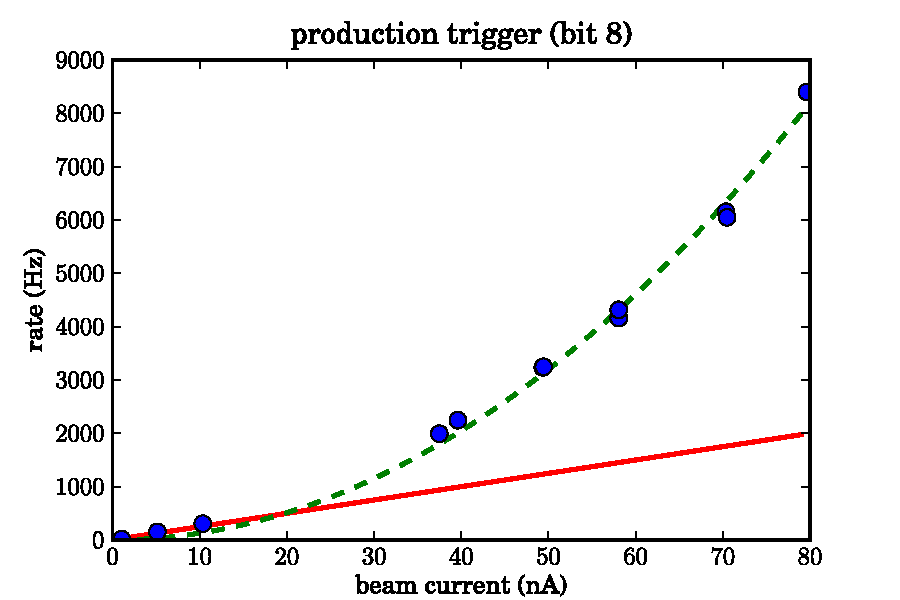
\includegraphics[width=0.6\columnwidth]{figures/calib/trig/trigger_study.eps}
\caption[Trigger Rate vs. Beam Current]{\label{fig:data.trig.eff}The production trigger rate (bit 8 in Tables~\ref{tab:data.trig.conf.1} and \ref{tab:data.trig.conf.2}) was measured for various beam currents shown by the blue dots. The rates below 10~nA are roughly linear and are extrapolated via the red solid line to show an estimate of the physical event rate. The actual trigger rate is fitted with a quadratic shown by the green dashed line. By this estimate, the accidental rate is shown to equal the physical event rate at approximately 40~nA. The \desg{g12} experiment was done at 60--65~nA.}
\end{center}\end{figure}

\FloatBarrier

\subsection{\label{sec:calib.tag}Tagger Timing Calibration}
The timing calibration of the tagger system was performed using the standard procedures. Overall, the quality of the calibration is excellent, showing an overall timing resolution of about $130~ps$, when the tagger time is compared with the RF time. The counter-by-counter alignment can be seen on Fig.~\ref{tagtpho}. The calibration was checked on a run by run basis (Fig.~\ref{tagRun}), and new constants were commissioned when major changes were noticed.

\begin{figure}[htpb]
\begin{center}
 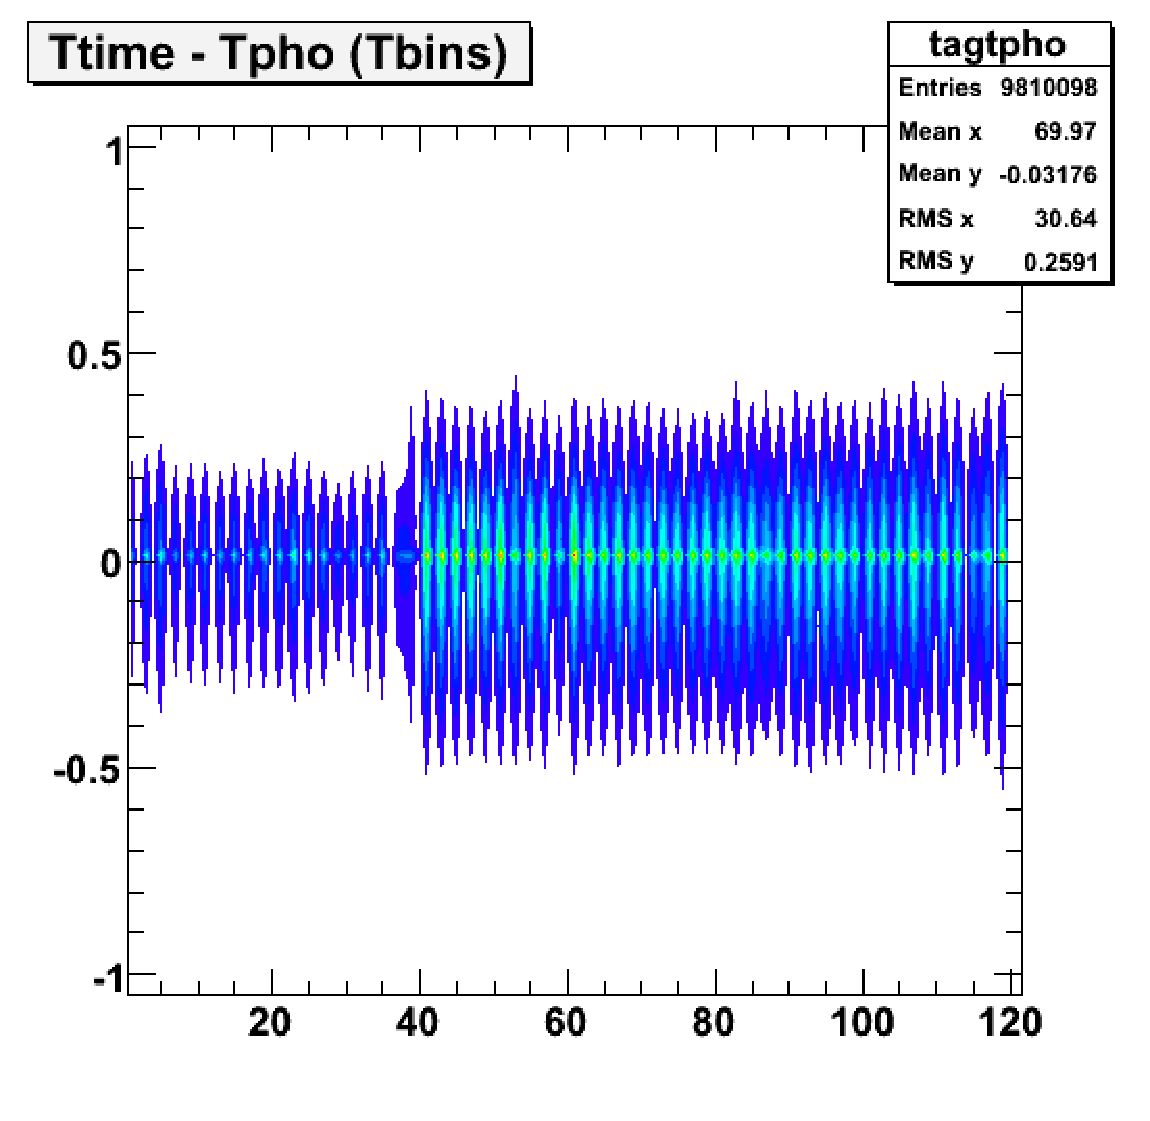
\includegraphics[width=0.45\textwidth]{figures/calib/tag/timing/tagtpho.eps}
  \caption{And example of the tagger timing calibration and the T-counter alignment, comparing  the difference between photon time determined from the tagger elements (T-counters, in this particular plot), and photon timing according to the RF. The relative intensity of the paddles shown are due to the trigger configuration, see Tables.~\ref{tab:data.trig.conf.2} and \ref{tab:data.trig.mor}.}
  \label{tagtpho}
  \end{center}
\end{figure}


\begin{figure}[htpb]
\begin{center}
 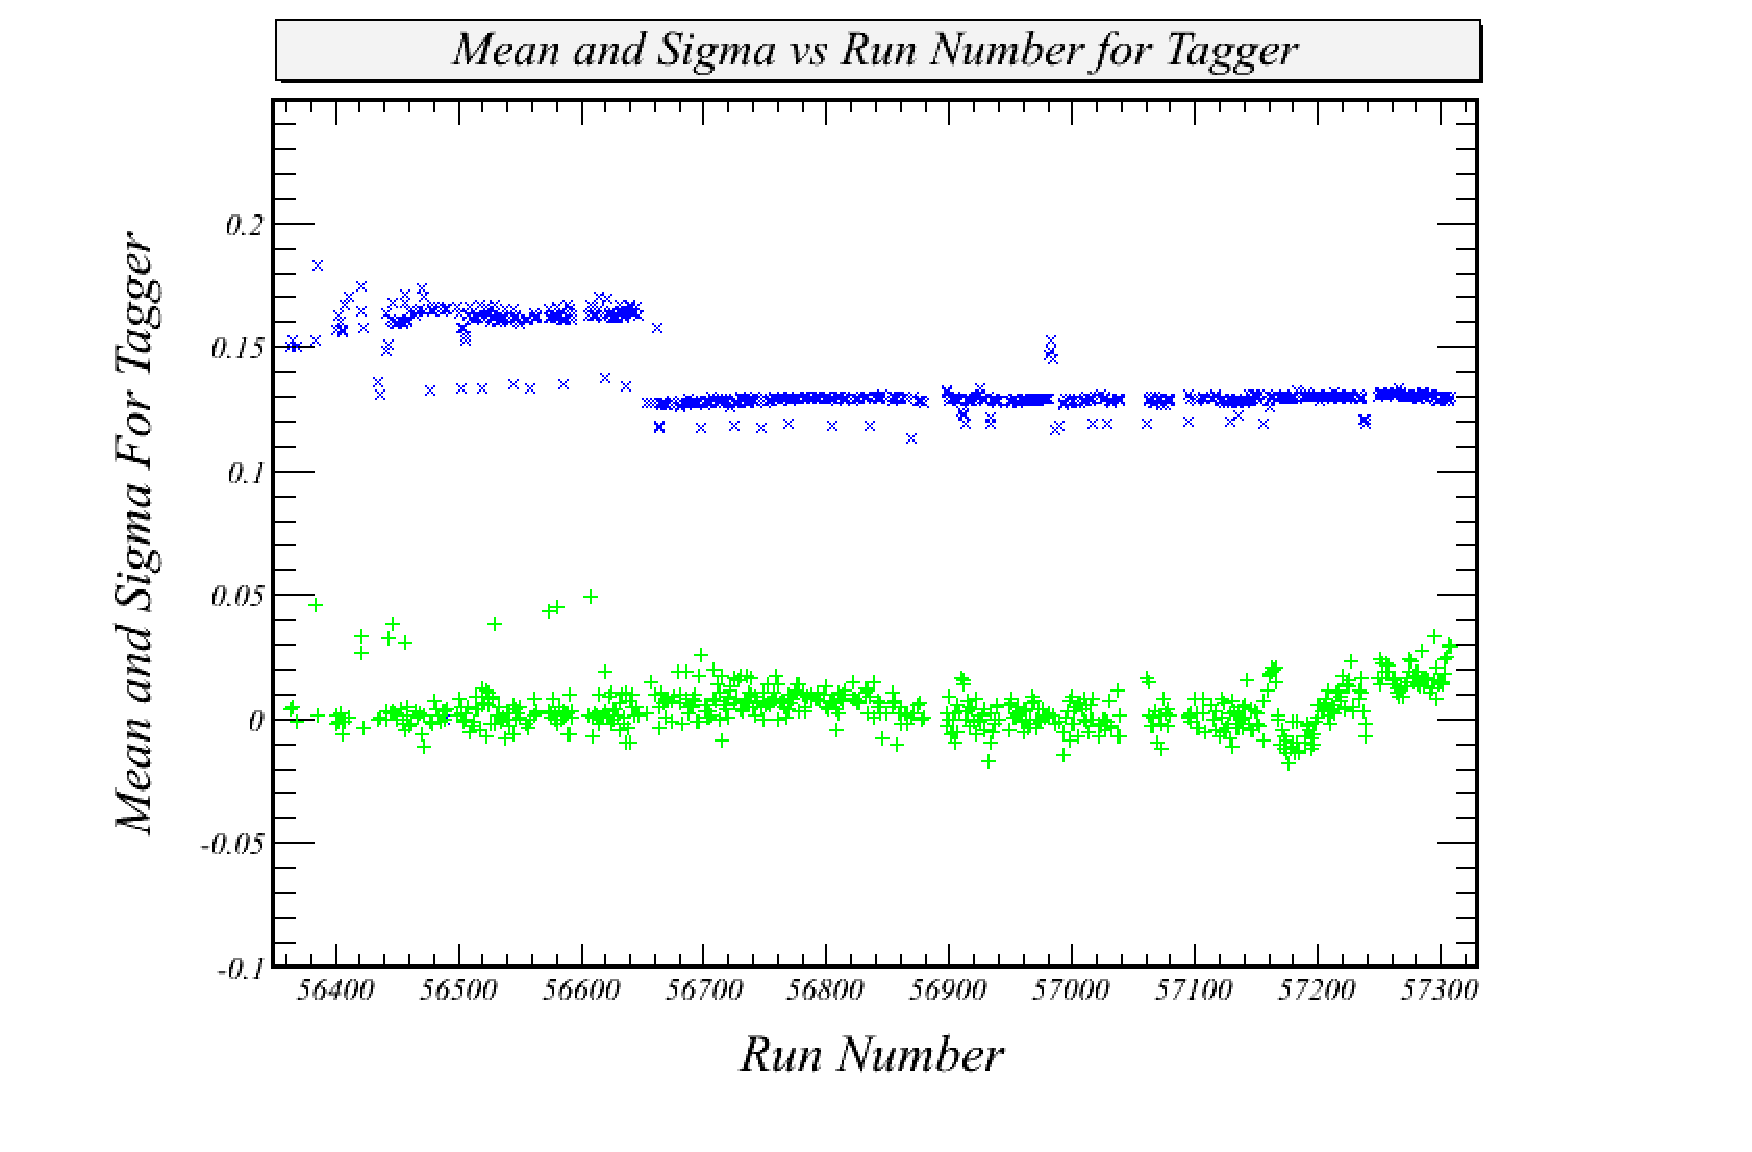
\includegraphics[width=0.45\textwidth]{figures/calib/tag/timing/tagRun.eps}
  \caption{The run-by-run behavior of the tagger timing calibration where the mean is in green and the sigma is in blue. Overall, the tagger timing resolution is about $130~ps$ for the production runs, and the mean behaves stably throughout the running period.}
  \label{tagRun}
  \end{center}
\end{figure}

\subsection{Target Density}\label{sec:analysis.target_density}

We need to know the target density to calculate the differential cross-section. The procedure for determining the density of $\ell$H$_2$ target in \abbr{CLAS} has already been established in ~\cite{clas.target.density}. In the \desg{g12} experiment, the target temperature and pressure was measured periodically during each run. Each run contained at least 3 measurements of the pressure and temperature. The formula for calculating the target density is;
% ~\cite{clas.target.density}
\begin{align}
\rho = a_1T^2 + a_2P +a_3 \label{eq:target_density} \ ,
\end{align}
where $T$ and $P$ represent the temperature and pressure respectively and $a_1$, $a_2$, $a_3$ are constants given in Tab.~\ref{tab:targetdensity} taken from ~\cite{mccarty}. Fig.~\ref{fig:target_density} shows the average target density, $\bar \rho$, for each run along with the $\sqrt{\sigma^2}$.
\begin{table}[h!]
\begin{minipage}{\textwidth}
\begin{center}
\begin{singlespacing}

\caption[Target Density Constants]{\label{tab:targetdensity}Constants used in target density measurements \vspace{0.75mm}}

\begin{tabular}{c|c}

%\hline \hline
%
%operation & \multicolumn{3}{c}{Generation} \\
%charge & I & II & III \\

\hline
Parameter & Value \\
\hline

$a_{1}$ & $-2.89 \cdot 10^{-5} \frac{g}{cm^3K^2}$  \\
$a_{2}$ & $1.0 \cdot 10^{-7} \frac{g}{cm^3mbar}$  \\
$a_{3}$ & $8.249 \cdot 10^{-2} \frac{g}{cm^3}$  \\
\hline \hline
\end{tabular}

\end{singlespacing}
\end{center}
\end{minipage}
\end{table}
\vspace{20pt}
The average density, for each run, was calculated as;
\begin{align}
\bar \rho_{run} = \frac{1}{N}\sum_i^N \rho_i \ ,
\end{align}
while the variance $\sigma^2$ is calculated, for each run, as;
\begin{align}
\sigma^2 = \frac{1}{N - 1}\sum_i^N (\rho_i - \bar \rho)^2 \ .
\end{align}
Once the target density was calculated for each run, the average target density for all \desg{g12} runs was calculated using;
\begin{align}
\bar \rho_{tot} = \frac{1}{N_{run}}\sum_i^{N_{run}} \bar \rho_{run} = 0.0711398 \pm 1.74 \cdot10^{-5}\ ,
\end{align}
while the variance $\sigma^2$ is calculated, for all \desg{g12} run, as;
\begin{align}
\sigma_{tot}^2 = \frac{1}{N_{run} -1}\sum_i^{N_{run}} (\bar \rho_{run} - \bar \rho_{tot})^2 = 0.00024 \ .
\end{align}
Since the uncertainty, $\sigma$, in the target density is lower than the uncertainty of the physical in the target materials, the target density uncertainty will not be a factor in the total systematic uncertainties. The target length has an inaccuracy of 0.2~cm. This gives a systematic of 0.5\%.

\begin{figure}[h!]\begin{center}
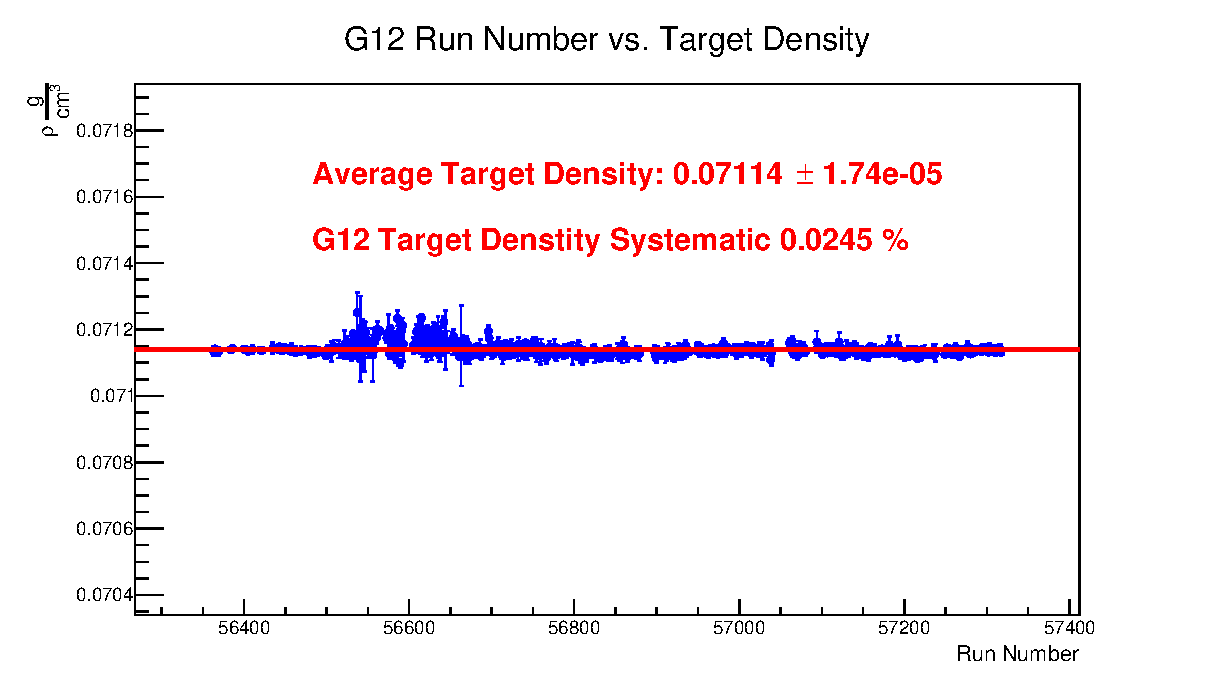
\includegraphics[width=0.9\textwidth]{figures/calib/targ/G12_Target_Density.eps}
\caption[Target density for \desg{g12}]{\label{fig:target_density}Target density for \desg{g12}. Image source:~\cite{clas.thesis.kunkel}}
\end{center}\end{figure}
\FloatBarrier

\subsection{\label{sec:calib.st}Start Counter Calibration and Resolution}

The start counter time-walk calibration took into account the varying geometry of the paddles. Fig.~\ref{fig:calib.st.adcuncor} shows the uncorrected timing difference for paddle 3 (of 24) as a function of \abbr{ADC} while Fig.~\ref{fig:calib.st.adccor} shows the corrected timing. This was done for each paddle and the resulting resolutions can be seen in Fig.~\ref{fig:calib.st.timepion} for pions, Fig.~\ref{fig:calib.st.timeproton} for protons, Fig.~\ref{fig:calib.st.timepion2d} for pions and all paddles, Fig.~\ref{fig:calib.st.timepion.ebeam} for pions a function of beam energy and Fig.~\ref{fig:calib.st.timepion.region} for pions as a function of geometry. The run-by-run resolution can be seen in Fig.~\ref{fig:calib.st.runbyrun}. This shows that the start counter was calibrated properly.

% ADC Uncorrected
\begin{figure}[htbp]\begin{center}
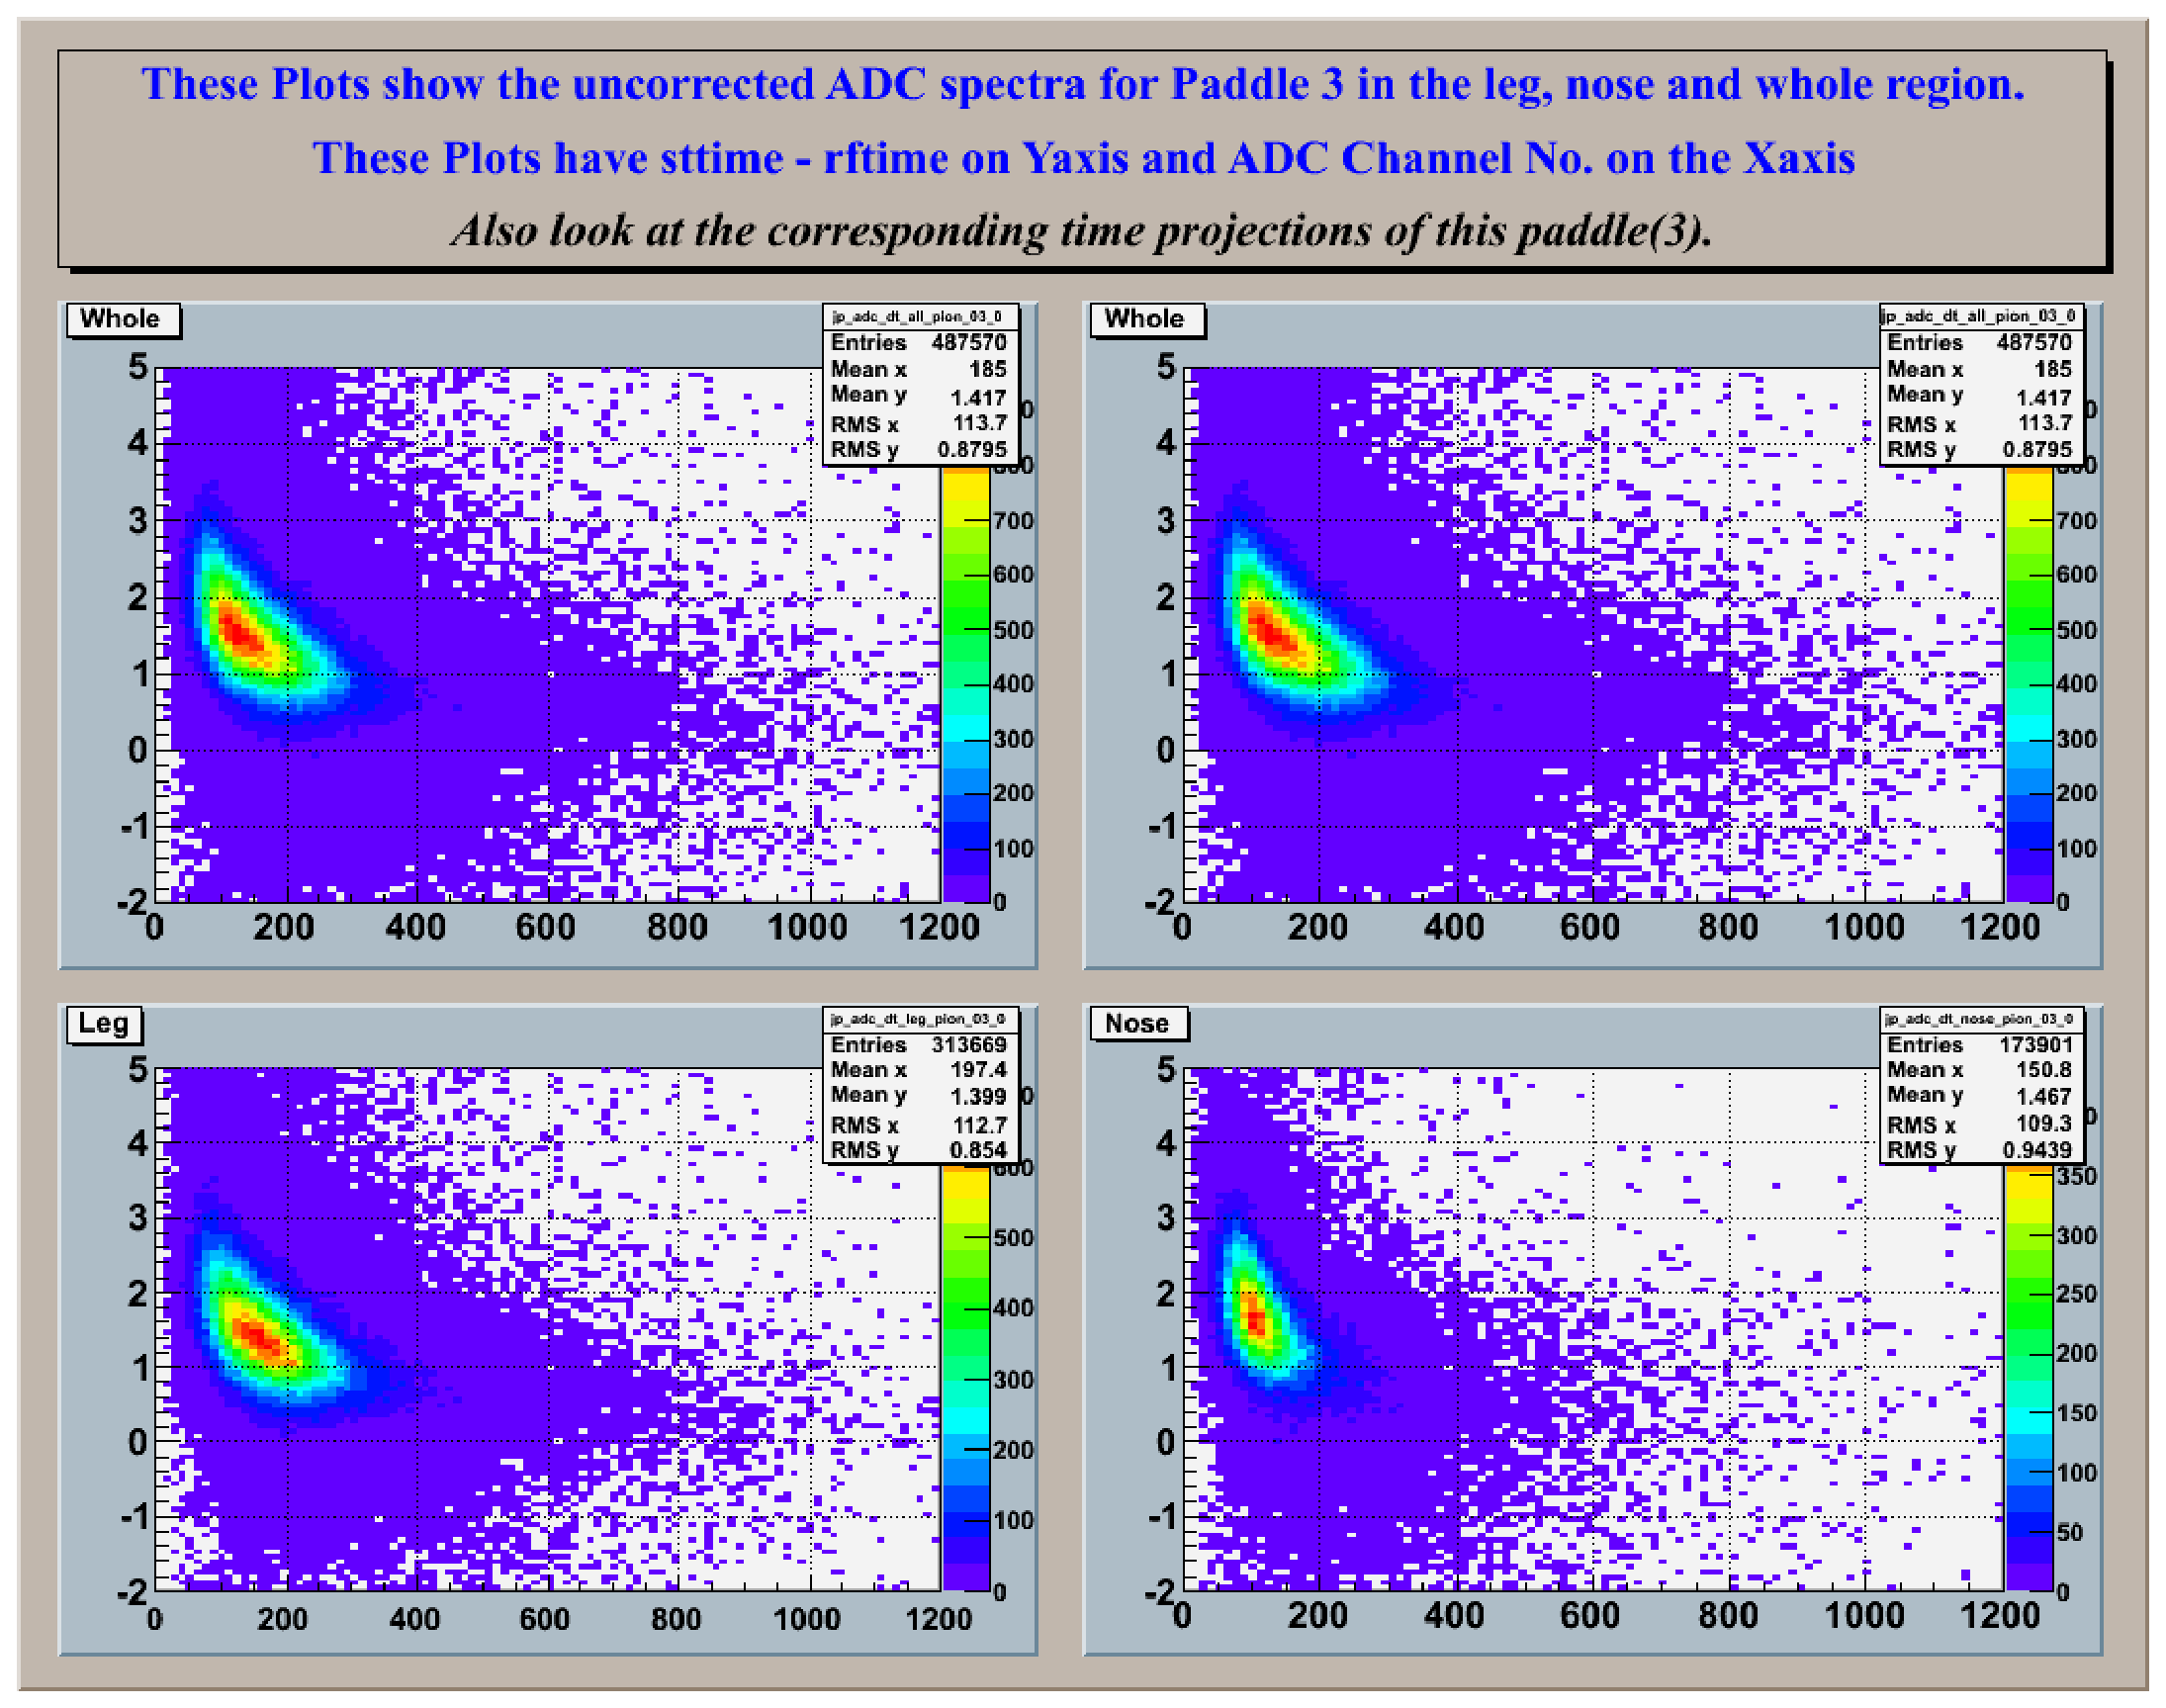
\includegraphics[width=0.65\columnwidth]{figures/calib/st/Uncorrected_adc.eps}
\caption[]{\label{fig:calib.st.adcuncor}ADC spectra for a paddle in the start counter. The top two plots are identical and show the all hits in the paddle. The bottom left plot shows hits in the ``leg'' of the counter and the bottom right shows hits in the ``nose.''}
\end{center}\end{figure}

% ADC Corrected
\begin{figure}[htbp]\begin{center}
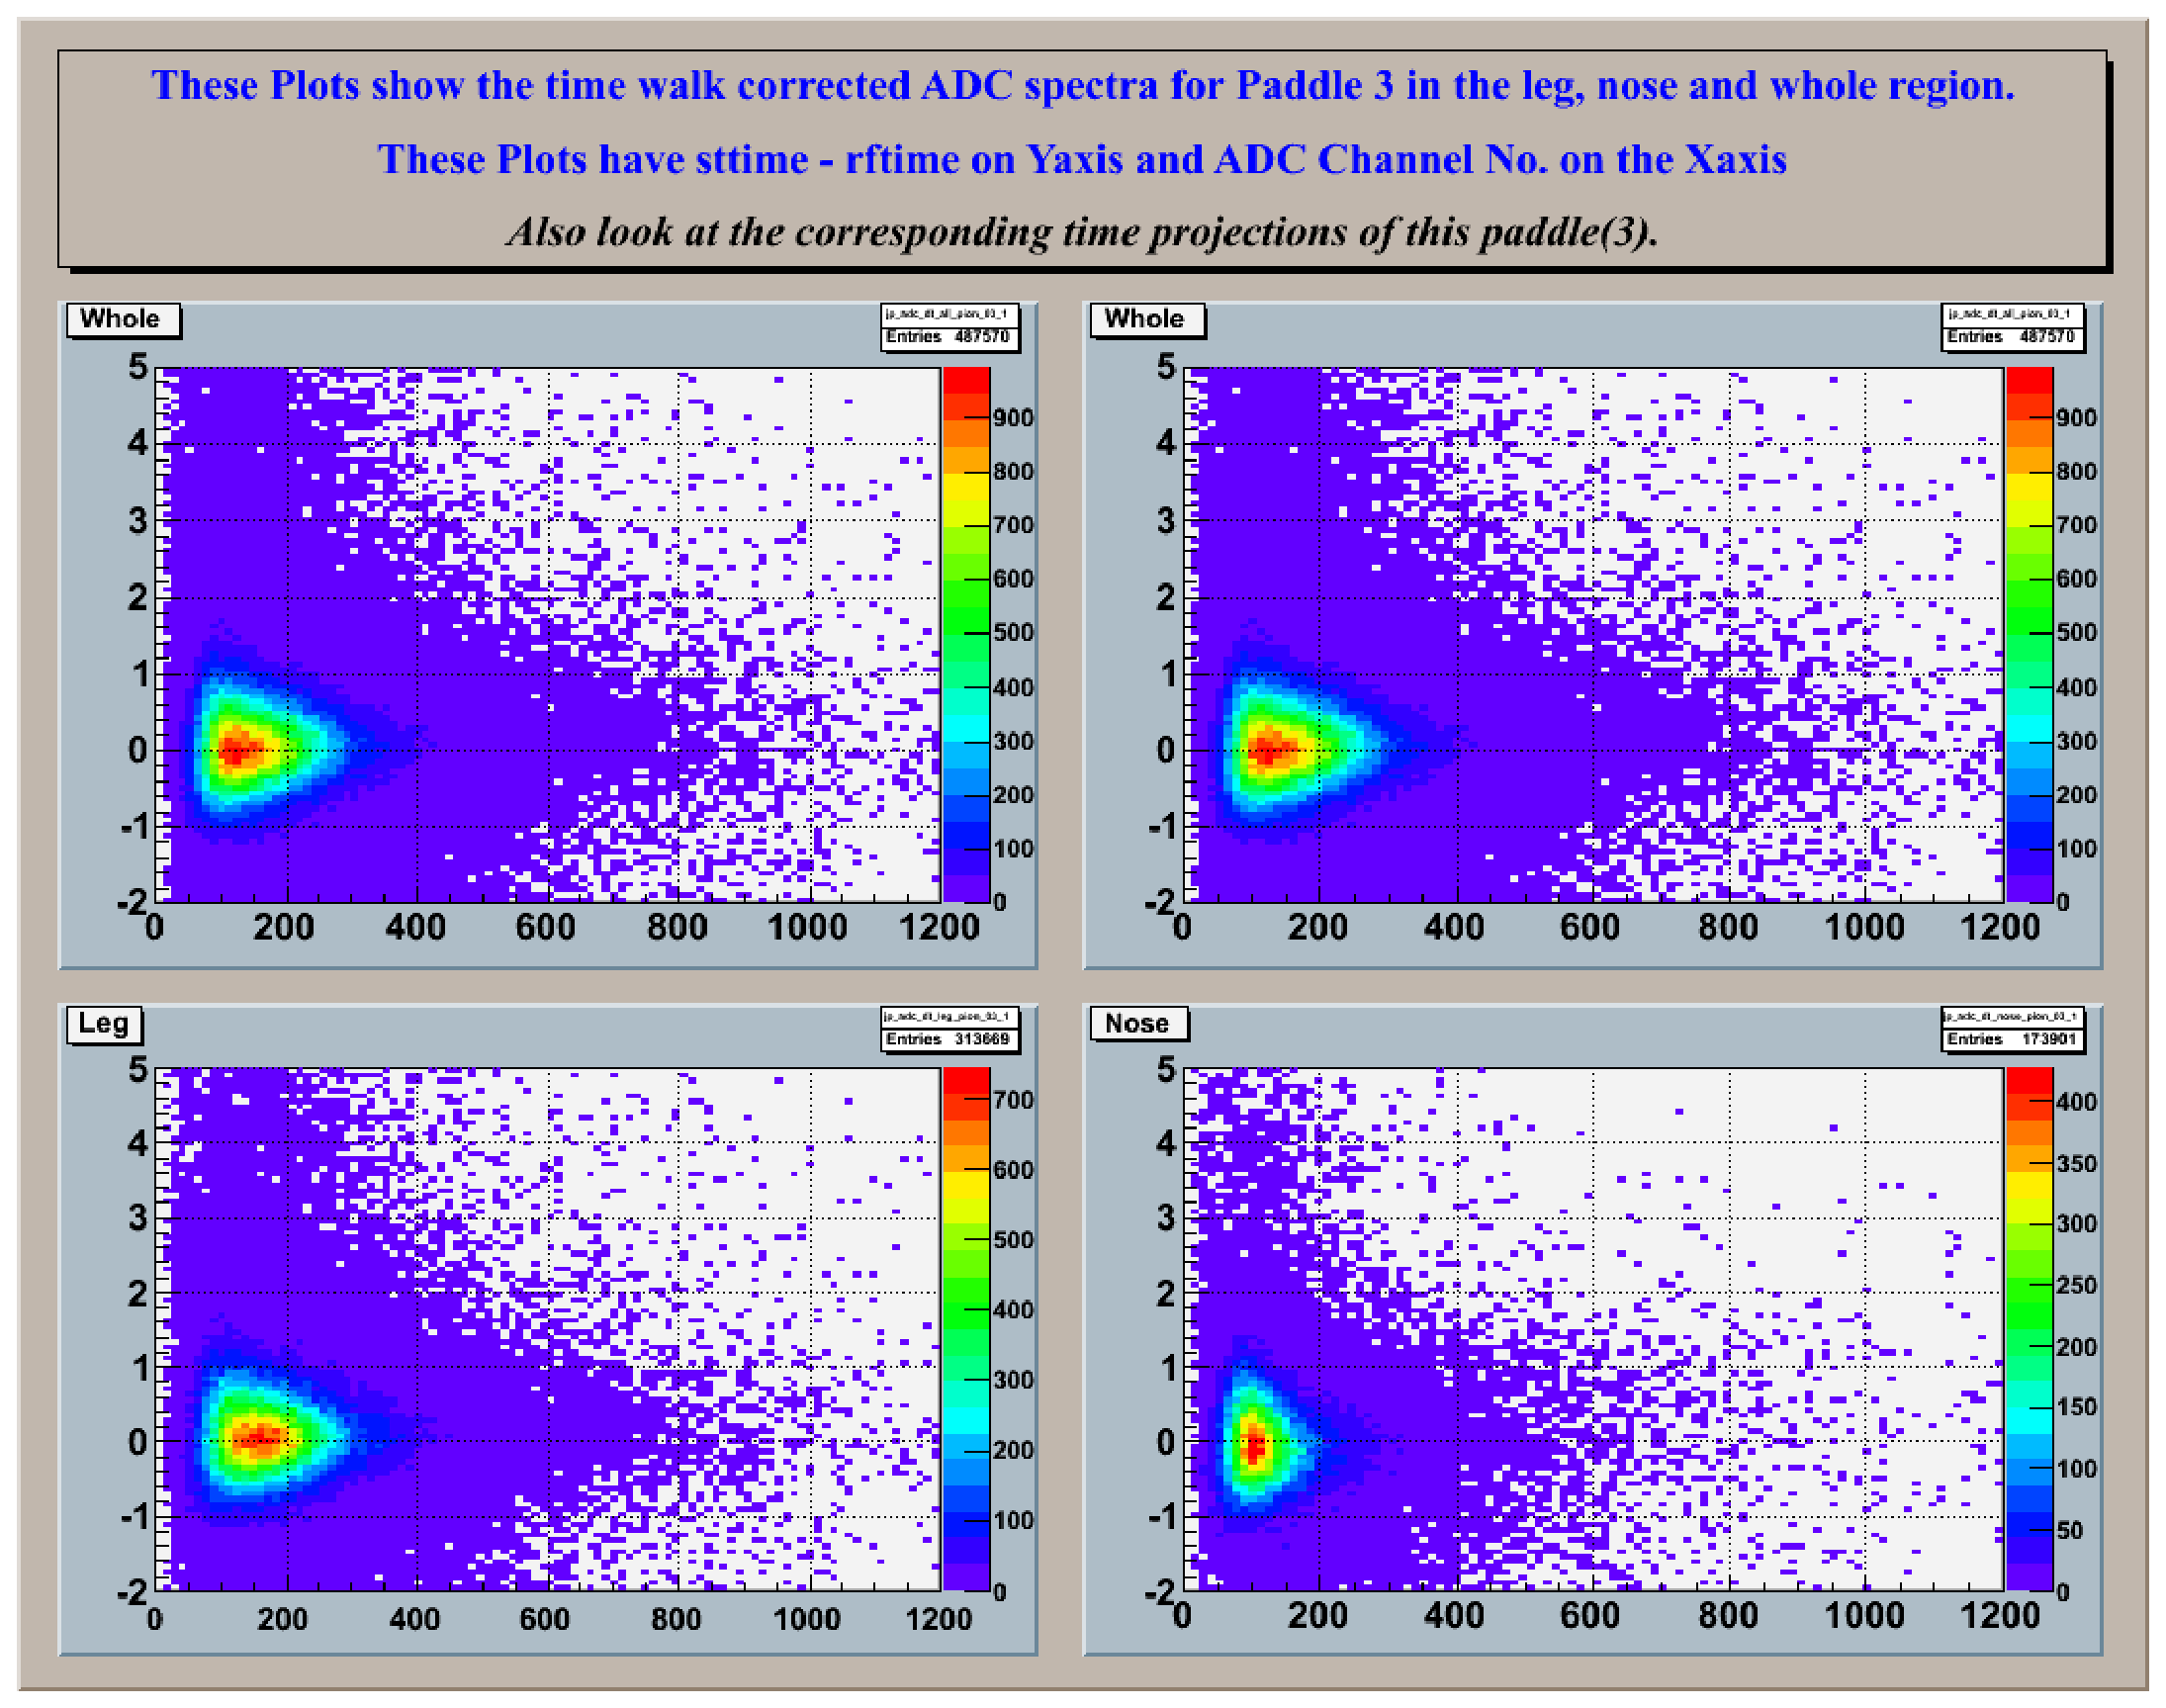
\includegraphics[width=0.65\columnwidth]{figures/calib/st/Corrected_adc.eps}
\caption[]{\label{fig:calib.st.adccor}See caption above and caption in Fig.~\ref{fig:calib.st.adcuncor}.}
\end{center}\end{figure}

\begin{figure}[htbp]\begin{center}
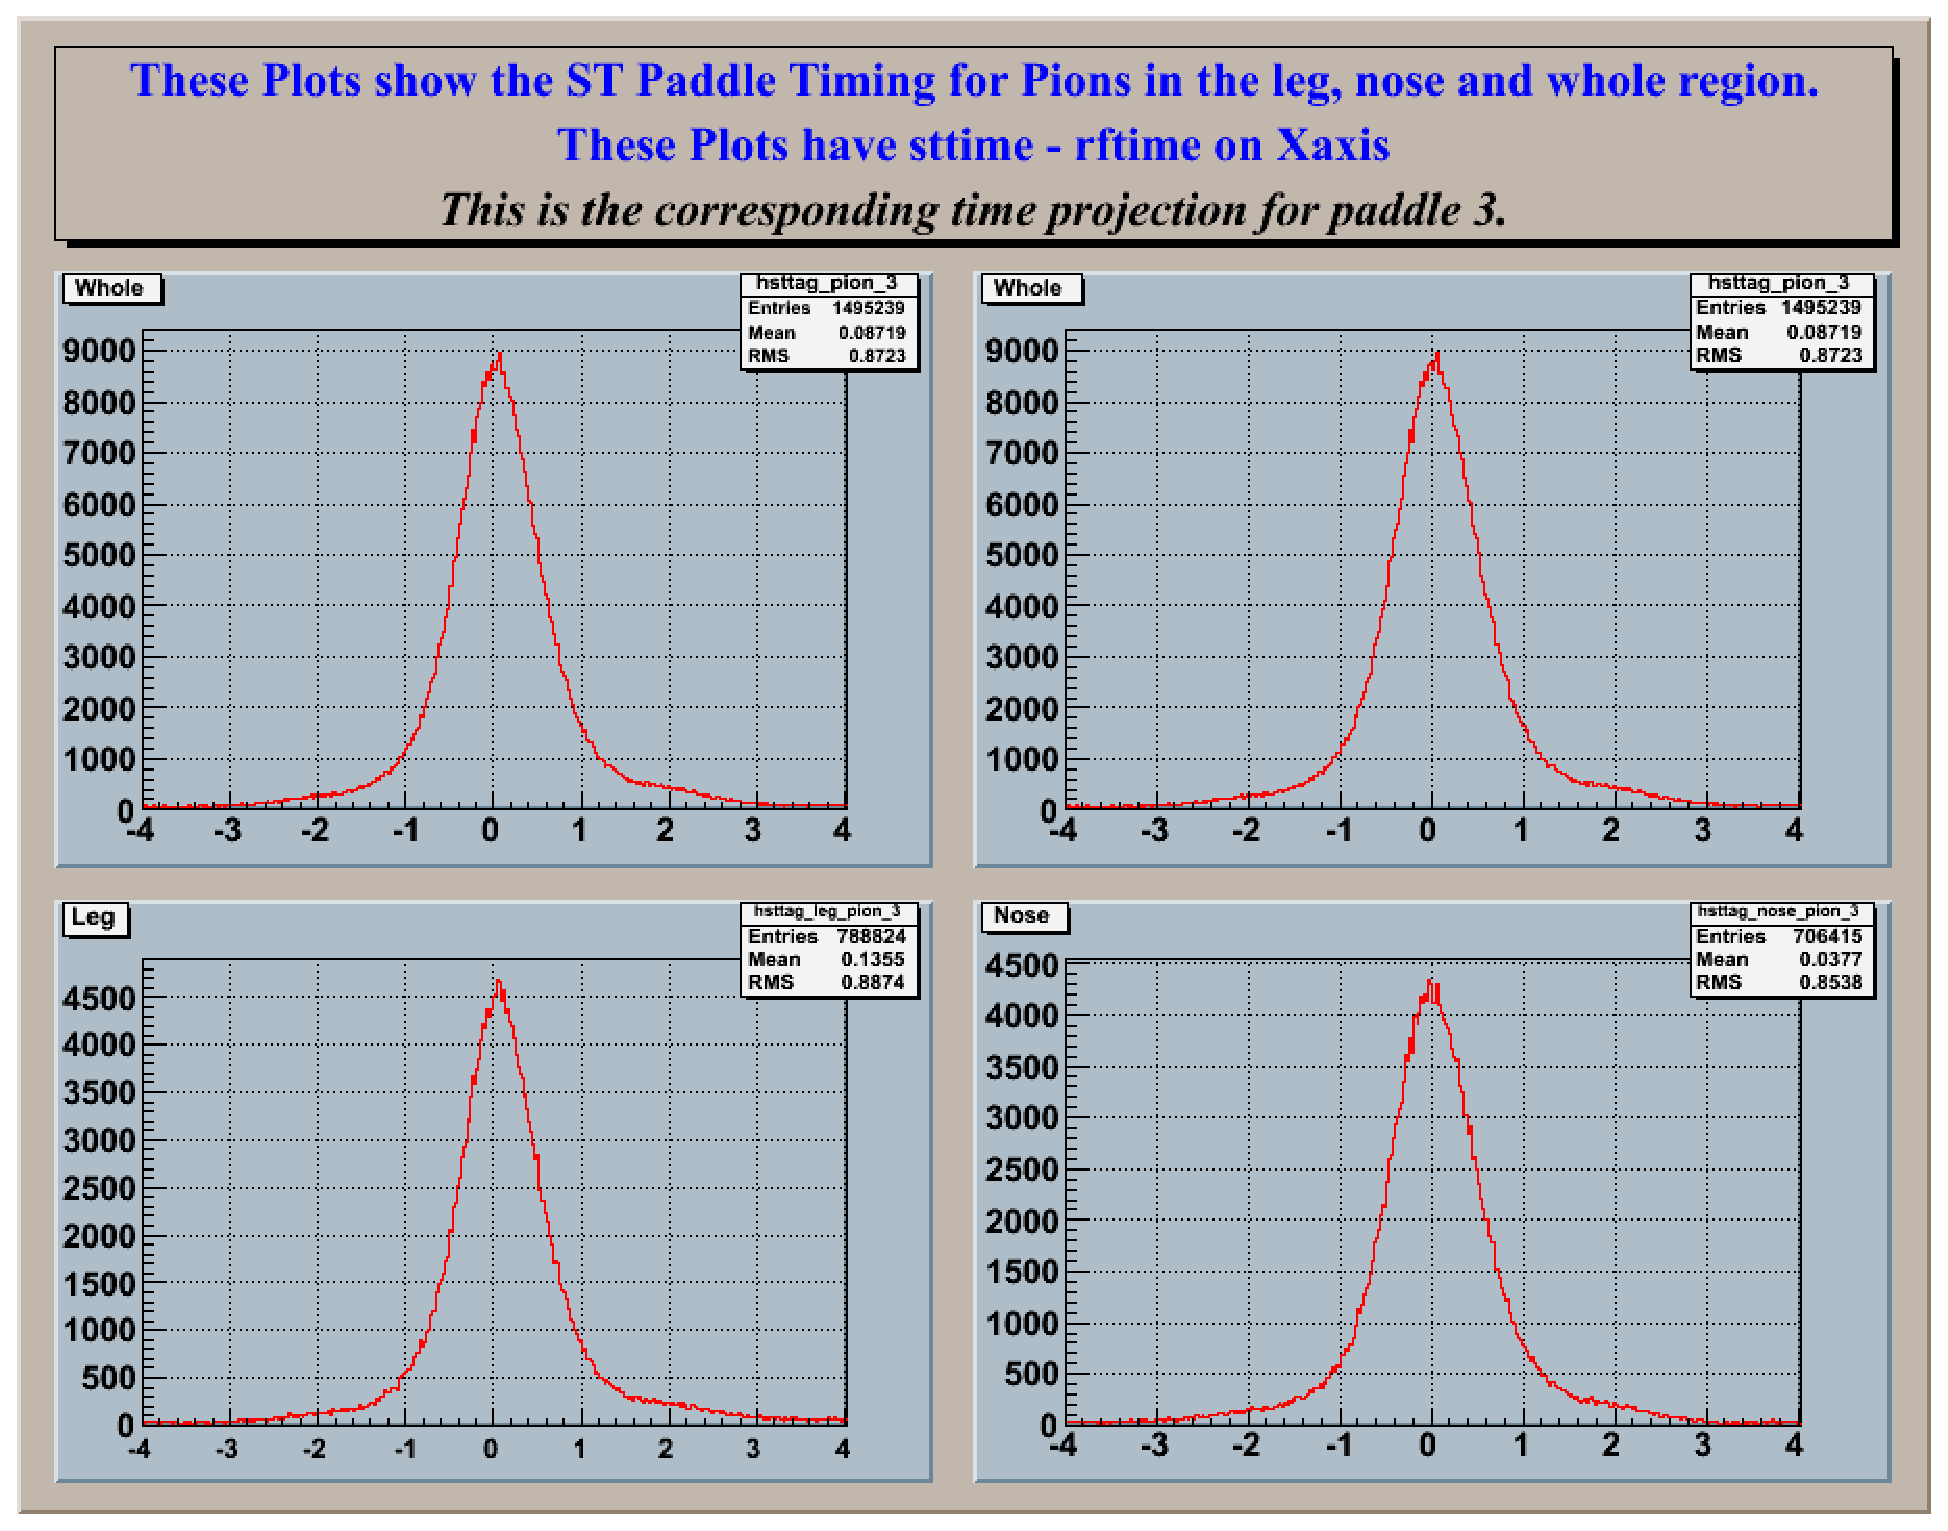
\includegraphics[width=0.65\columnwidth]{figures/calib/st/Hpad3_sttag_pion.eps}
\caption[]{\label{fig:calib.st.timepion}Difference of timing in a paddle of the start counter and the RF time for pions. The top two plots are identical and show the all hits in the paddle. The bottom left plot shows hits in the ``leg'' of the counter and the bottom right shows hits in the ``nose.''}
\end{center}\end{figure}

\begin{figure}[htbp]\begin{center}
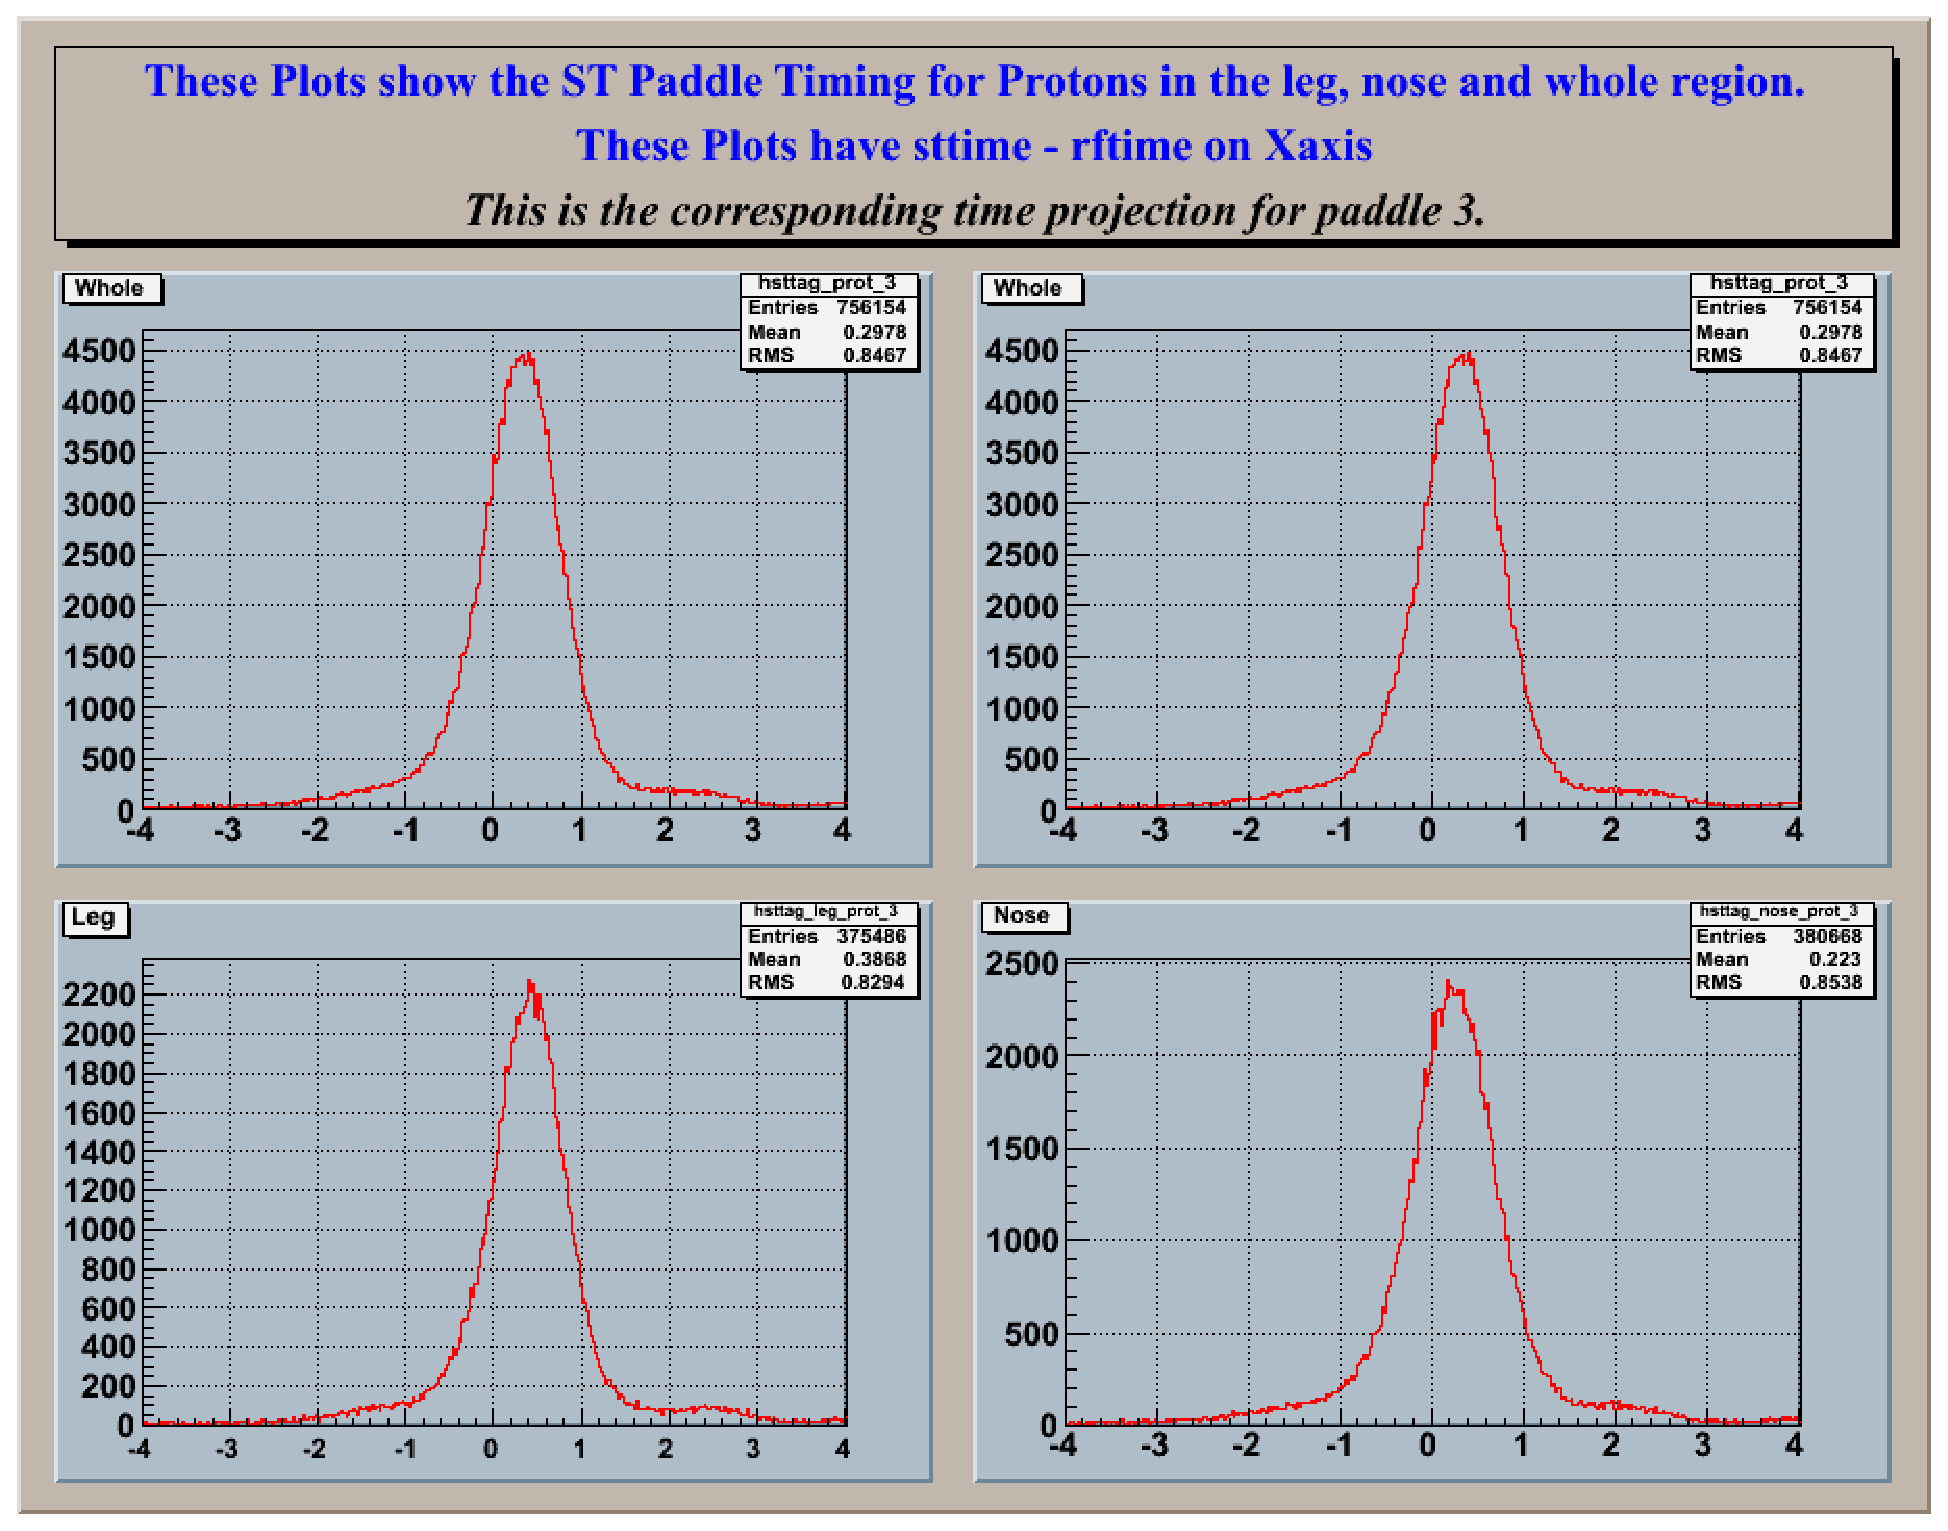
\includegraphics[width=0.65\columnwidth]{figures/calib/st/Hpad3_sttag_prot.eps}
\caption[]{\label{fig:calib.st.timeproton}Same as Fig.~\ref{fig:calib.st.timepion} for protons.}
\end{center}\end{figure}

\begin{figure}[htbp]\begin{center}
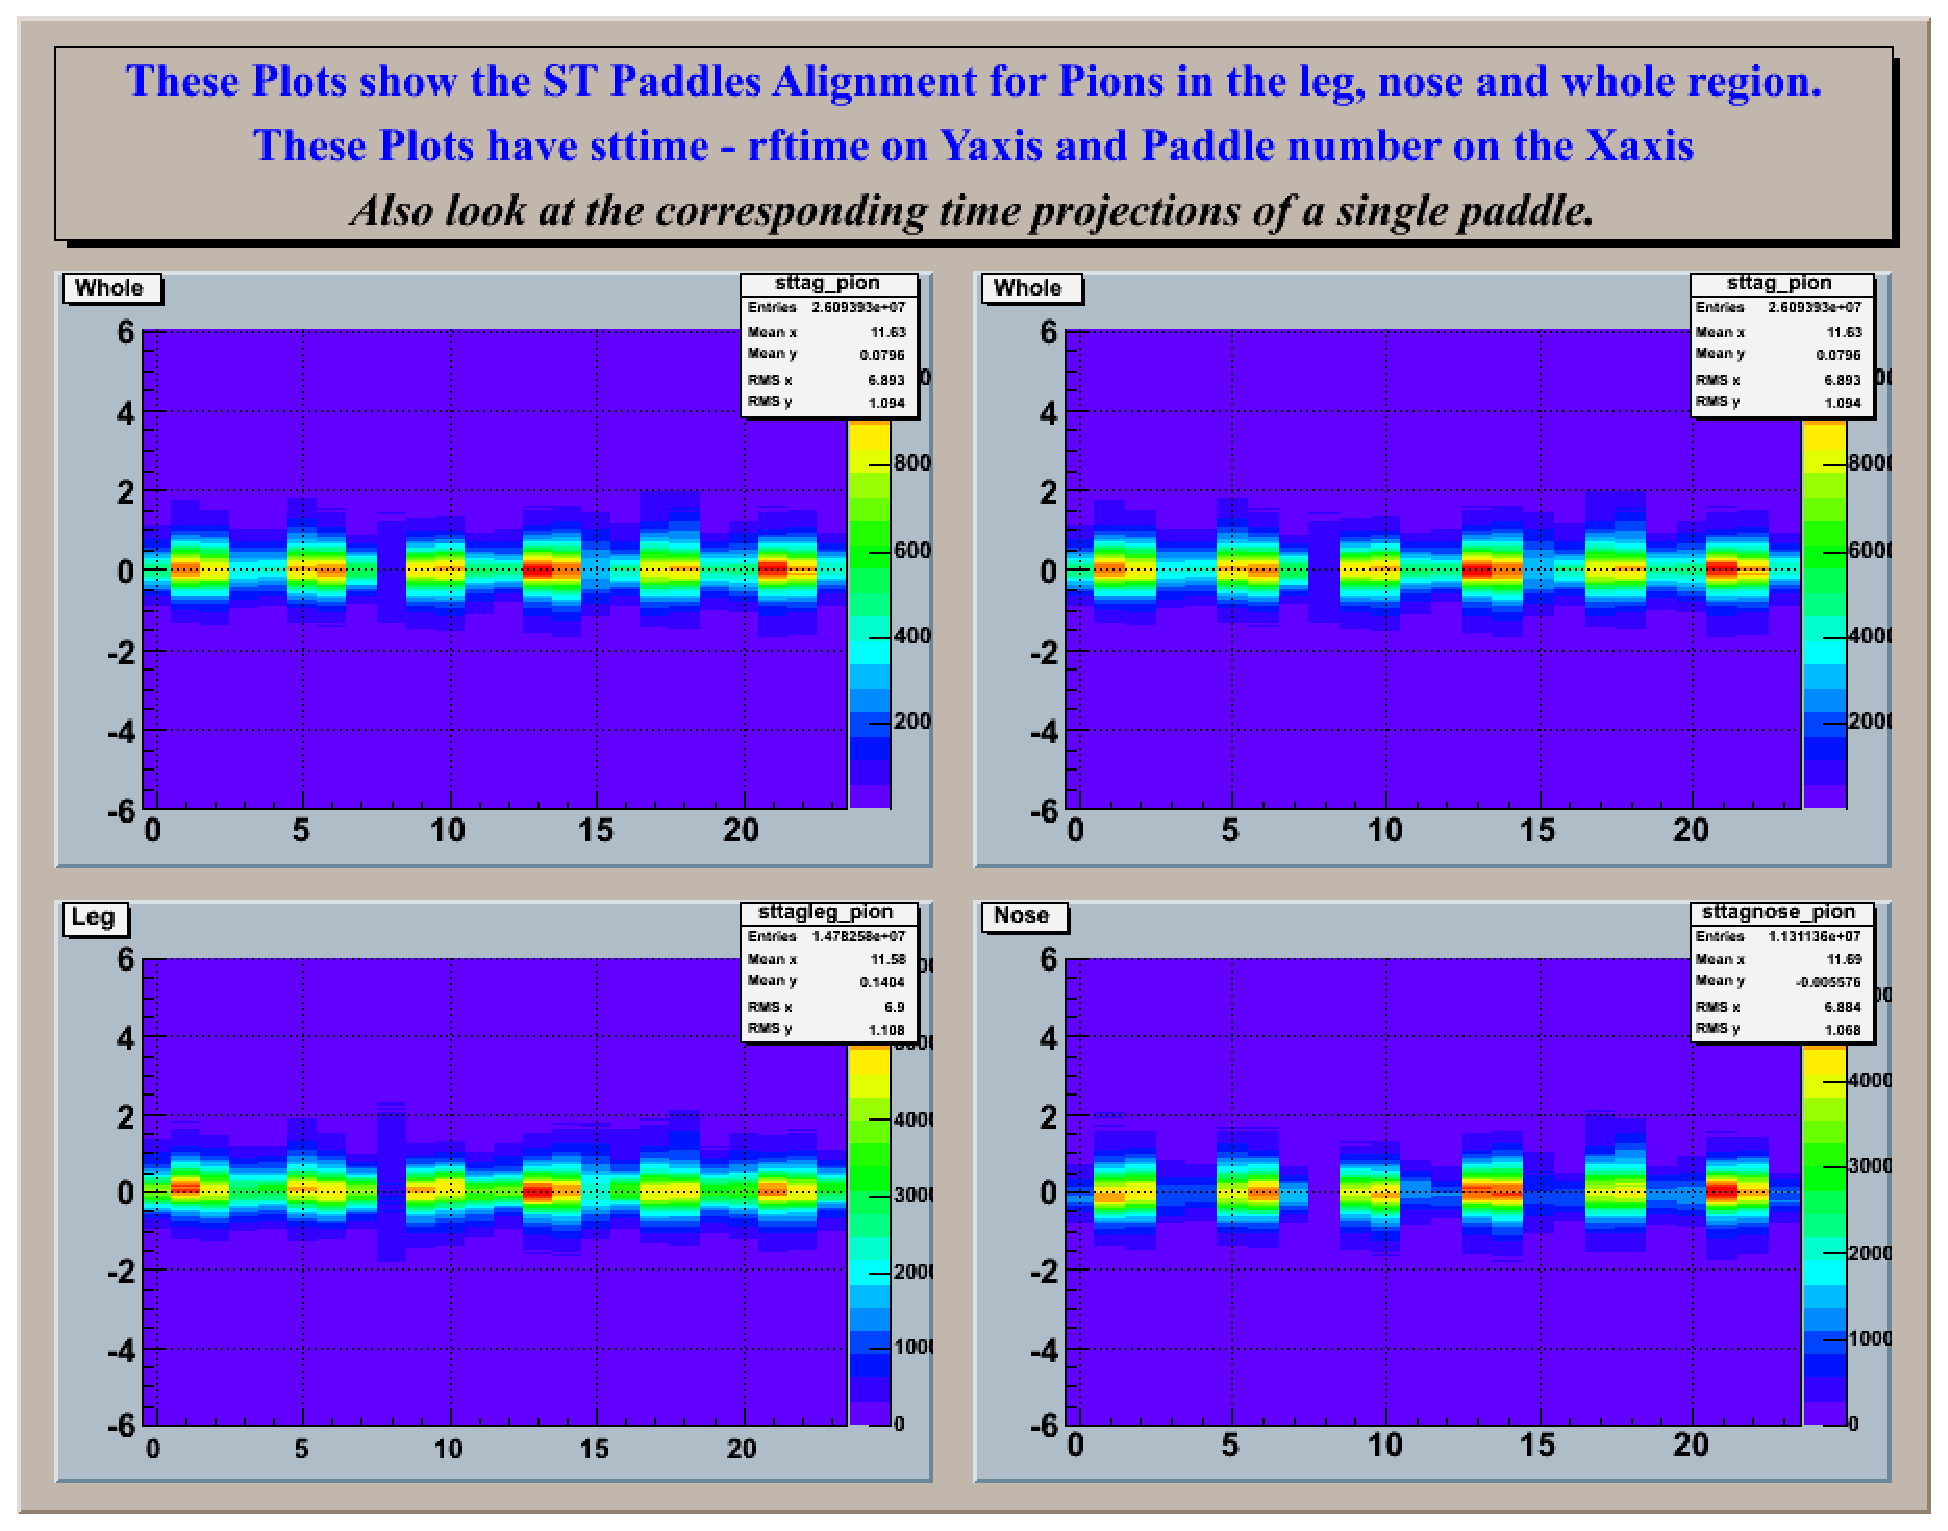
\includegraphics[width=0.6\columnwidth]{figures/calib/st/Hsttag_pion.eps}
\caption[]{\label{fig:calib.st.timepion2d}See caption above.}
\end{center}\end{figure}

\begin{figure}[htbp]\begin{center}
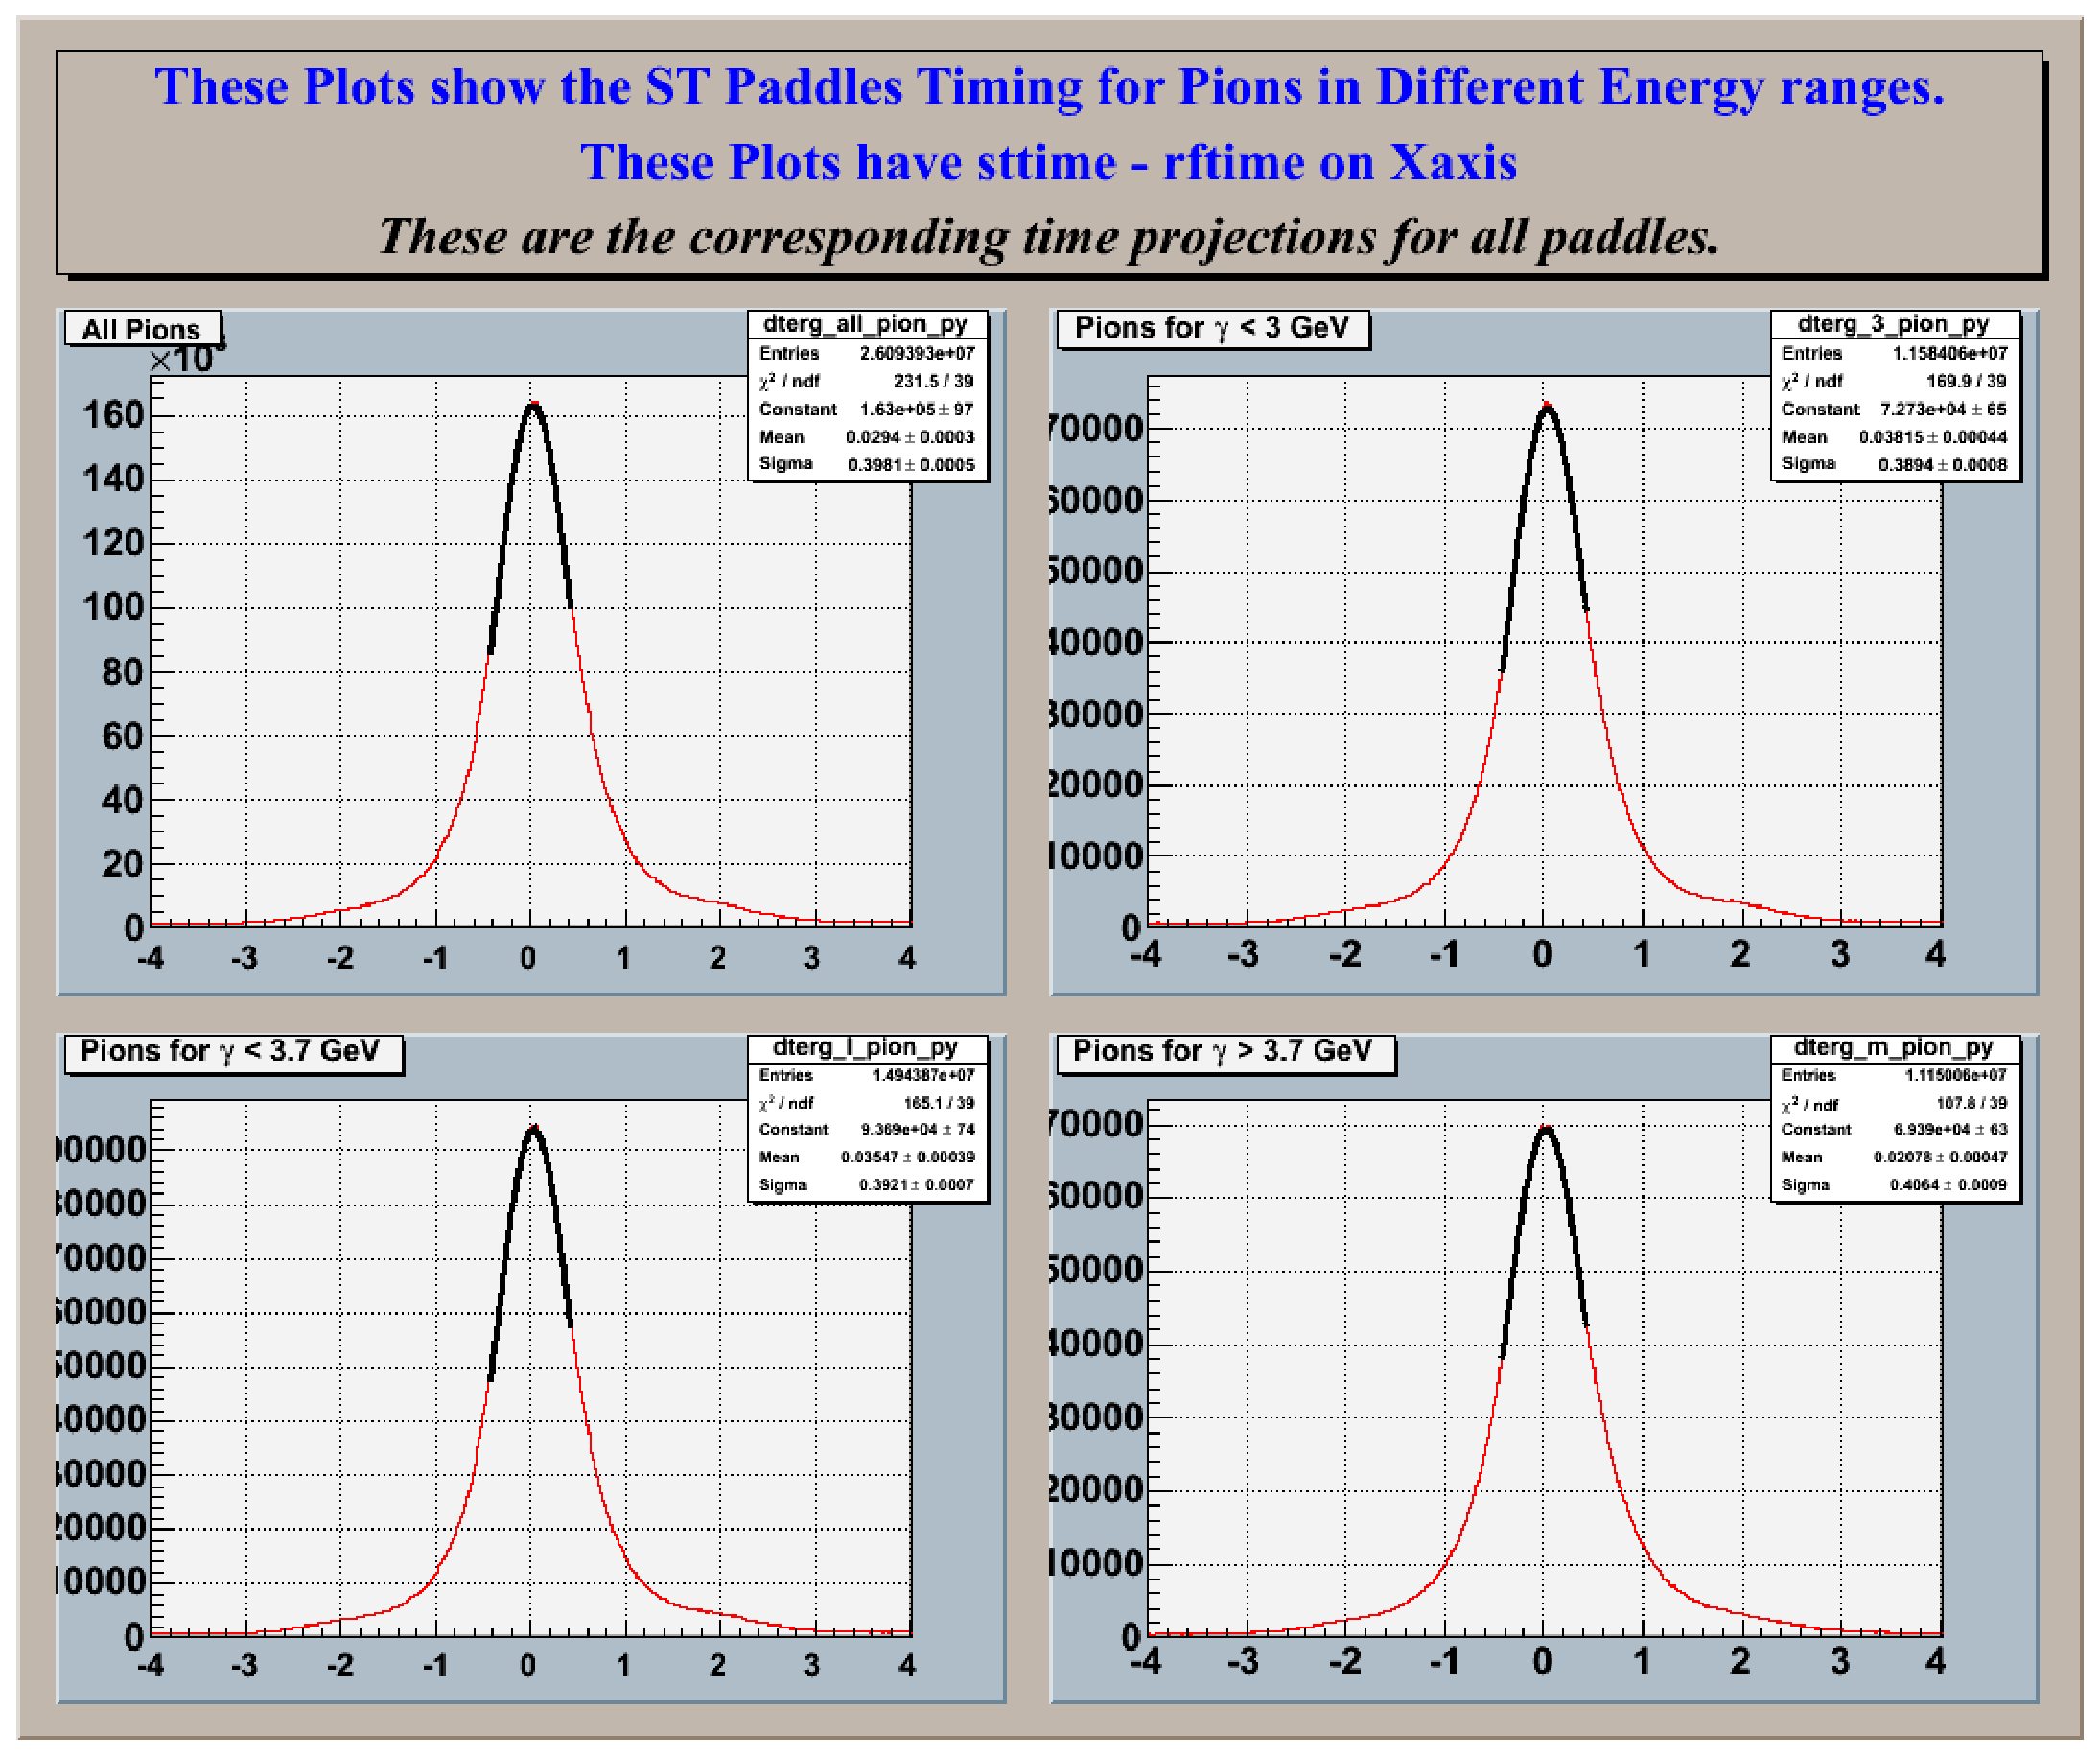
\includegraphics[width=0.6\columnwidth]{figures/calib/st/Sterg_pion.eps}
\caption[]{\label{fig:calib.st.timepion.ebeam}See caption above.}
\end{center}\end{figure}

\begin{figure}[htbp]\begin{center}
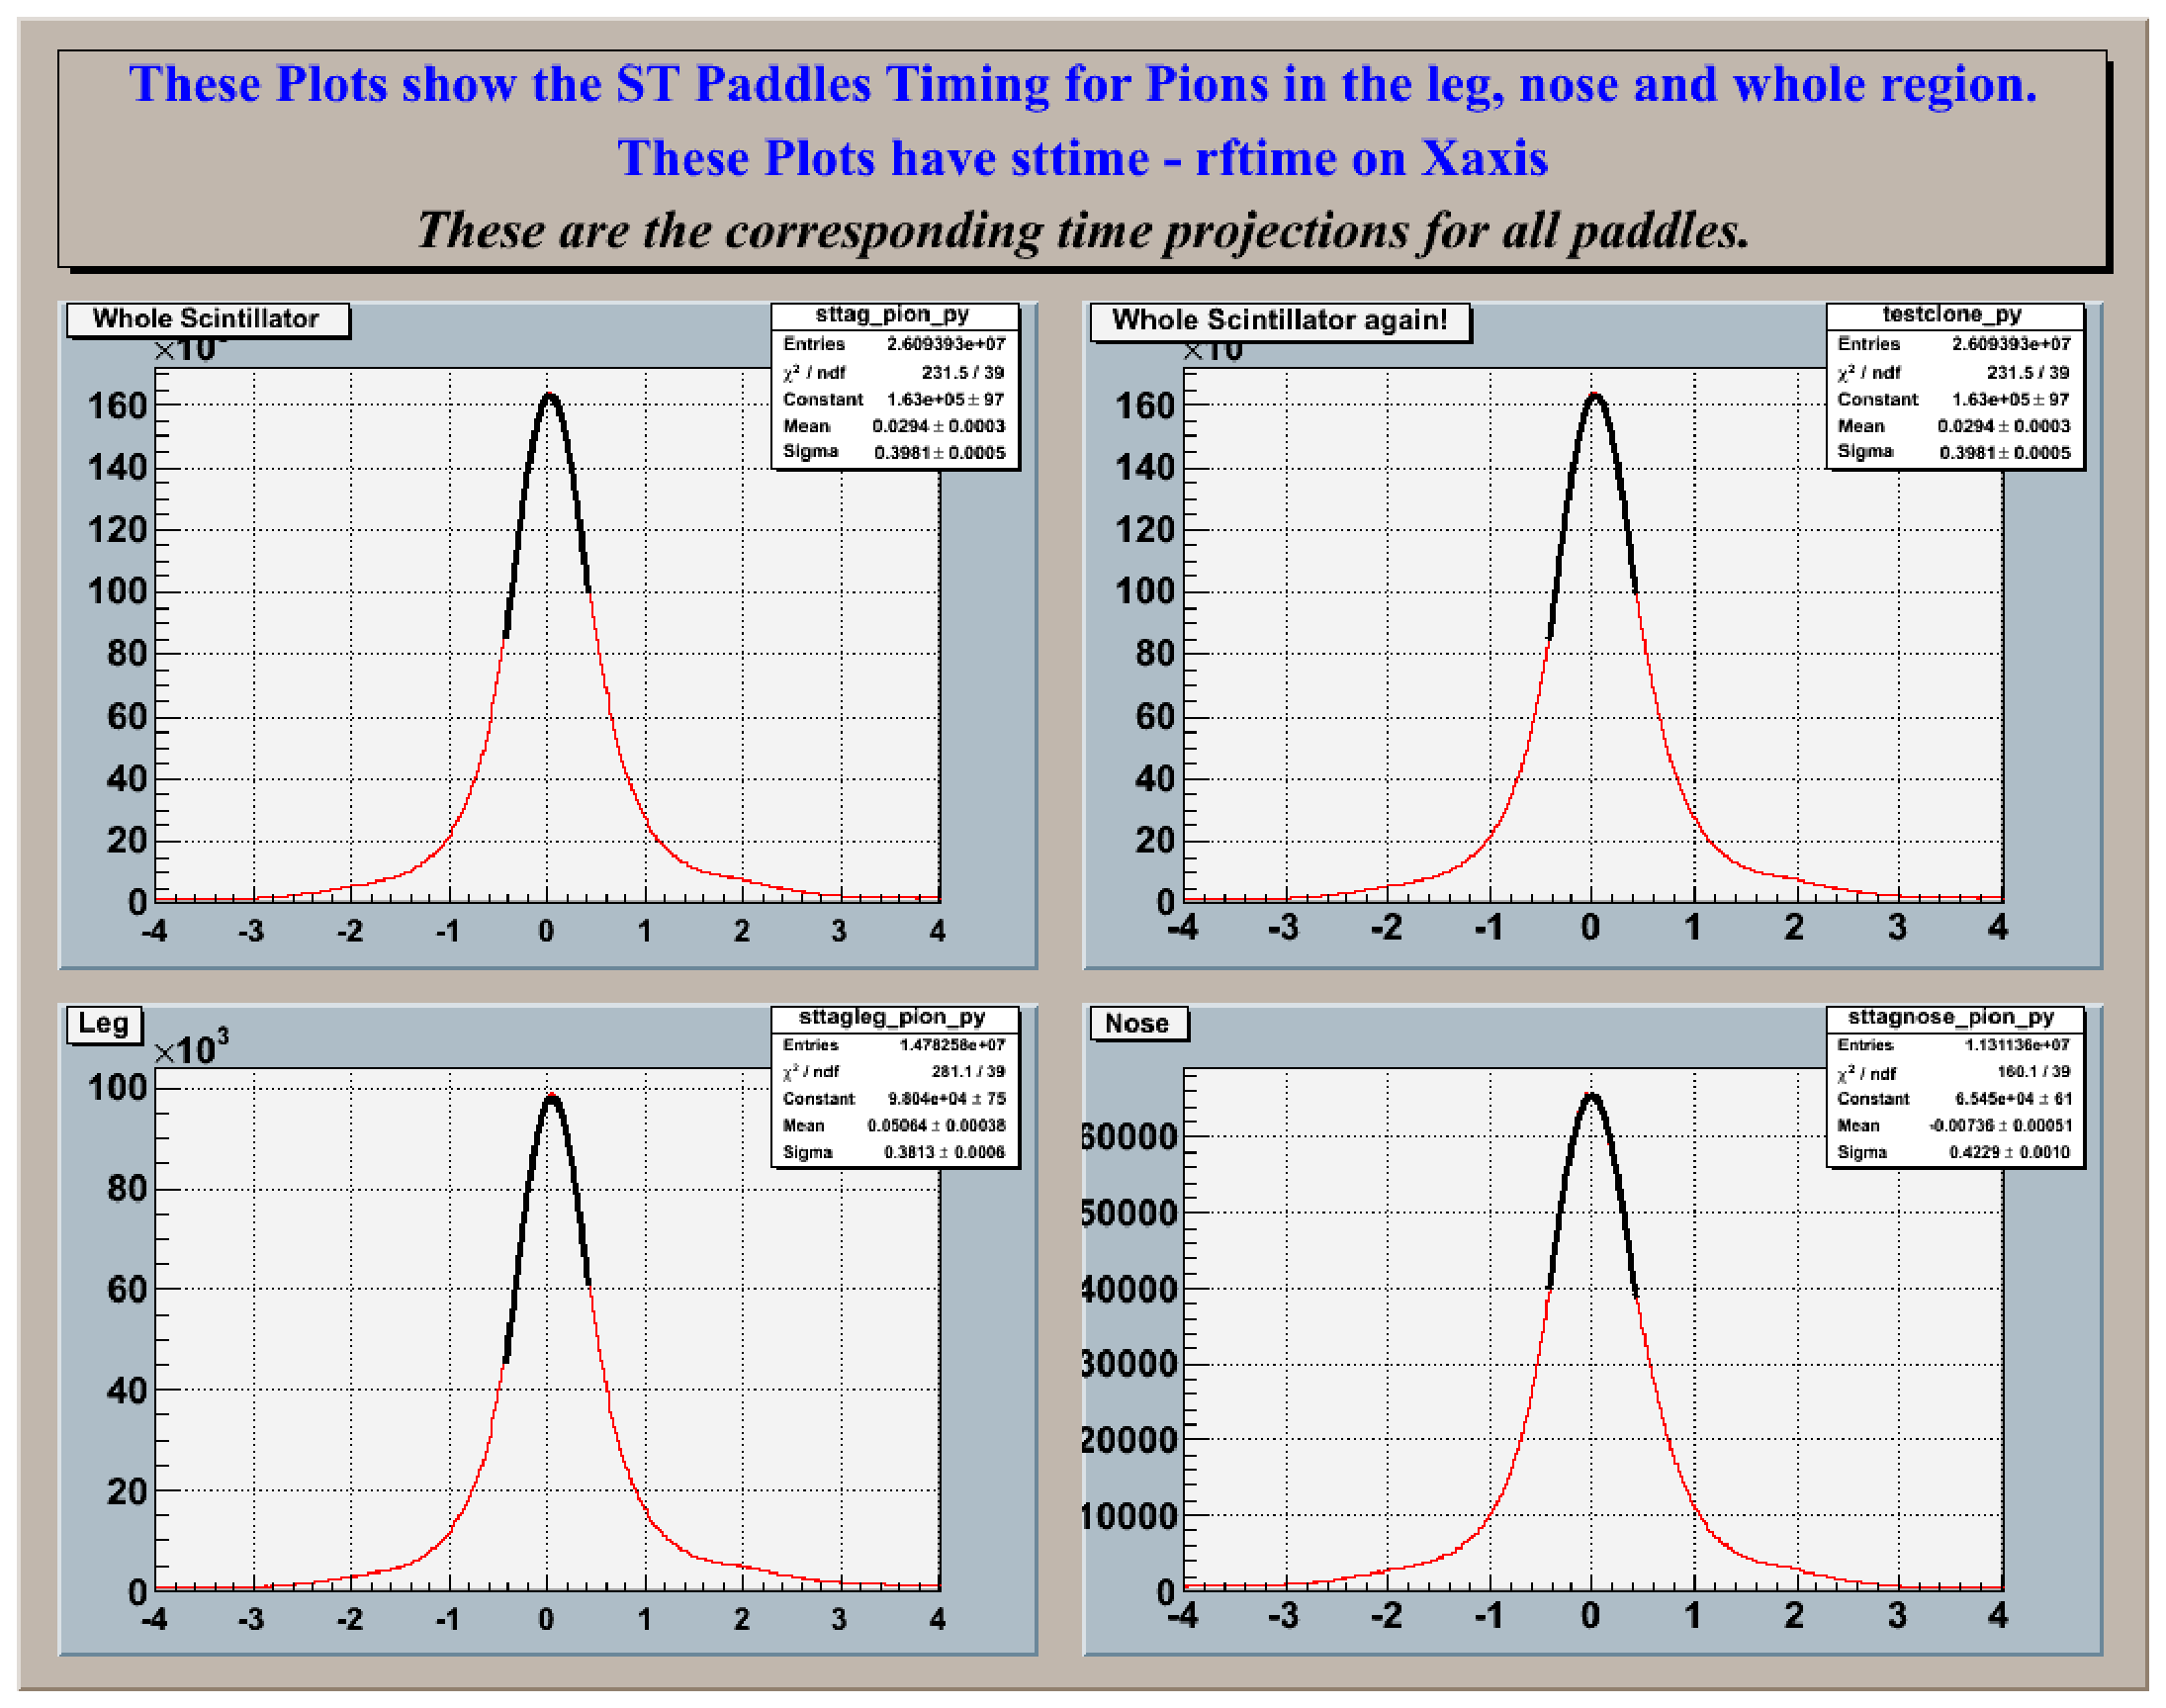
\includegraphics[width=0.6\columnwidth]{figures/calib/st/Timing_pad_3.eps}
\caption[]{\label{fig:calib.st.timepion.region}See caption above.}
\end{center}\end{figure}

\begin{figure}[htbp]\begin{center}
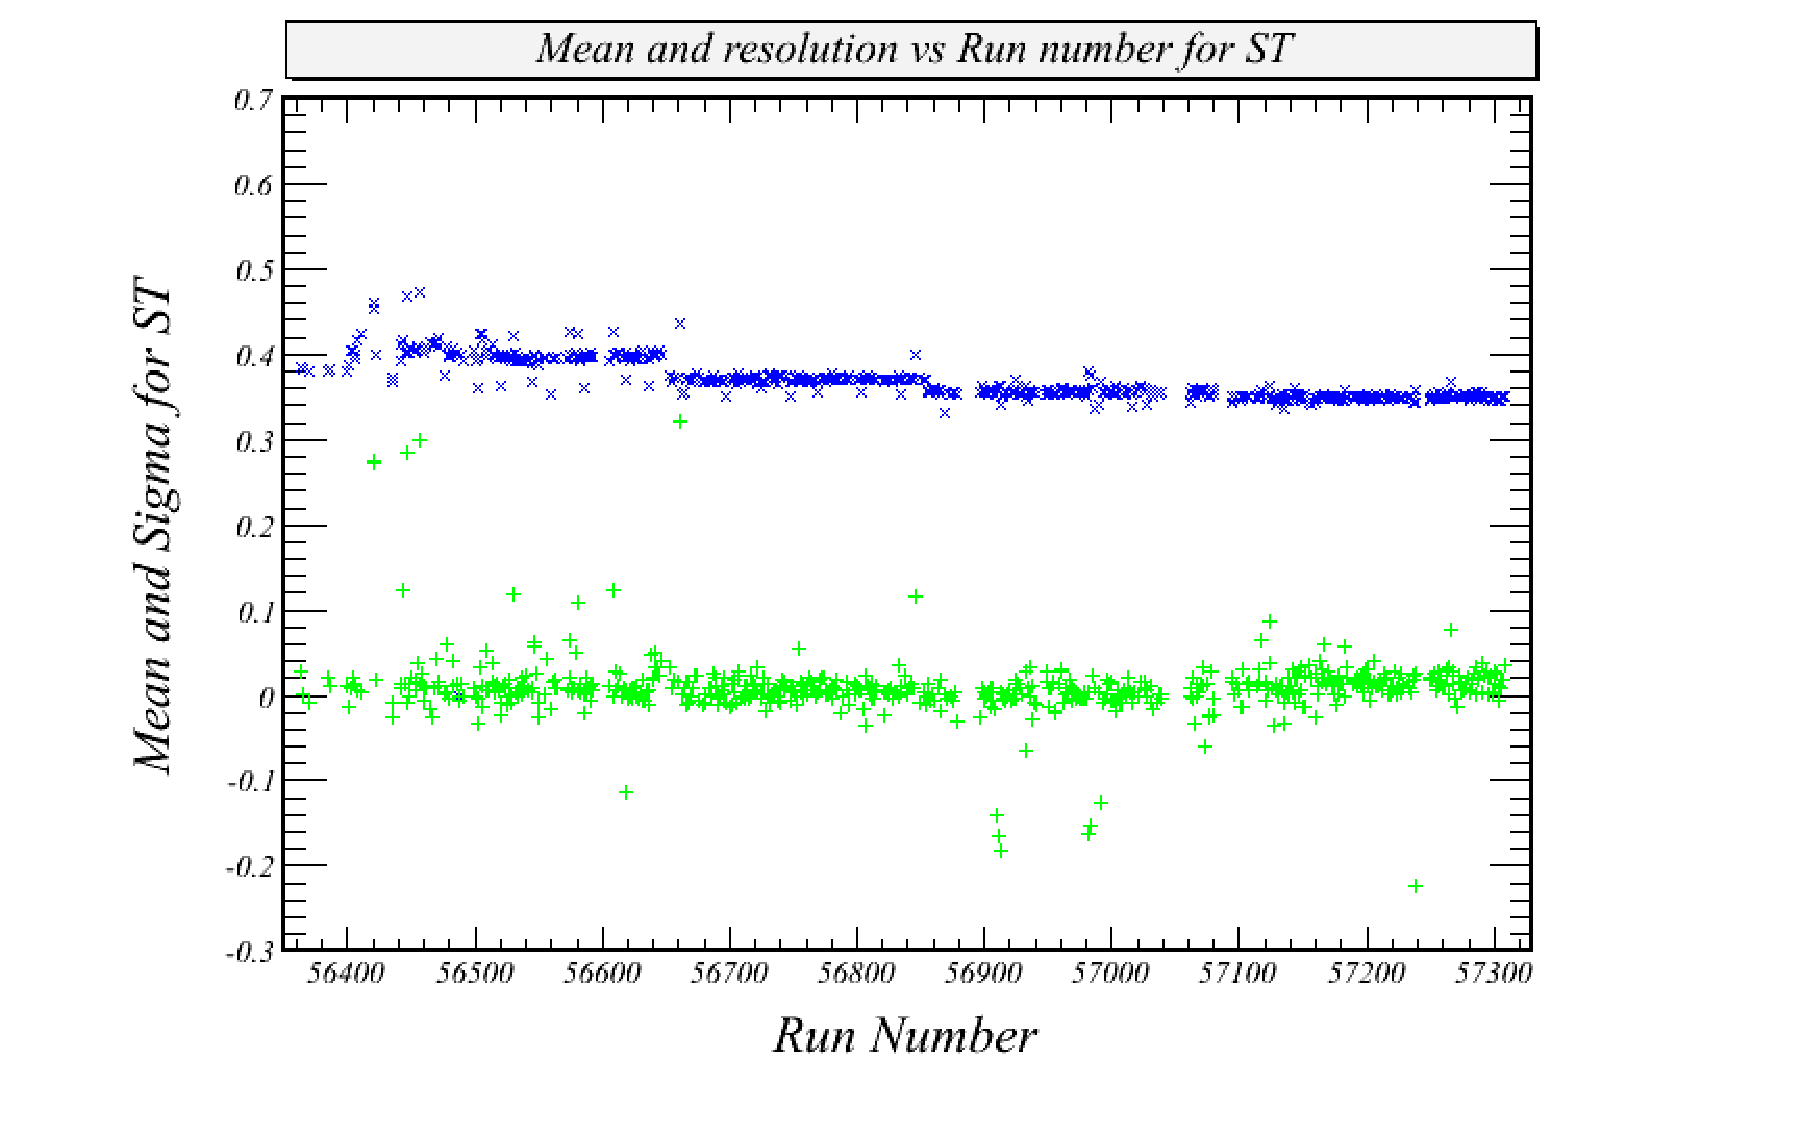
\includegraphics[width=0.65\columnwidth]{figures/calib/st/STmeanandres_v5.eps}
\caption[]{\label{fig:calib.st.runbyrun}Calibrated difference in time between the start counter and RF as a function of run. The mean (green) and 1σ resolution (blue) are shown.}
\end{center}\end{figure}

\FloatBarrier

%%%%%% add ref to 13,14


As a check on the timing resolution of the start counter, we used data containing at least two K$^+$ (this was part of the cascade baryon search) to look at kaons, pion and protons at the same time. The momenta ($p$) of the tracks was given by the drift chamber and tracking algorithm found in the \bank{TBTR} bank, and the energy ($\Epid$) of the particle was set by particle identification. This allowed us to calculate the speed of the particle:
\begin{equation}
    \betapid = \frac{p}{\Epid}.
    \label{eqn:betapid}
\end{equation}
This was used to calculate the vertex time of the particle:
\begin{equation}
    \tvtofpid = \ttof - \frac{\ltof}{c\betapid},
    \label{eqn:tvtofpid}
\end{equation}
where $\ttof$ and $\ltof$ are the time and path length of the track at the \system{TOF} plane as obtained from the \bank{TDPL} bank. This time was converted to a ``photon time'' ($\tpho$) by subtracting the photon propagation time ($\tprop$) from the center of the target:
\begin{equation}
    \tphotofpid = \tvtofpid - \tprop,
    \label{eqn:tphotofpid}
\end{equation}
where
\begin{equation}
    \tprop = \frac{1}{c} \left( \ztgt - \zv \right),
\end{equation}
where $\ztgt$ is the center of the target's z-position ($-90$~cm in the \system{CLAS} coordinate system), and $\zv$ is the z-coordinate of the track's vertex position -- in this case, the intersection of the two kaons where the covariance matrices of the estimated momenta are taken into account through the standard \prog{MVRT} vertexing algorithm. This photon time, $\tphotofpid$, was compared to the \system{RF}-corrected tagger times ($\ttgrf$, shown in Figs.~\ref{fig:dvertex_time_pid_st} and \ref{fig:dvertex_time_st}) of each hit in the photon tagger as obtained from the \bank{TAGR} bank. The resulting data indicates a timing resolution of 310~ns for protons, 400~ns for pions, and 430~ns for kaons.

\begin{figure}[htbp]\begin{center}
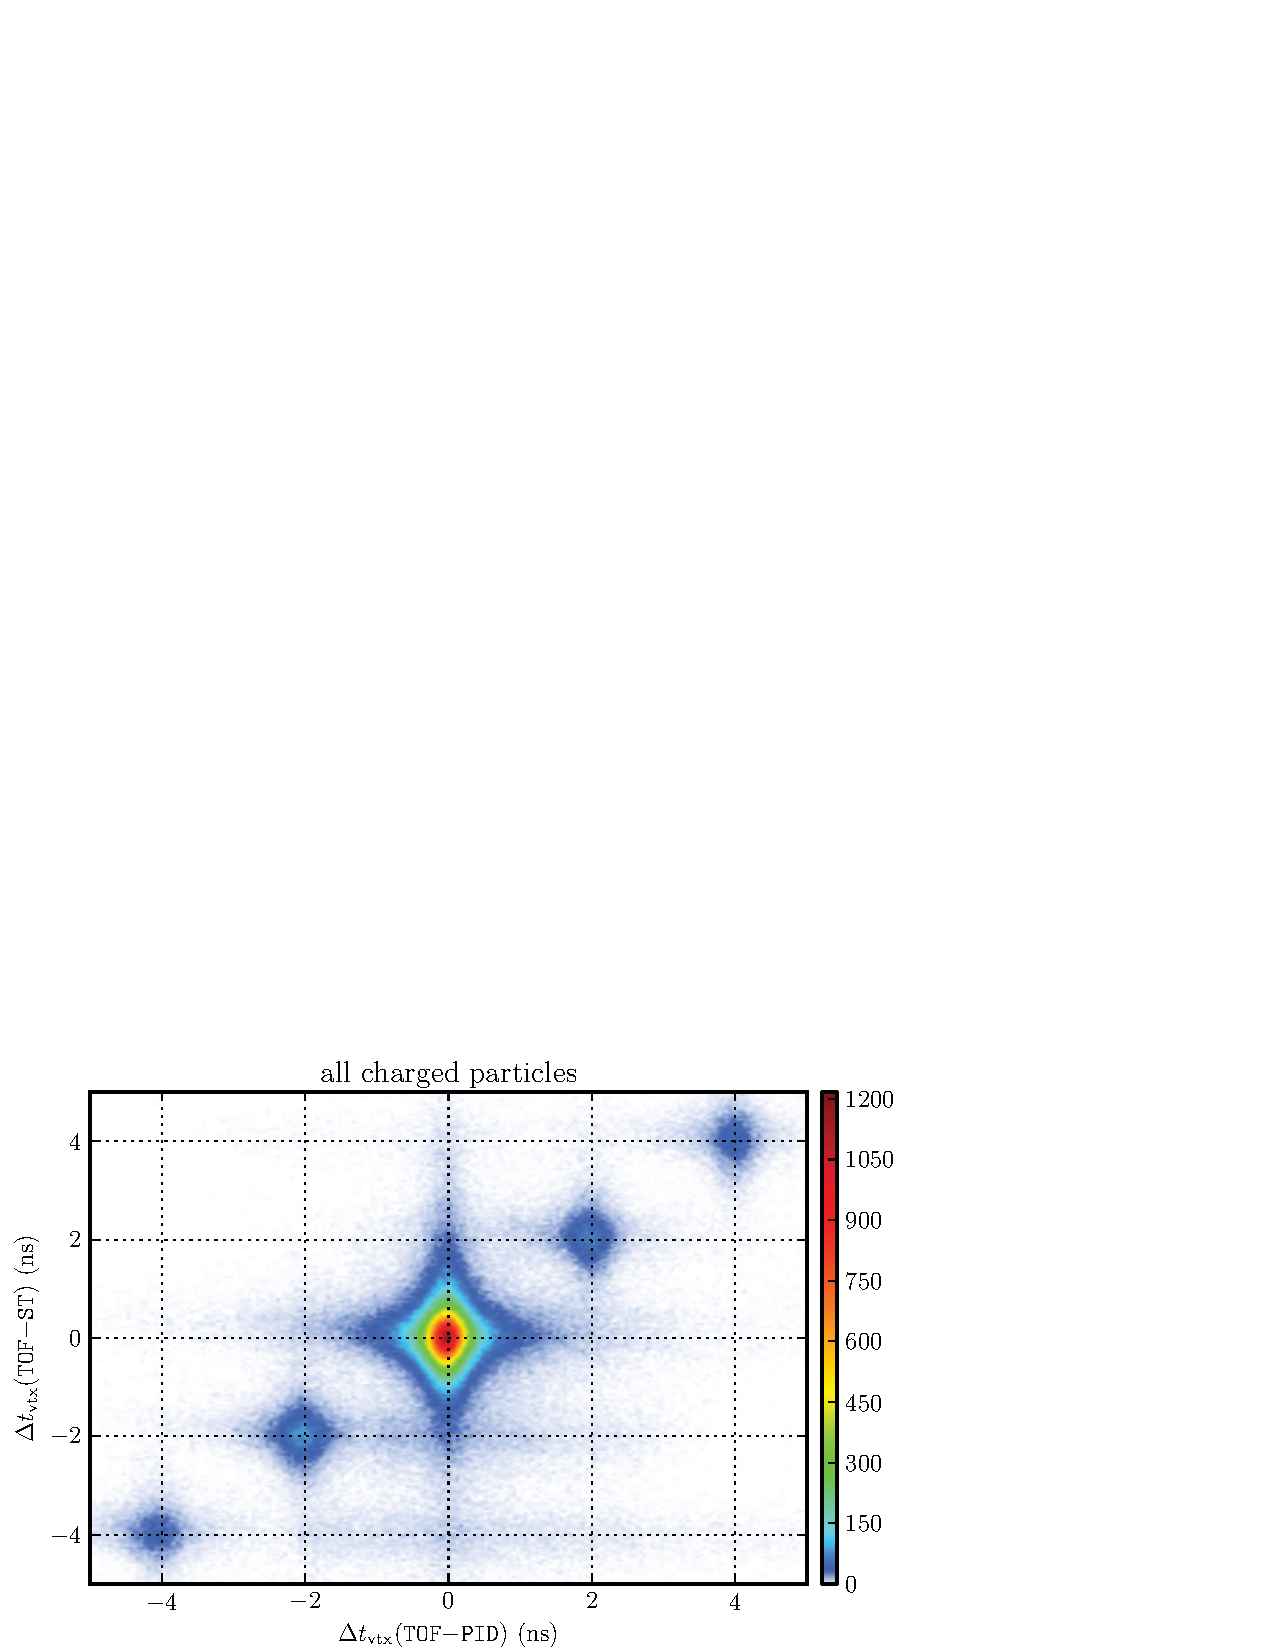
\includegraphics[width=0.5\columnwidth]{figures/calib/st/dvertex_time_pid_st.pdf}
\caption[vertex timing, \abbr{TOF-ST} vs.\ \abbr{TOF-PID}]{\label{fig:dvertex_time_pid_st}Difference in vertex times for each track for the two calculations made above. Represents 1.5\% of the total statistics.}
\end{center}\end{figure}

\begin{figure}[htbp]\begin{center}
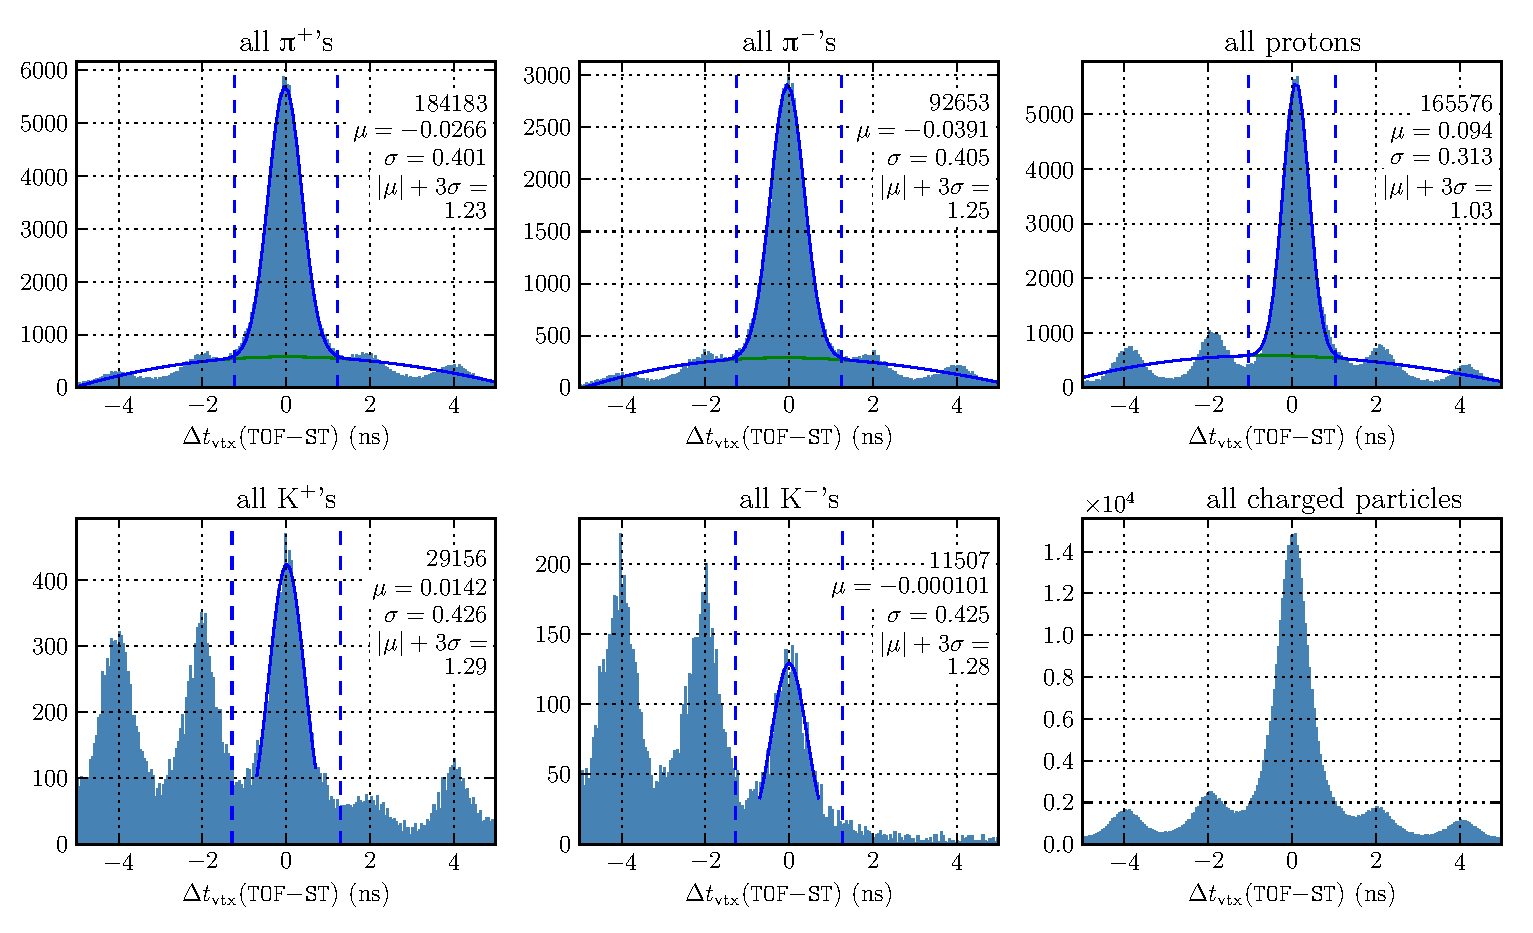
\includegraphics[width=0.9\columnwidth]{figures/calib/st/dvertex_time_st.eps}
\caption[vertex timing, \abbr{TOF-ST}]{\label{fig:dvertex_time_st}Difference in vertex time between that of the photon and of the tracks based on start counter and time-of-flight times. Represents 1.5\% of the total statistics.}
\end{center}\end{figure}


\subsubsection{\label{sec:calib.st.eff}Start Counter Efficiency}

The efficiency of the start counter was calculated by examining the number of tracks with a ST hit after track reconstruction. The ST fired $91.6\%$ of the time, this was calculated from run 57000 since it is a good run and included in production data. This percentage was calculated for the start counter as a whole. Any analysis that uses associated start counter hits with identified tracks must take this efficiency into account. Note, however, that this effect is very small ($< 1 \%$) for many-particle final states where only a single start counter is required.

\FloatBarrier

\subsection{\label{sec:calib.dc}Drift Chamber Calibration and Resolution}

Tracking in the Drift Chamber of a \abbr{CLAS} Sector is performed using the six superlayers of the \abbr{DC}. A good measure of the the quality of tracking are the \abbr{DC} residuals for each superlayer. After a track is identified using the hit elements in the \abbr{DC} superlayer, It's \abbr{DC} residual is calculated using the TBLA bank as follows:

\begin{verbatim}
fabs(TBLA->tbla[i].fitdoca) - fabs(TBLA->tbla[i].calcdoca)
\end{verbatim}

\begin{v2}The Drift Chamber alignment was done by correcting the mean of the residuals and the results are shown in Fig.~\ref{fig:dc.align}.\end{v2}  The values of the \abbr{DC} residuals in the \abbr{CLAS} data are empirically found to be a good fit to a convolution of 2 Gaussians - a narrow Gaussian and a broad Gaussian. During \abbr{DC} calibrations efforts were made to minimize this residual to have maximum reconstruction efficiency. The mean and width of the residuals as a function of superlayer and run number are shown in Figs.~\ref{fig:calib.dc.residuals.mean} and \ref{fig:calib.dc.residuals.wid} respectively.

\begin{figure}\begin{center}
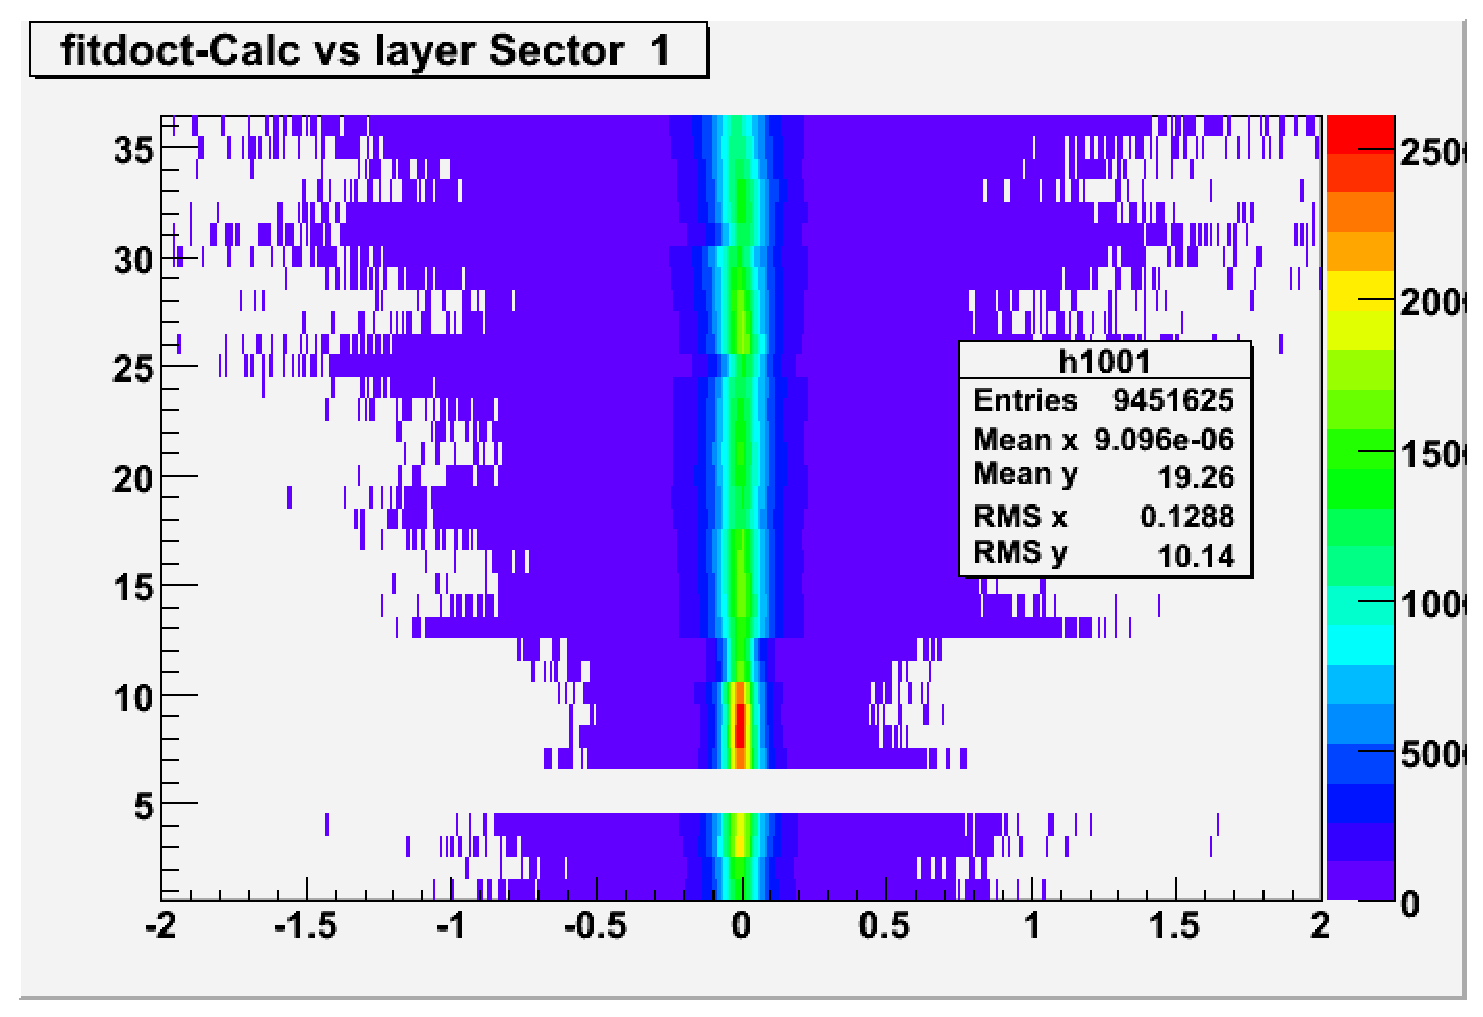
\includegraphics[width=0.6\textwidth]{figures/calib/dc/dc_align1.eps}
\caption[DC Alignment]{\label{fig:dc.align}Alignment of the Drift Chambers in sector 1. All other sectors show very similar results.}
\end{center}\end{figure}

\begin{figure}\begin{center}
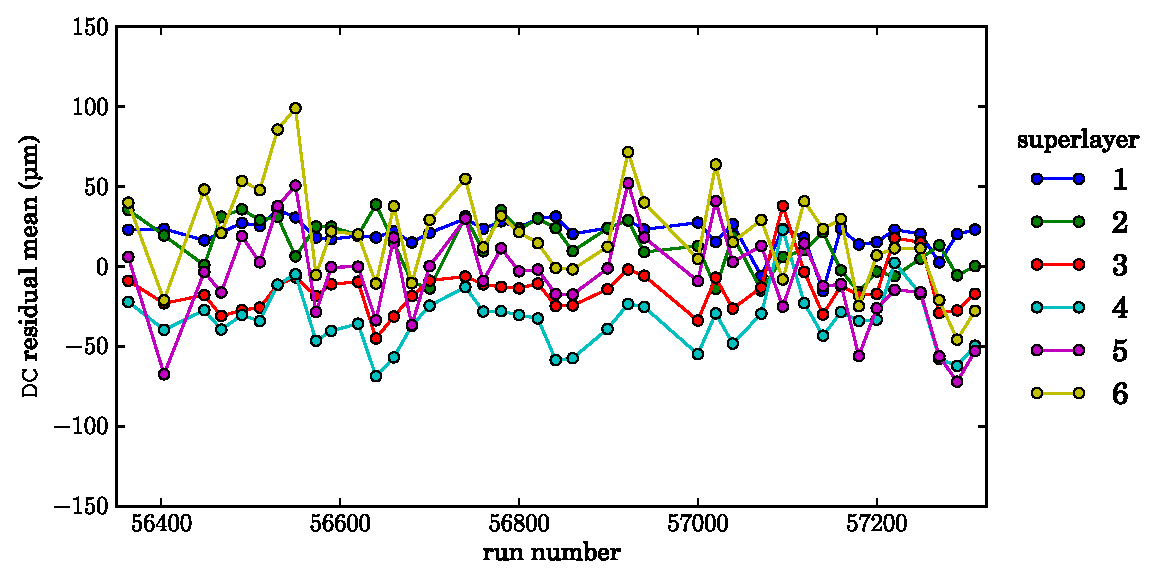
\includegraphics[width=0.6\textwidth]{figures/calib/dc/dc_resid_mean.eps}
\caption[DC Residuals (Mean)]{\label{fig:calib.dc.residuals.mean}Mean of residuals for the drift chambers by superlayer and by run.}
\end{center}\end{figure}

\begin{figure}\begin{center}
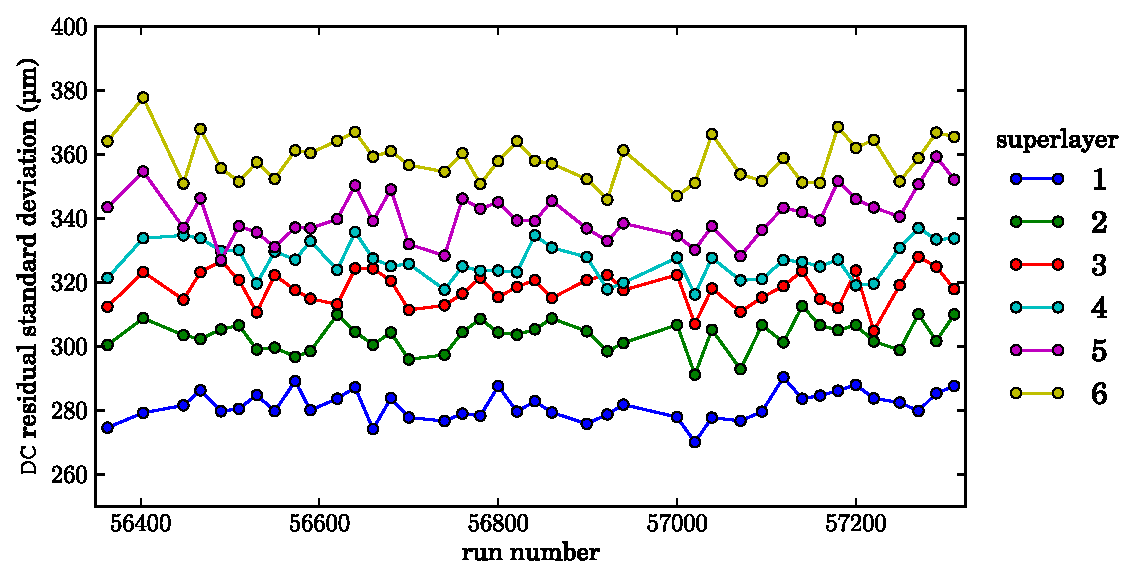
\includegraphics[width=0.6\textwidth]{figures/calib/dc/dc_resid_sigma.eps}
\caption[DC Residuals (Width)]{\label{fig:calib.dc.residuals.wid}Gaussian width of residuals for the drift chambers by superlayer and by run.}
\end{center}\end{figure}

\subsubsection{\label{sec:calib.dc.eff}Drift Chamber Wire Efficiency}

To generate the wire map for \desg{g12}, the utility \prog{pdu}, available in \abbr{SVN}, was used. Maurizio Ungaro made the wire-maps for \desg{g12} with the root files [\verb+A01+ and \verb+A02+] for each run. These output files are at \url{/home/mukesh/work/pdu_hbook} at \abbr{Jlab}. Root files needed are at \url{/home/mukesh/work/pdu_root}. The values were added to the \desg{g12} database. The results of the wire map are plotted in for each sector and can be found here:
\begin{verbatim}
http://www.jlab.org/~ungaro/maureepage/proj/dceff/dc_periods/g12.html
\end{verbatim}
\begin{v2}An example plot from this site is shown in Fig.~\ref{fig:calib.dc.eff}. The DC wire efficiencies were computed for each wire using the whole data set, using the CLAS utility \prog{pdu}. An example of this is shown in the beginning of DC calibration section. Simulation data all use the \prog{gpp} to apply this efficiency map. Comparison of the real data and MC data depends on the topology and model.\end{v2}

\begin{figure}\begin{center}
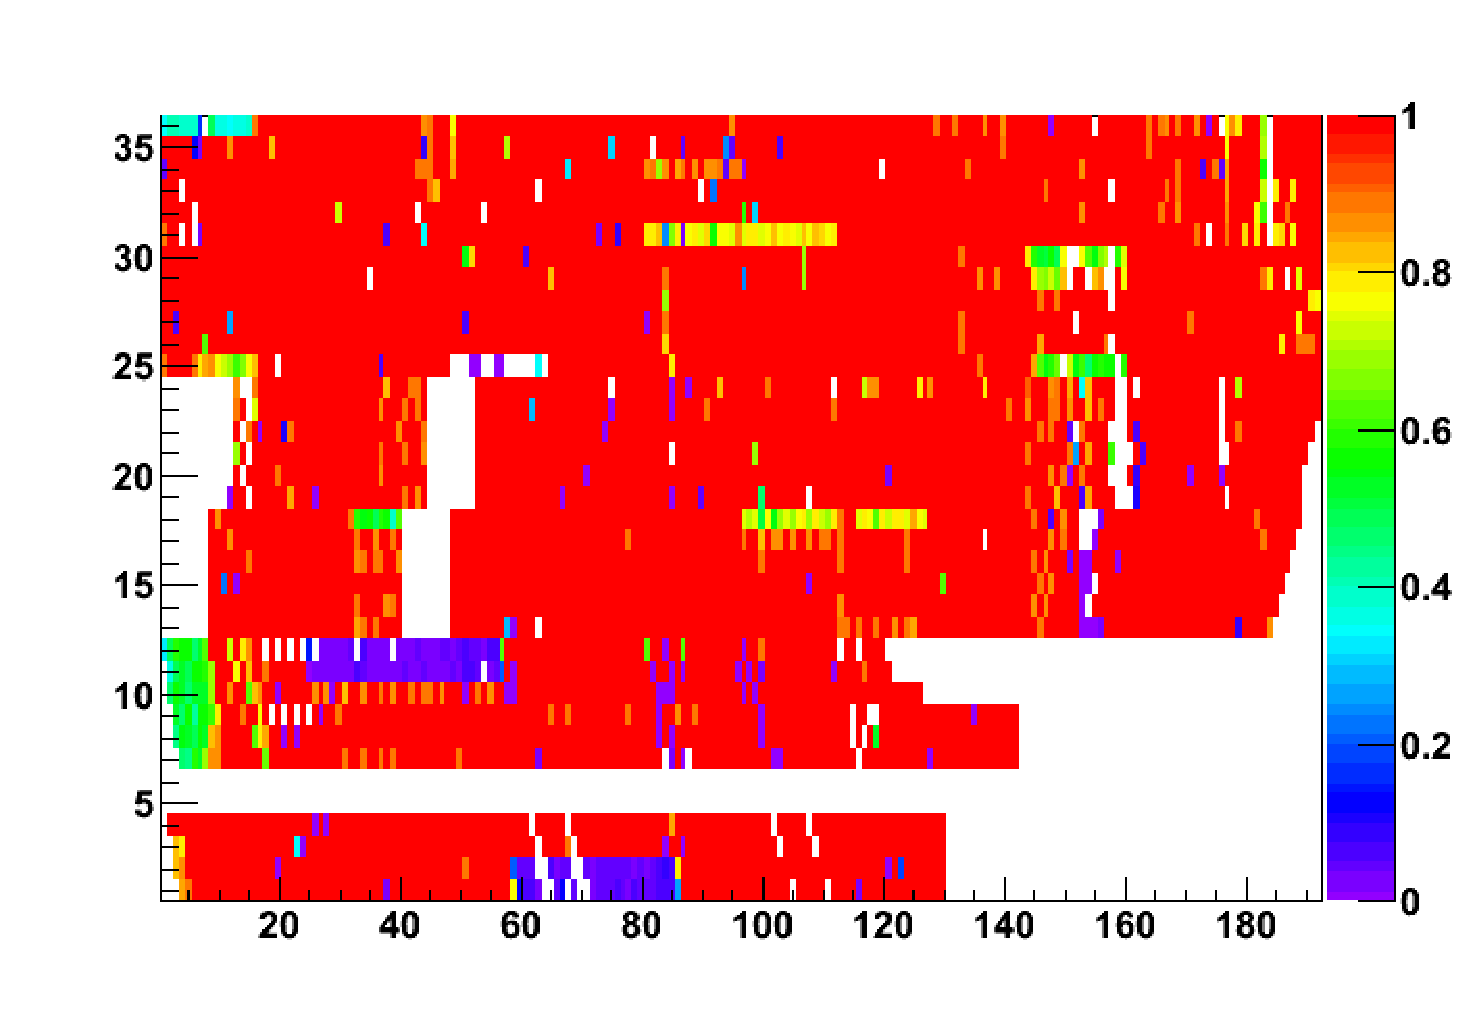
\includegraphics[width=0.6\textwidth]{figures/calib/dc/Occupancy_g12_s1.eps}
\caption[DC Efficiency Map Sector 1]{\label{fig:calib.dc.eff}DC efficiency map for sector 1. All other sectors show very similar results.}
\end{center}\end{figure}

\FloatBarrier


\subsection{\label{sec:calib.cc}Cerenkov Calibration and Performance}

The Cerenkov detector's primary role in CLAS is to help differentiate leptons from pions at momentums below the pion Cerenkov radiation threshold.  The Cerenkov for g12 was roughly calibrated by importing the (then) most recent CLAS CC calibration constants and then verifying that the photoelectron number was reasonable on a sector by sector basis.  The following validation plots come from two g12 production runs skimmed only for pions via the standard PID, and inside the fiducial region as described in this document.  In Fig.~\ref{calib.cc_pesec} the total photoelectron yield for each sector is shown.  The histogram y-axis range is constant between all plots for ease of comparison.  One can see that the photoelectron yield is consistent between sectors.

\begin{figure}[htpb]
\begin{center}
 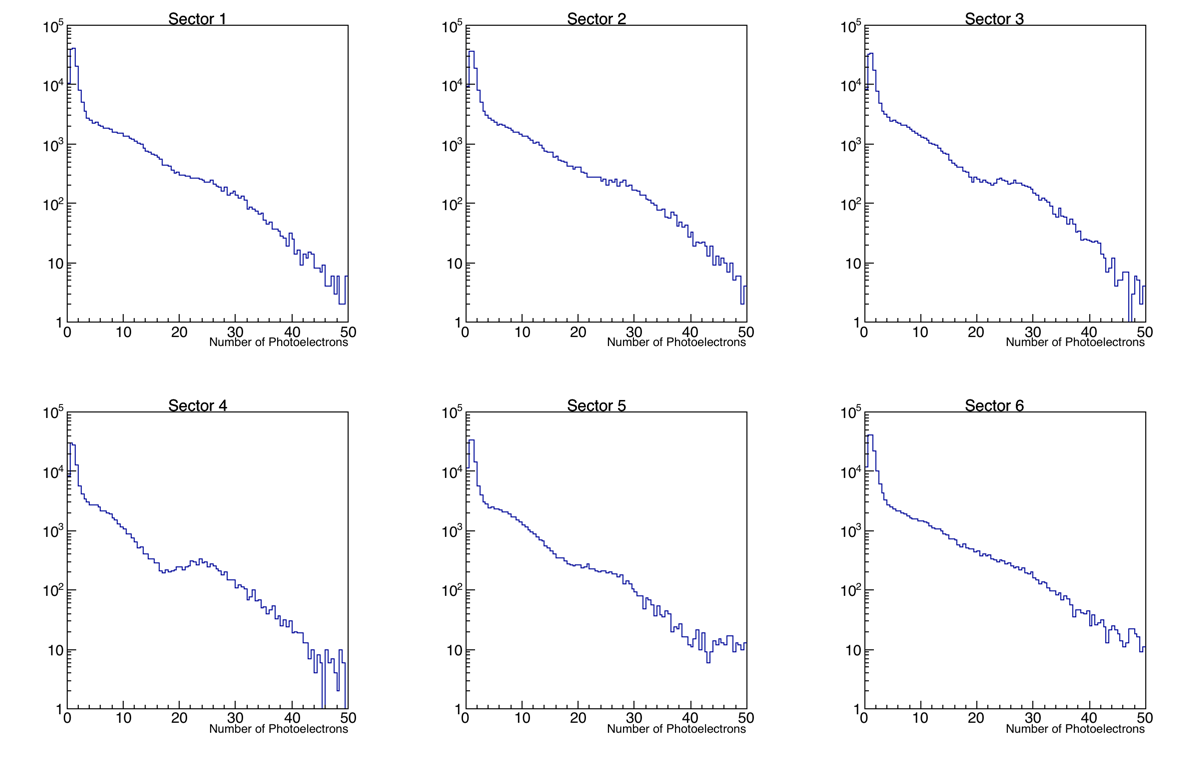
\includegraphics[width=0.75\textwidth]{figures/calib/cc/npeCC_check.png}
  \caption{An example CC photoelectron spectra from two production runs skimmed for pions.  The y-axis range is fixed over all plots for ease of comparison.}
  \label{calib.cc_pesec}
  \end{center}
\end{figure}

In Fig.~\ref{calib.cc_pepmt} the photoelectron yields are further broken down by PMT.  The z-axis (log-scale) is fixed for ease of comparison.  The important feature here is that the delta-ray "pion" peak in the photoelectron spectra peaks roughly around 1.0 photoelectrons for all PMTs. The general lepton selection criteria includes a cut > 2.5 photoelectrons, which is a relatively safe and conservative cut on any PMT (see Sec.~\ref{sec:data.lepton} for more details on the lepton PID).

\begin{figure}[htpb]
\begin{center}
 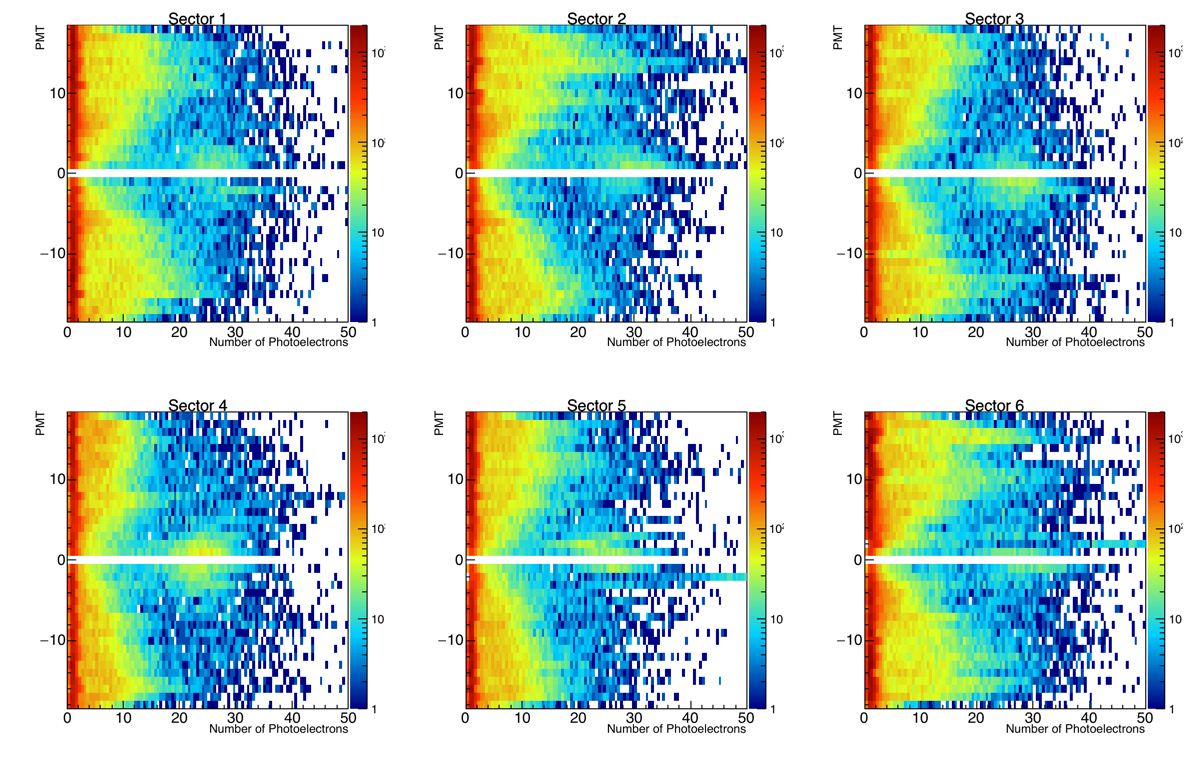
\includegraphics[width=0.75\textwidth]{figures/calib/cc/PMT_v_npe_log.png}
  \caption{Same plot as Fig.~\ref{calib.cc_pesec} but 2D in PMT number.  Negative and positive PMT numbers correspond to left and right CC PMTs. Z-axis range is fixed for ease of comparison.}
  \label{calib.cc_pepmt}
  \end{center}
\end{figure}

As an additional validity plot, the probability of a pion to cause a hit in the CC versus the momentum of the pion is shown in Fig.~\ref{calib.cc_piprob}.  This plot shows the expected behavior of the CC as the pions passes the Cerenkov radiation threshold.

\begin{figure}[htpb]
\begin{center}
 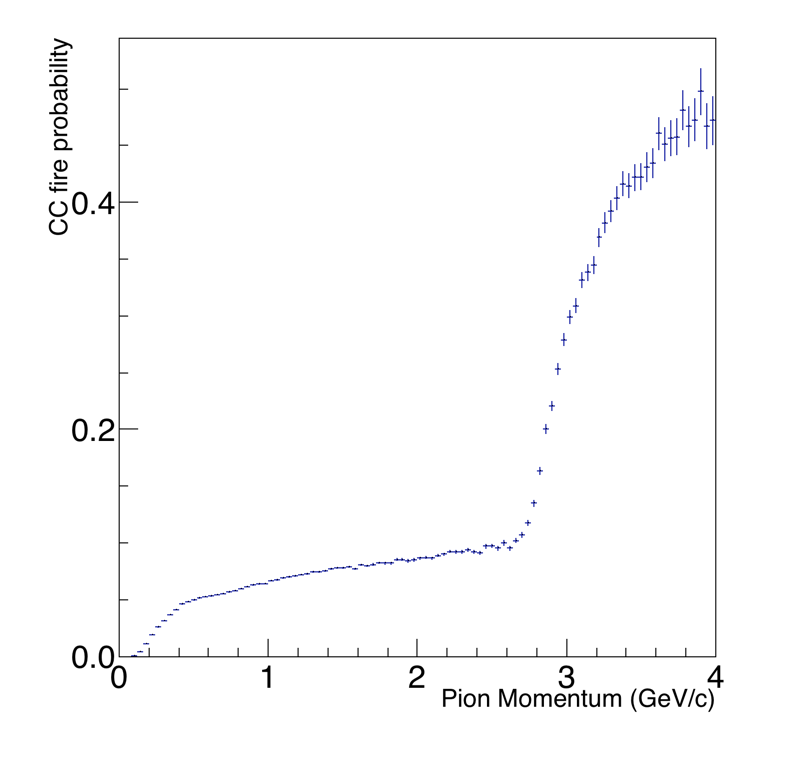
\includegraphics[width=0.45\textwidth]{figures/calib/cc/pionProb.png}
  \caption{The overall CC hit probability for pions within the fiducial region versus the pion momentum.}
  \label{calib.cc_piprob}
  \end{center}
\end{figure}

\subsubsection{\label{sec:calib.cc.eff}Cerenkov Efficiency}
The exact efficiency of the CC over all momenta and angles for leptons was never explicitly calculated.  Instead, it is recommended to look at the efficiency of the overall lepton identification procedure, if needed, for any lepton analyses.


\FloatBarrier

\subsection{\label{sec:calib.tof}Time-of-Flight Counter Calibration and Resolution}

\subsubsection{\label{sec:calib.tof.eff}Time-of-Flight Counter Efficiency and Bad Paddles}

As a standard procedure of the time-of-flight calibrations, the time-of-flight scintillators were initially studied during the calibration period, in which a list~\footnote{Can be obtained using the CLAS calibration database} of scintillators had a faulty ADC or TDC as shown in \ref{tab:craigtof}. Another study, as shown below, was conducted to determine the efficiency of each paddle and to reevaluate the status of their ADC and TDC. Due to the more stringent requirements of paddle efficiency in the study below, more paddles were considered to be faulty than in the initial study. \ref{tab:diff} shows the additional paddles which were considered to be inefficient.

\begin{table}
\begin{minipage}{\textwidth}
\begin{center}
\begin{singlespacing}

\caption{\label{tab:craigtof}List of faulty paddles as compiled during calibration}
    
\begin{tabular}{llp{.43\textwidth}}

\hline \hline

Sector & SCID & Notes \\

\hline

1 & 6 & No ADCR and TDCR \\
2 & 8 & No ADCL and TDCL \\
2 & 34 & No ADCL and TDCL \\
3 & 11 & No ADCR and TDCR \\
3 & 57 & No ADCL, ADCR, TDCL, and TDCR \\
4 & 48 & No ADCL and TDCL \\
5 & 57 & No ADCL, ADCR, TDCL, and TDCR \\
6 & 5 & No ADCR and TDCR \\

\hline \hline

\end{tabular}

\end{singlespacing}
\end{center}
\end{minipage}
\end{table}
 % label: tab:craigtof

\begin{figure}
    %\vspace{16pt}
    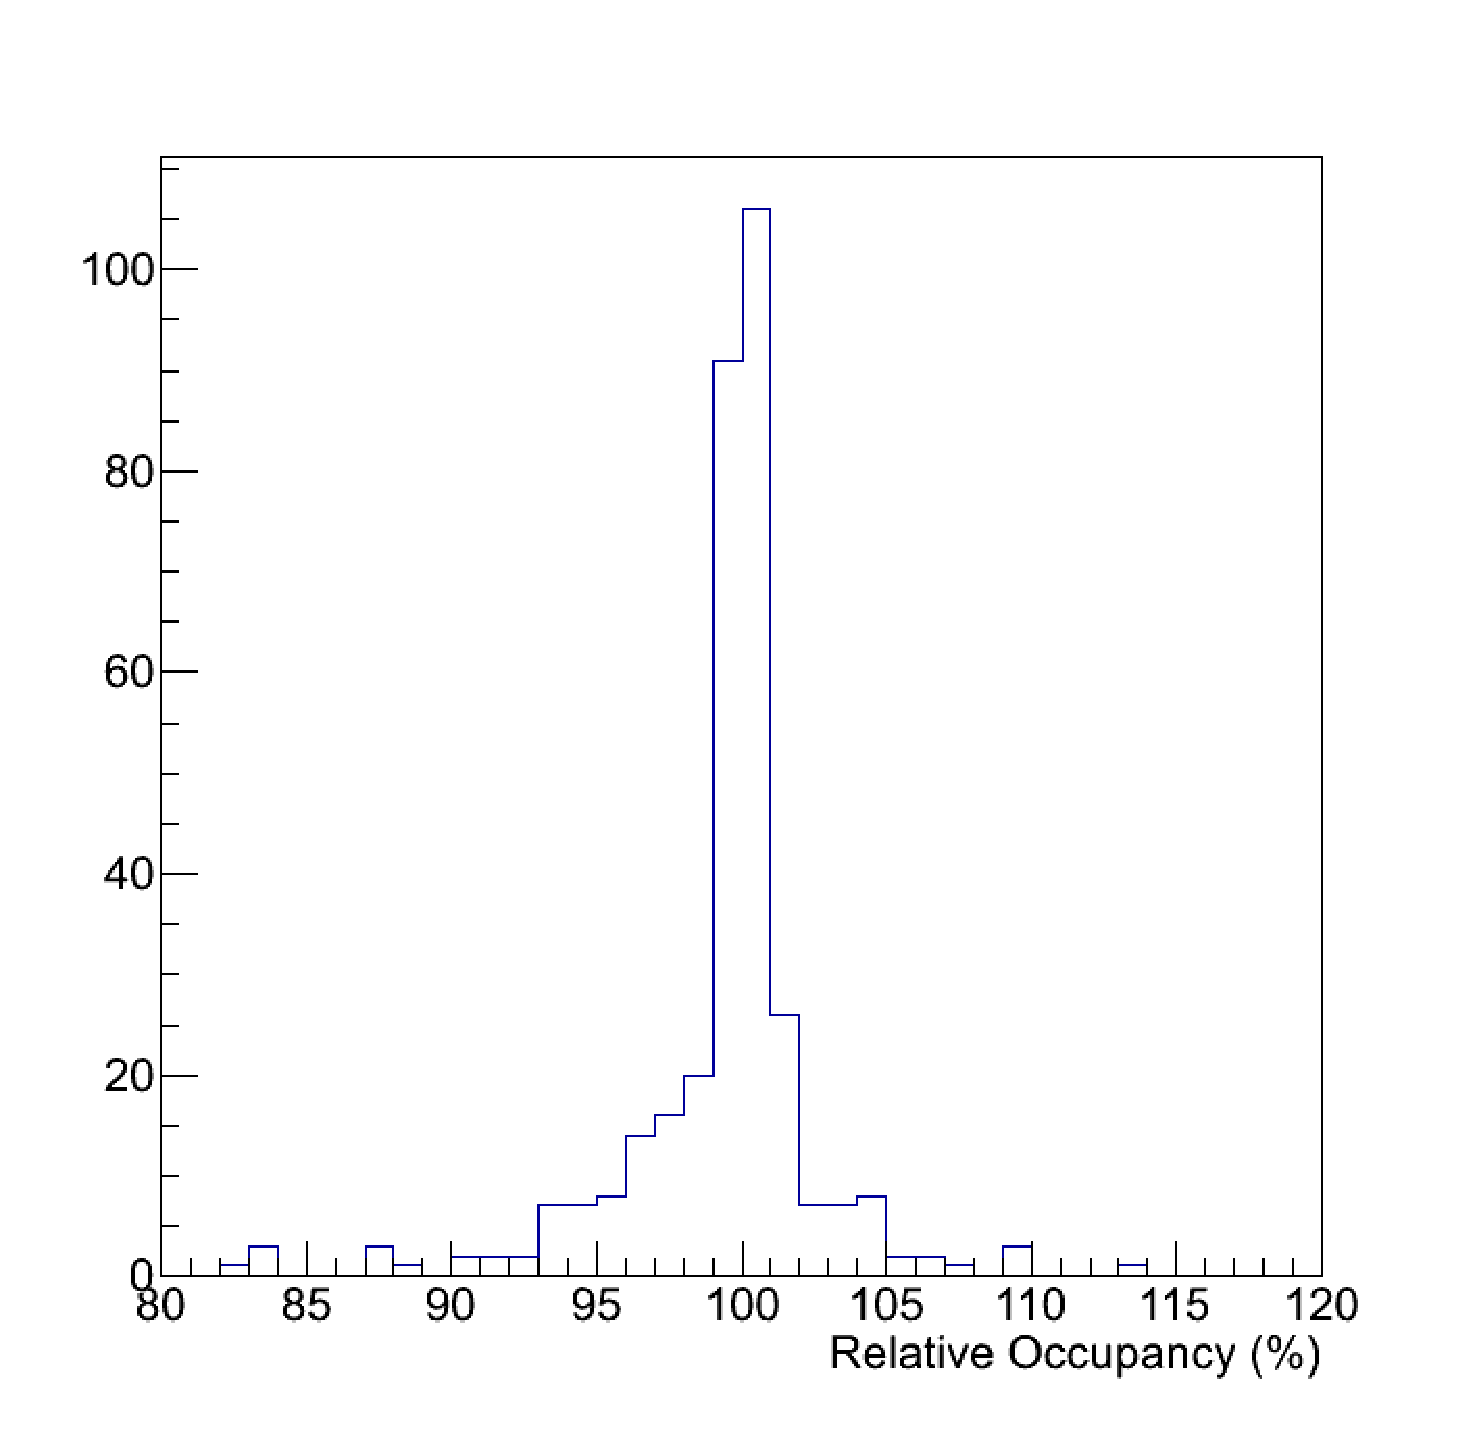
\includegraphics[trim=0 40 10 40,clip,width=.70\linewidth]{figures/calib/tof/tofko/occp.eps}
    \caption{Relative occupancy of all scintillators}
    \label{plt:occp}
\end{figure}

To determine efficiency of each scintillator paddle, the number of hits~\footnote{The data used were obtained from the \texttt{clas\underline{\hspace{5pt}}0$[$run\#$]$.A01} files located in \texttt{$/$mss$/$clas$/$g12$/$data$/$}} registered by every paddle was recorded~\footnote{This was done by using \texttt{bosdump -GSC} and parsing its output}. The relative occupancy of paddle $i$ in sector $j$ is defined the following way: list the number of hits recorded by all paddle $i$'s in sectors $\neq j$ and remove the ones with the most and least hits from the list. Take the average number of hits of the remaining three paddles. The relative occupancy is defined as 
\[
100 \times \frac{ \mathrm{Number of hits in paddle } i \mathrm{ of sector } j}{\mathrm{Average of remaining three paddles}} \hspace{2pt}\%
\]

\ref{plt:occp} shows the relative occupancy of all scintillators plotted on a single histogram. A paddle is defined as inefficient if it is greater than two standard deviations below the mean relative occupancy of all scintillators. \ref{tab:occp} shows the paddles which are below two (left) or three (right) standard deviations below the mean relative occupancy.


\input{tables/tof_padpaddles_stddev} % label: tab:occp

\subsubsection{ADC and TDC Values}


\begin{figure}
    %\vspace{-16pt}
    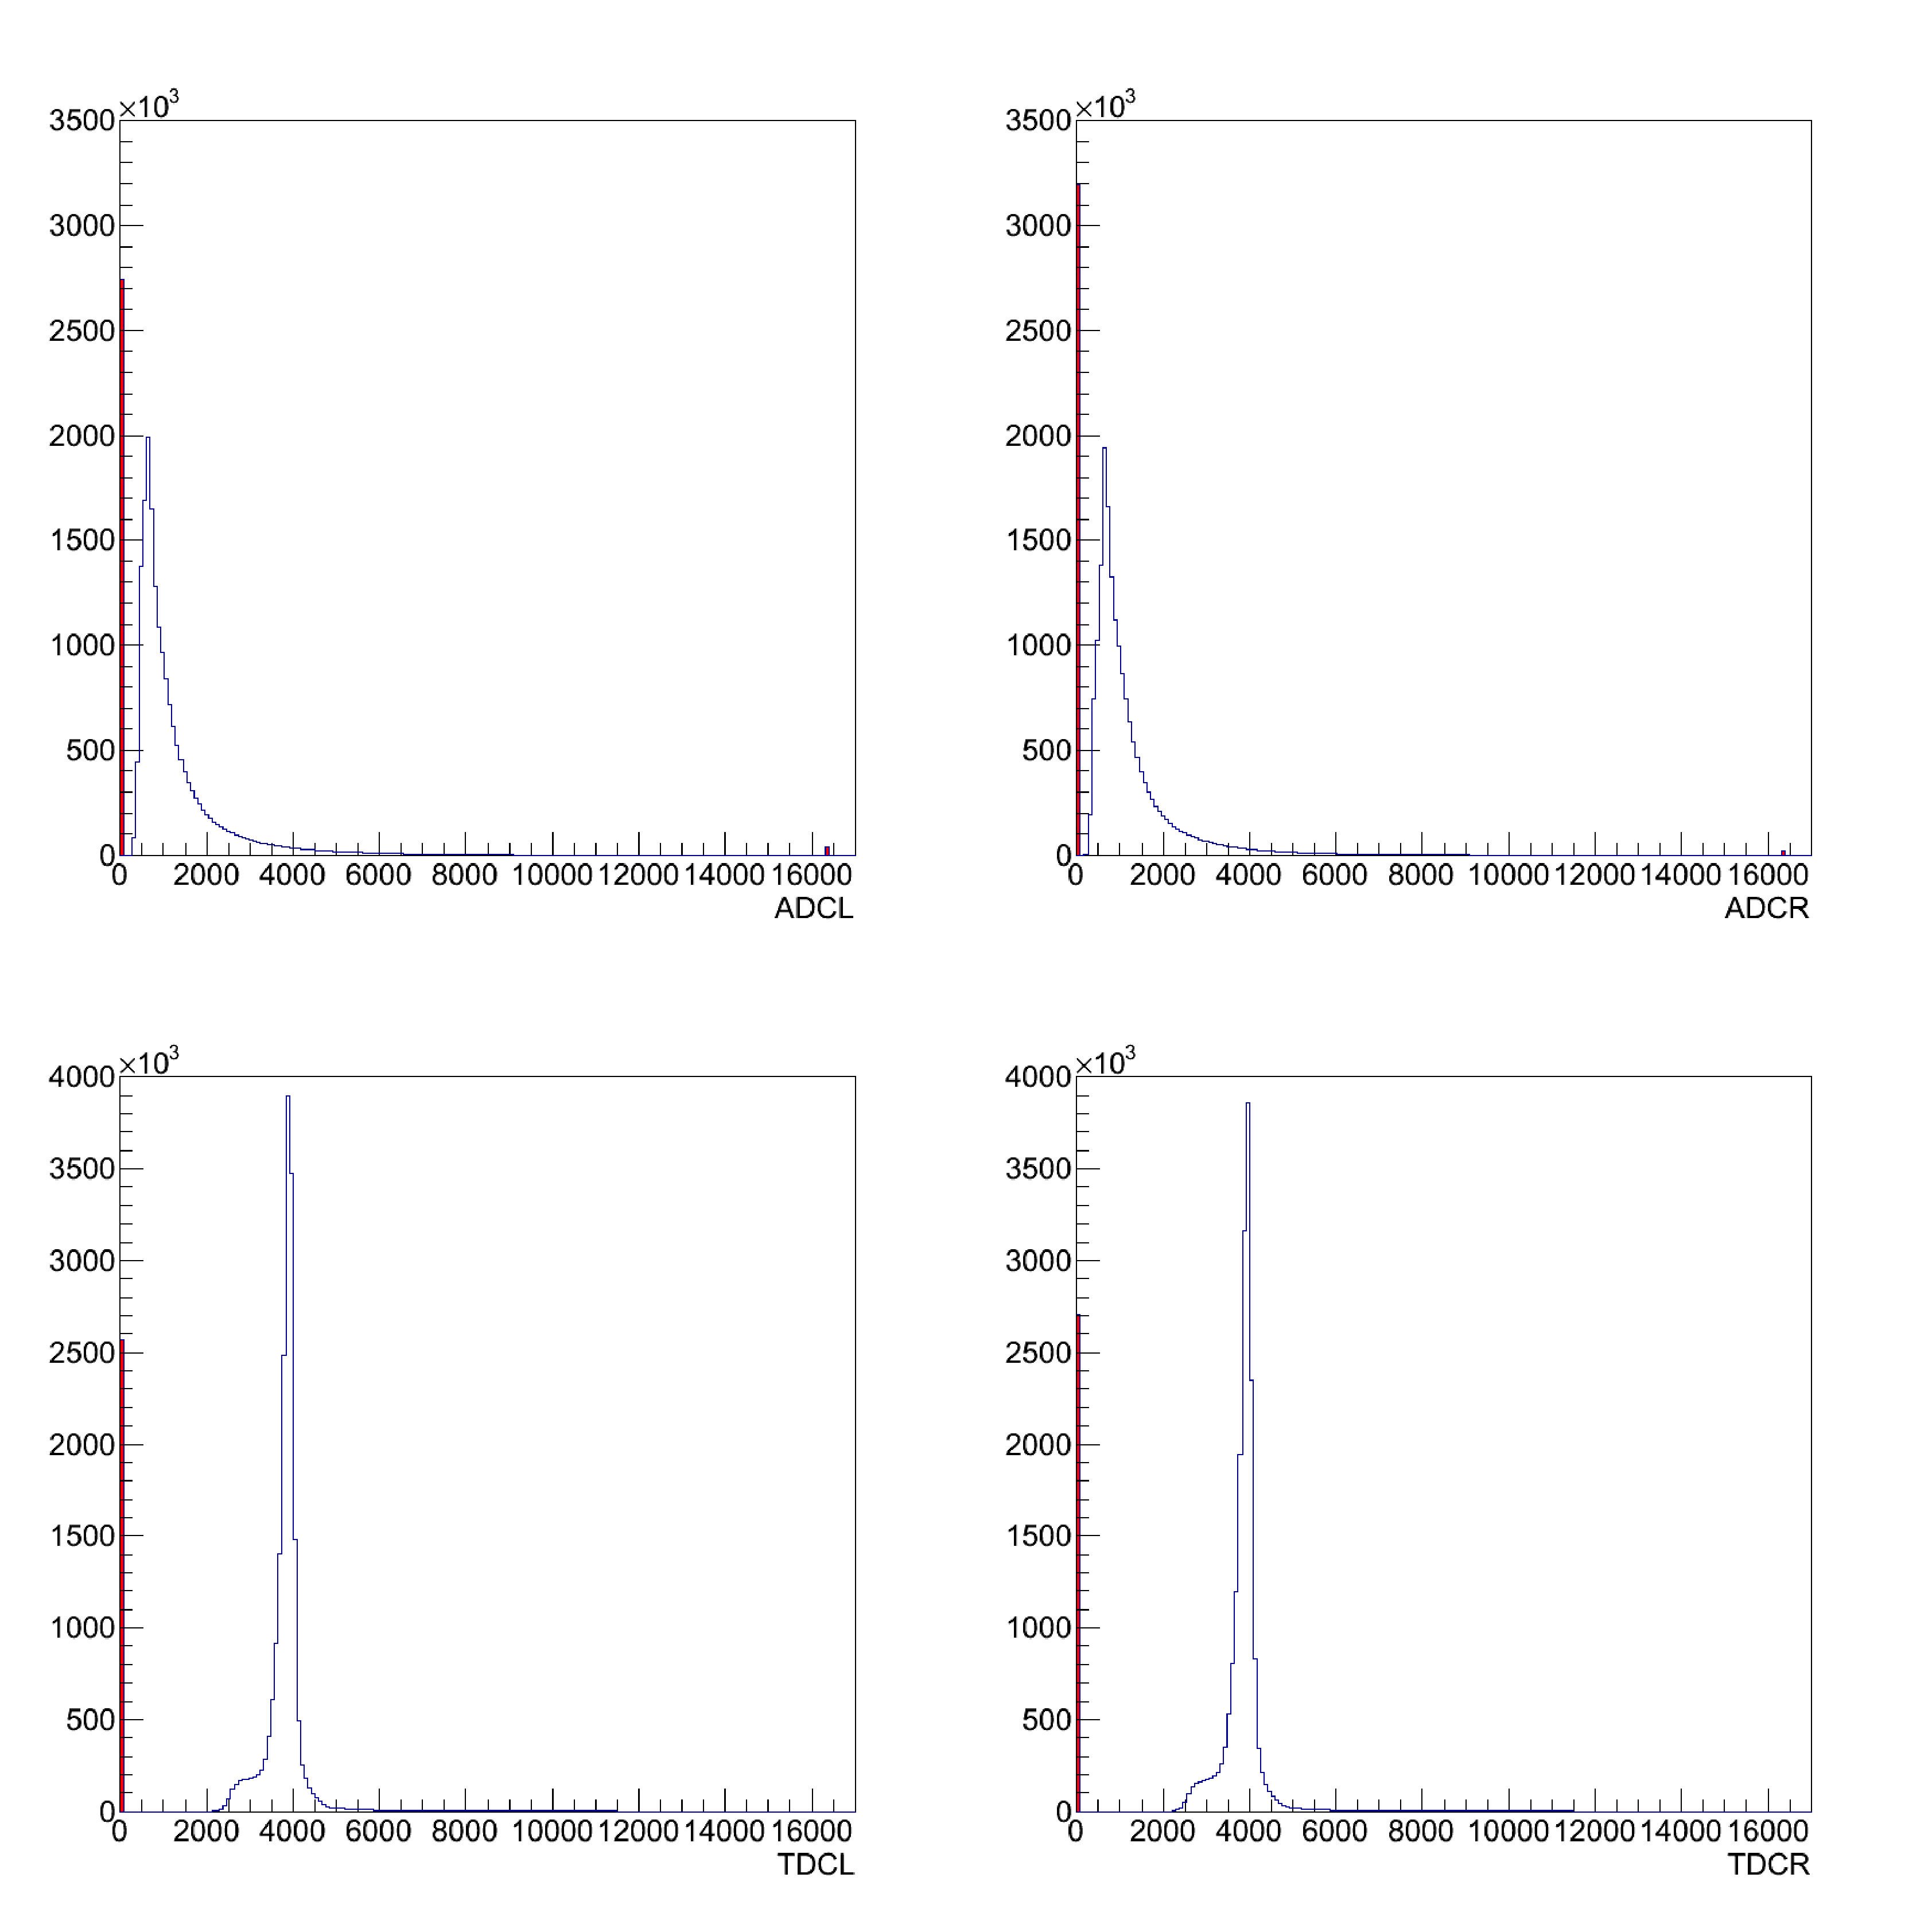
\includegraphics[width=0.70\linewidth]{figures/calib/tof/tofko/adctdcval.eps}
    \caption{Top: ADC values of all scintillators. Left ADC (ADCL) values are on the left and right ADC values are on the right (ADCR). Shaded in red are events recorded with an ADC value of zero or maximum. Bottom: Same as Top but for TDC values}
    \label{plt:adctdcval}
\end{figure}


The occupancy alone is not enough to determine which scintillators are bad. The ADC and TDC values for all scintillators were also recorded and studied. \ref{plt:adctdcval} shows the ADC and TDC values for all scintillators. Some of the events registered had an ADC or TDC value of zero or a maximum ADC value (shaded in red). The percentage of events a scintillator recorded either a TDC or ADC value of zero or maximum ADC value was studied as shown in \ref{plt:adc0vSCID,plt:adcMvSCID,plt:tdc0vSCID}. \ref{plt:adc0vSCID,plt:tdc0vSCID,plt:proj} assisted in determining bad paddles. It (is to be) was decided that a paddle cannot have more than $50\%$ of its ADC (left or right) values be equal to zero or more than $45\%$ of its TDC (left or right) values equal to zero. \ref{tab:adctdc0} shows which paddles fall in these categories. \ref{tab:tofko} shows which scintillators should be knocked out due to low occupancy or too many null ADC or TDC values. Due to the small number of events in which a maximum ADC value is obtained, it is not recommended in knocking paddles out based on this measure. However, \ref{tab:adcM} shows the paddles which attain a maximum ADC value on more than $2.5\%$ of its registered events.


\begin{table}
\begin{minipage}{\textwidth}
\begin{center}
\begin{singlespacing}

\caption{\label{tab:adctdc0}Paddles which registered an ADC or TDC value of zero greater than 50\% and 45\%, respectively, of its entries}

\begin{tabular}{lp{.43\textwidth}p{.43\textwidth}}

\hline \hline

 &  \% Events with ADCL or ADCR = 0 \( > \) 50\% &  \% Event with TDCL or TDCR = 0 \( > \) 45\% \\
 
\hline

Sector 1 & 6 (100\% ADCR) & 6 (100\% TDCR), 46 (97.89\% TDCL), 50 (98.11\% TDCL) \\
Sector 2 & 8 (100\% ADCL), 34 (100\% ADCL), 44 (50.22\% ADCL), 54 (52.00\% ADCR) &  8 (100\% TDCL), 34 (100\% TDCL), 44 (47.51\% TDCL), 54 (47.10\% TDCR)\\
Sector 3 & 11 (100\% ADCR), 56 (74.75\% ADCR) & 11 (100\% TDCR), 56 (62.79\% TDCR)\\
Sector 4 & 48 (100\% ADCL) & 48 (100\% TDCL) \\
Sector 5 & 48 (77.98\% ADCL) & 48 (76.10\% TDCL)\\
Sector 6 & 5 (100\% ADCR), 56 (59.30\% ADCR) & 1 (98.78\% TDCL), 5 (100\% TDCR), 33 (97.78\% TDCL) \\

\hline \hline

\end{tabular}

\end{singlespacing}
\end{center}
\end{minipage}
\end{table}
 % label: tab:adctdc0

\begin{table}
\begin{minipage}{\textwidth}
\begin{center}
\begin{singlespacing}

\caption{\label{tab:tofko}Union of \ref{tab:occp,tab:adctdc0} (Recommended list of paddles to knockout)}

\begin{tabular}{lc}

\hline \hline

Sector 1: & 6, 35, 40, 41, 50, 56\\
Sector 2: & 2, 8, 34, 35, 41, 44, 50, 54, 56\\
Sector 3: & 11, 35, 40, 41, 56\\
Sector 4: & 41, 48 \\
Sector 5: & 48\\
Sector 6: & 1, 5, 33, 56 \\

\hline \hline

\end{tabular}

\end{singlespacing}
\end{center}
\end{minipage}
\end{table}

 % label: tab:tofko


\begin{table}
\centering
\begin{tabular}{l | c |}
Sector 1 & 35, 40, 41, 50, 56 \\
Sector 2 & 2, 35, 41, 44, 50, 54, 56 \\
Sector 3 & 35, 40, 41, 56 \\
Sector 4 & 41 \\
Sector 5 & 48 \\
Sector 6 & 1, 33, 56
\end{tabular}
\caption{Paddles in \ref{tab:tofko} not included in \ref{tab:craigtof}}
\label{tab:diff}
\end{table}

\begin{table}
\centering
\begin{tabular}{l | c |}
Sector 1 & 20 (2.93\% ADCL)\\
Sector 3 & 20 (4.26\% ADCL)
\end{tabular}
\caption{Paddles with percentage of hits registering a maximum ADC value \( > \) 2.5\% of its events}
\label{tab:adcM}
\end{table}

\begin{figure}
    %\vspace{-16pt}
    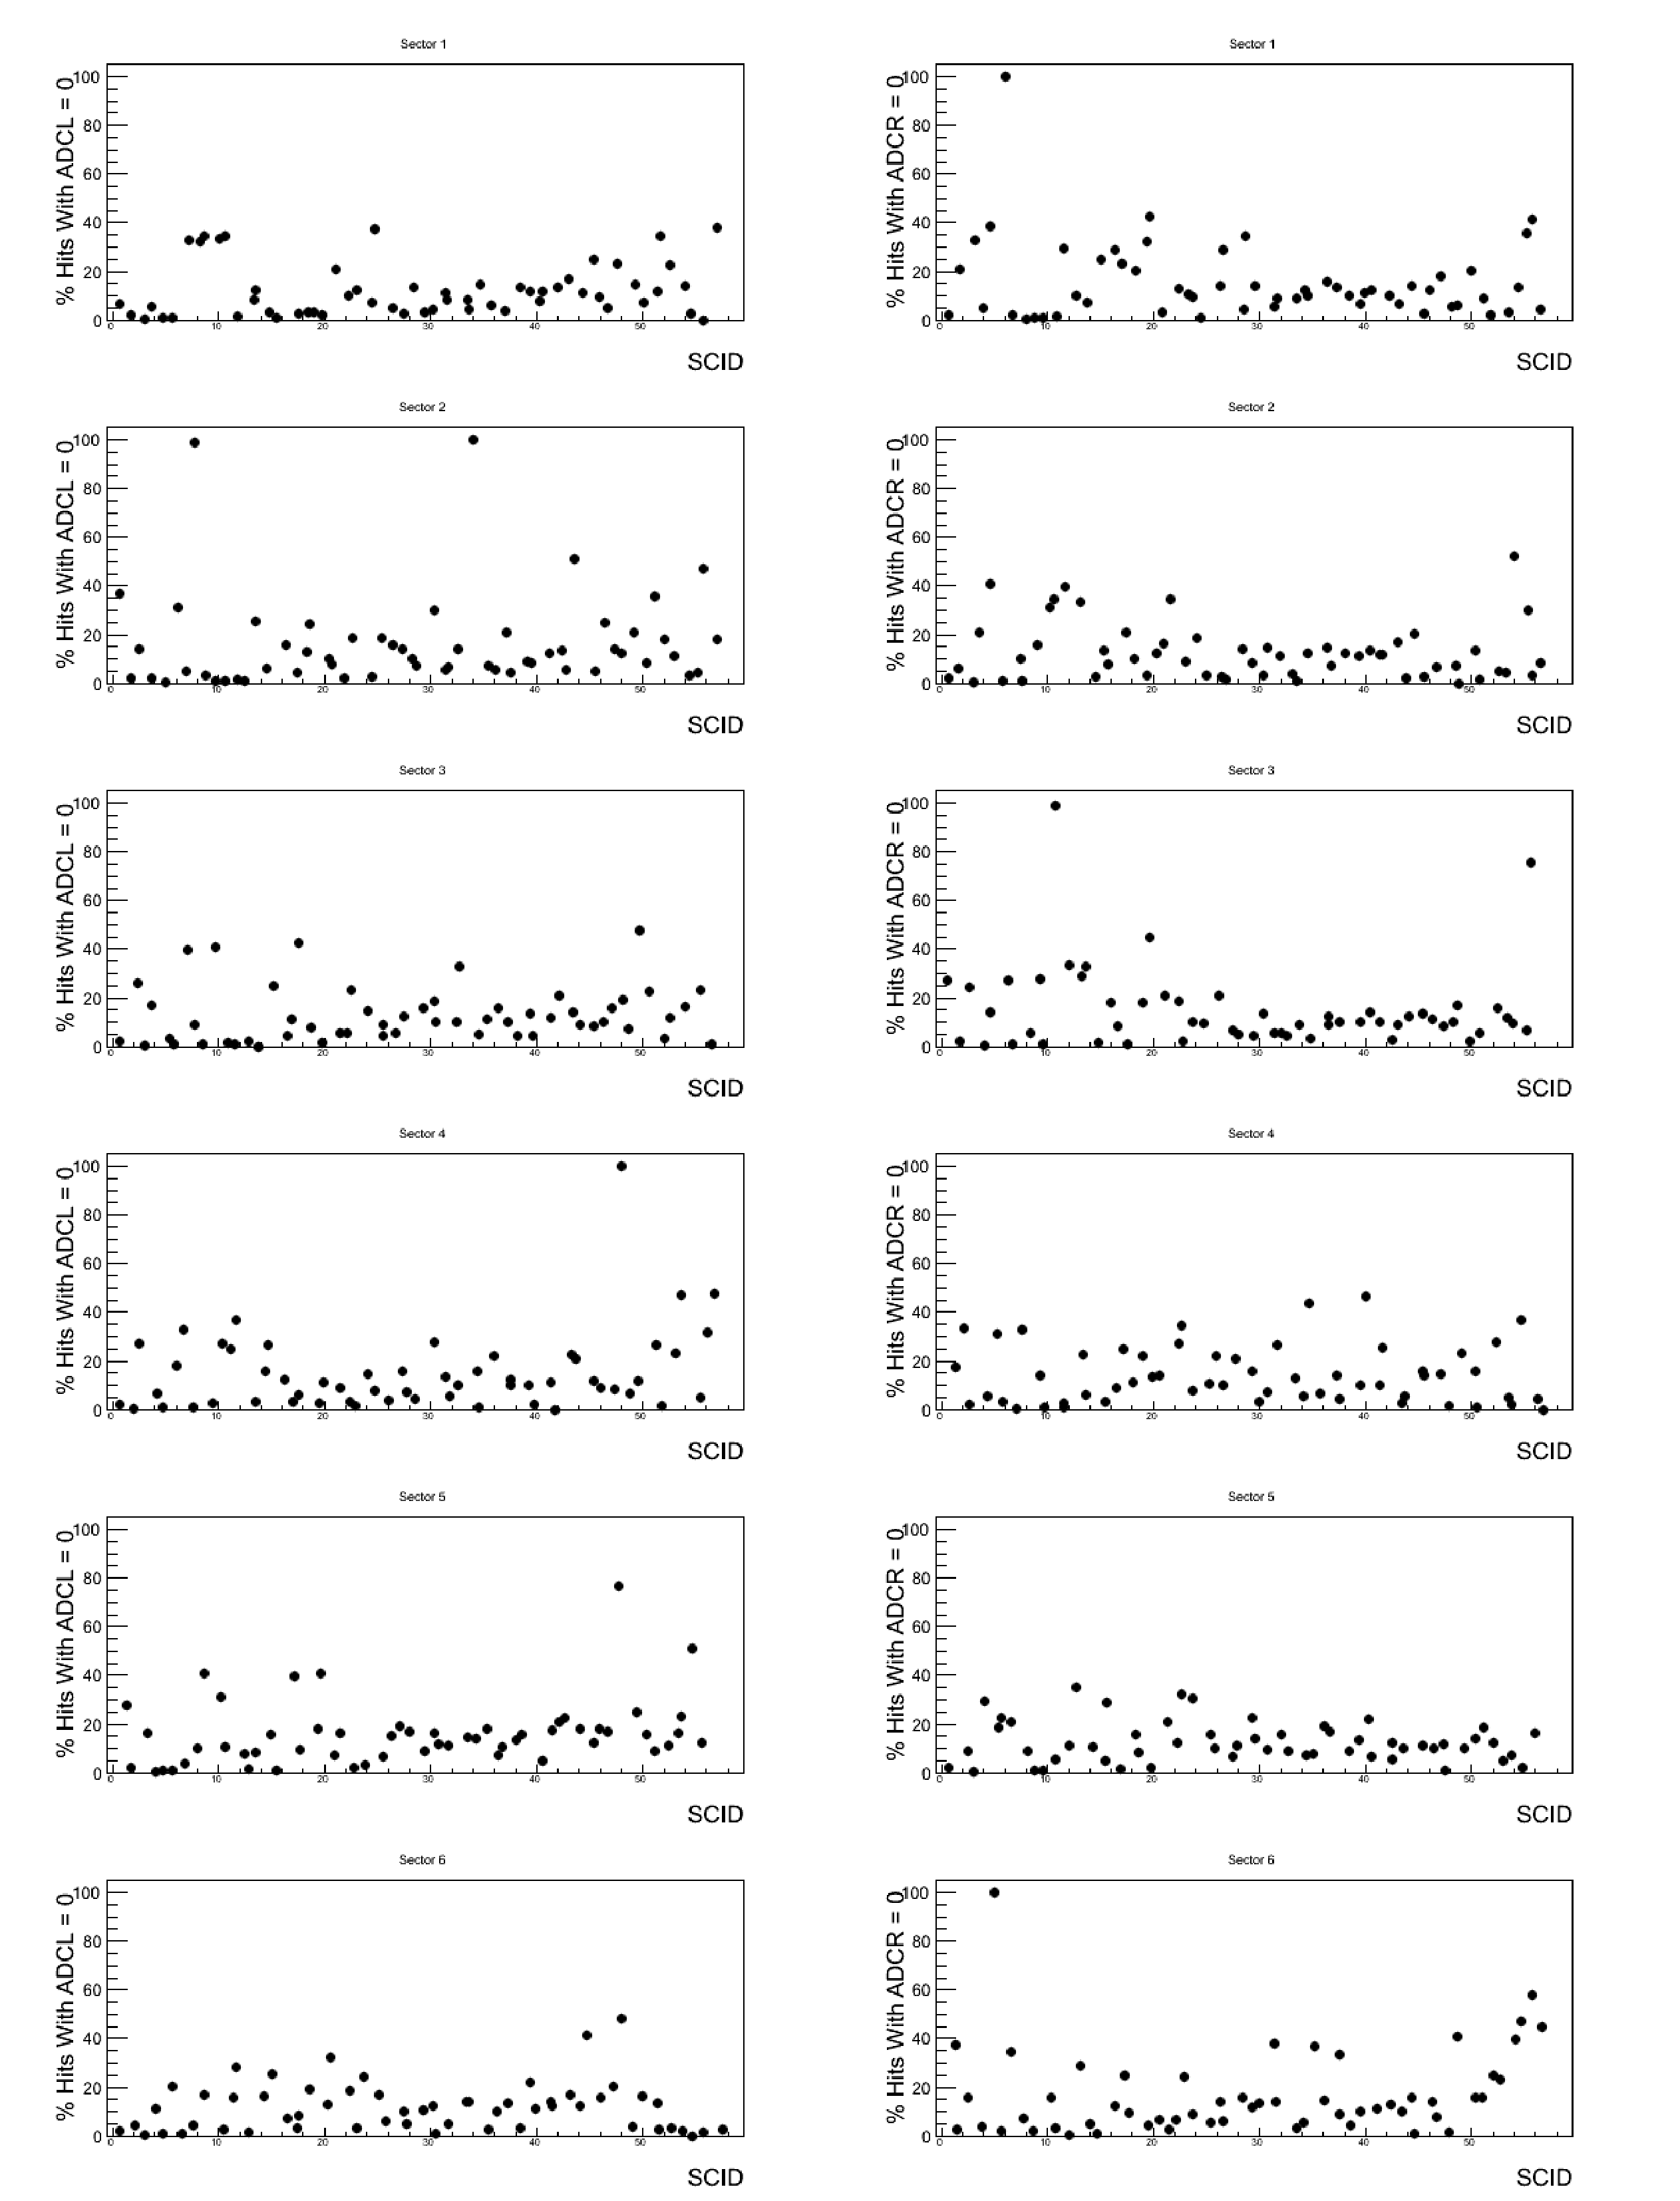
\includegraphics[width=0.8\textwidth]{figures/calib/tof/tofko/adc.eps}
    \caption{Percentage of hits registering an ADC value of 0 for all scintillators. Left ADC (ADCL) are on the left and right ADC (ADCR) values are on the right}
    \label{plt:adc0vSCID}
\end{figure}

\begin{figure}
    %\vspace{-16pt}
    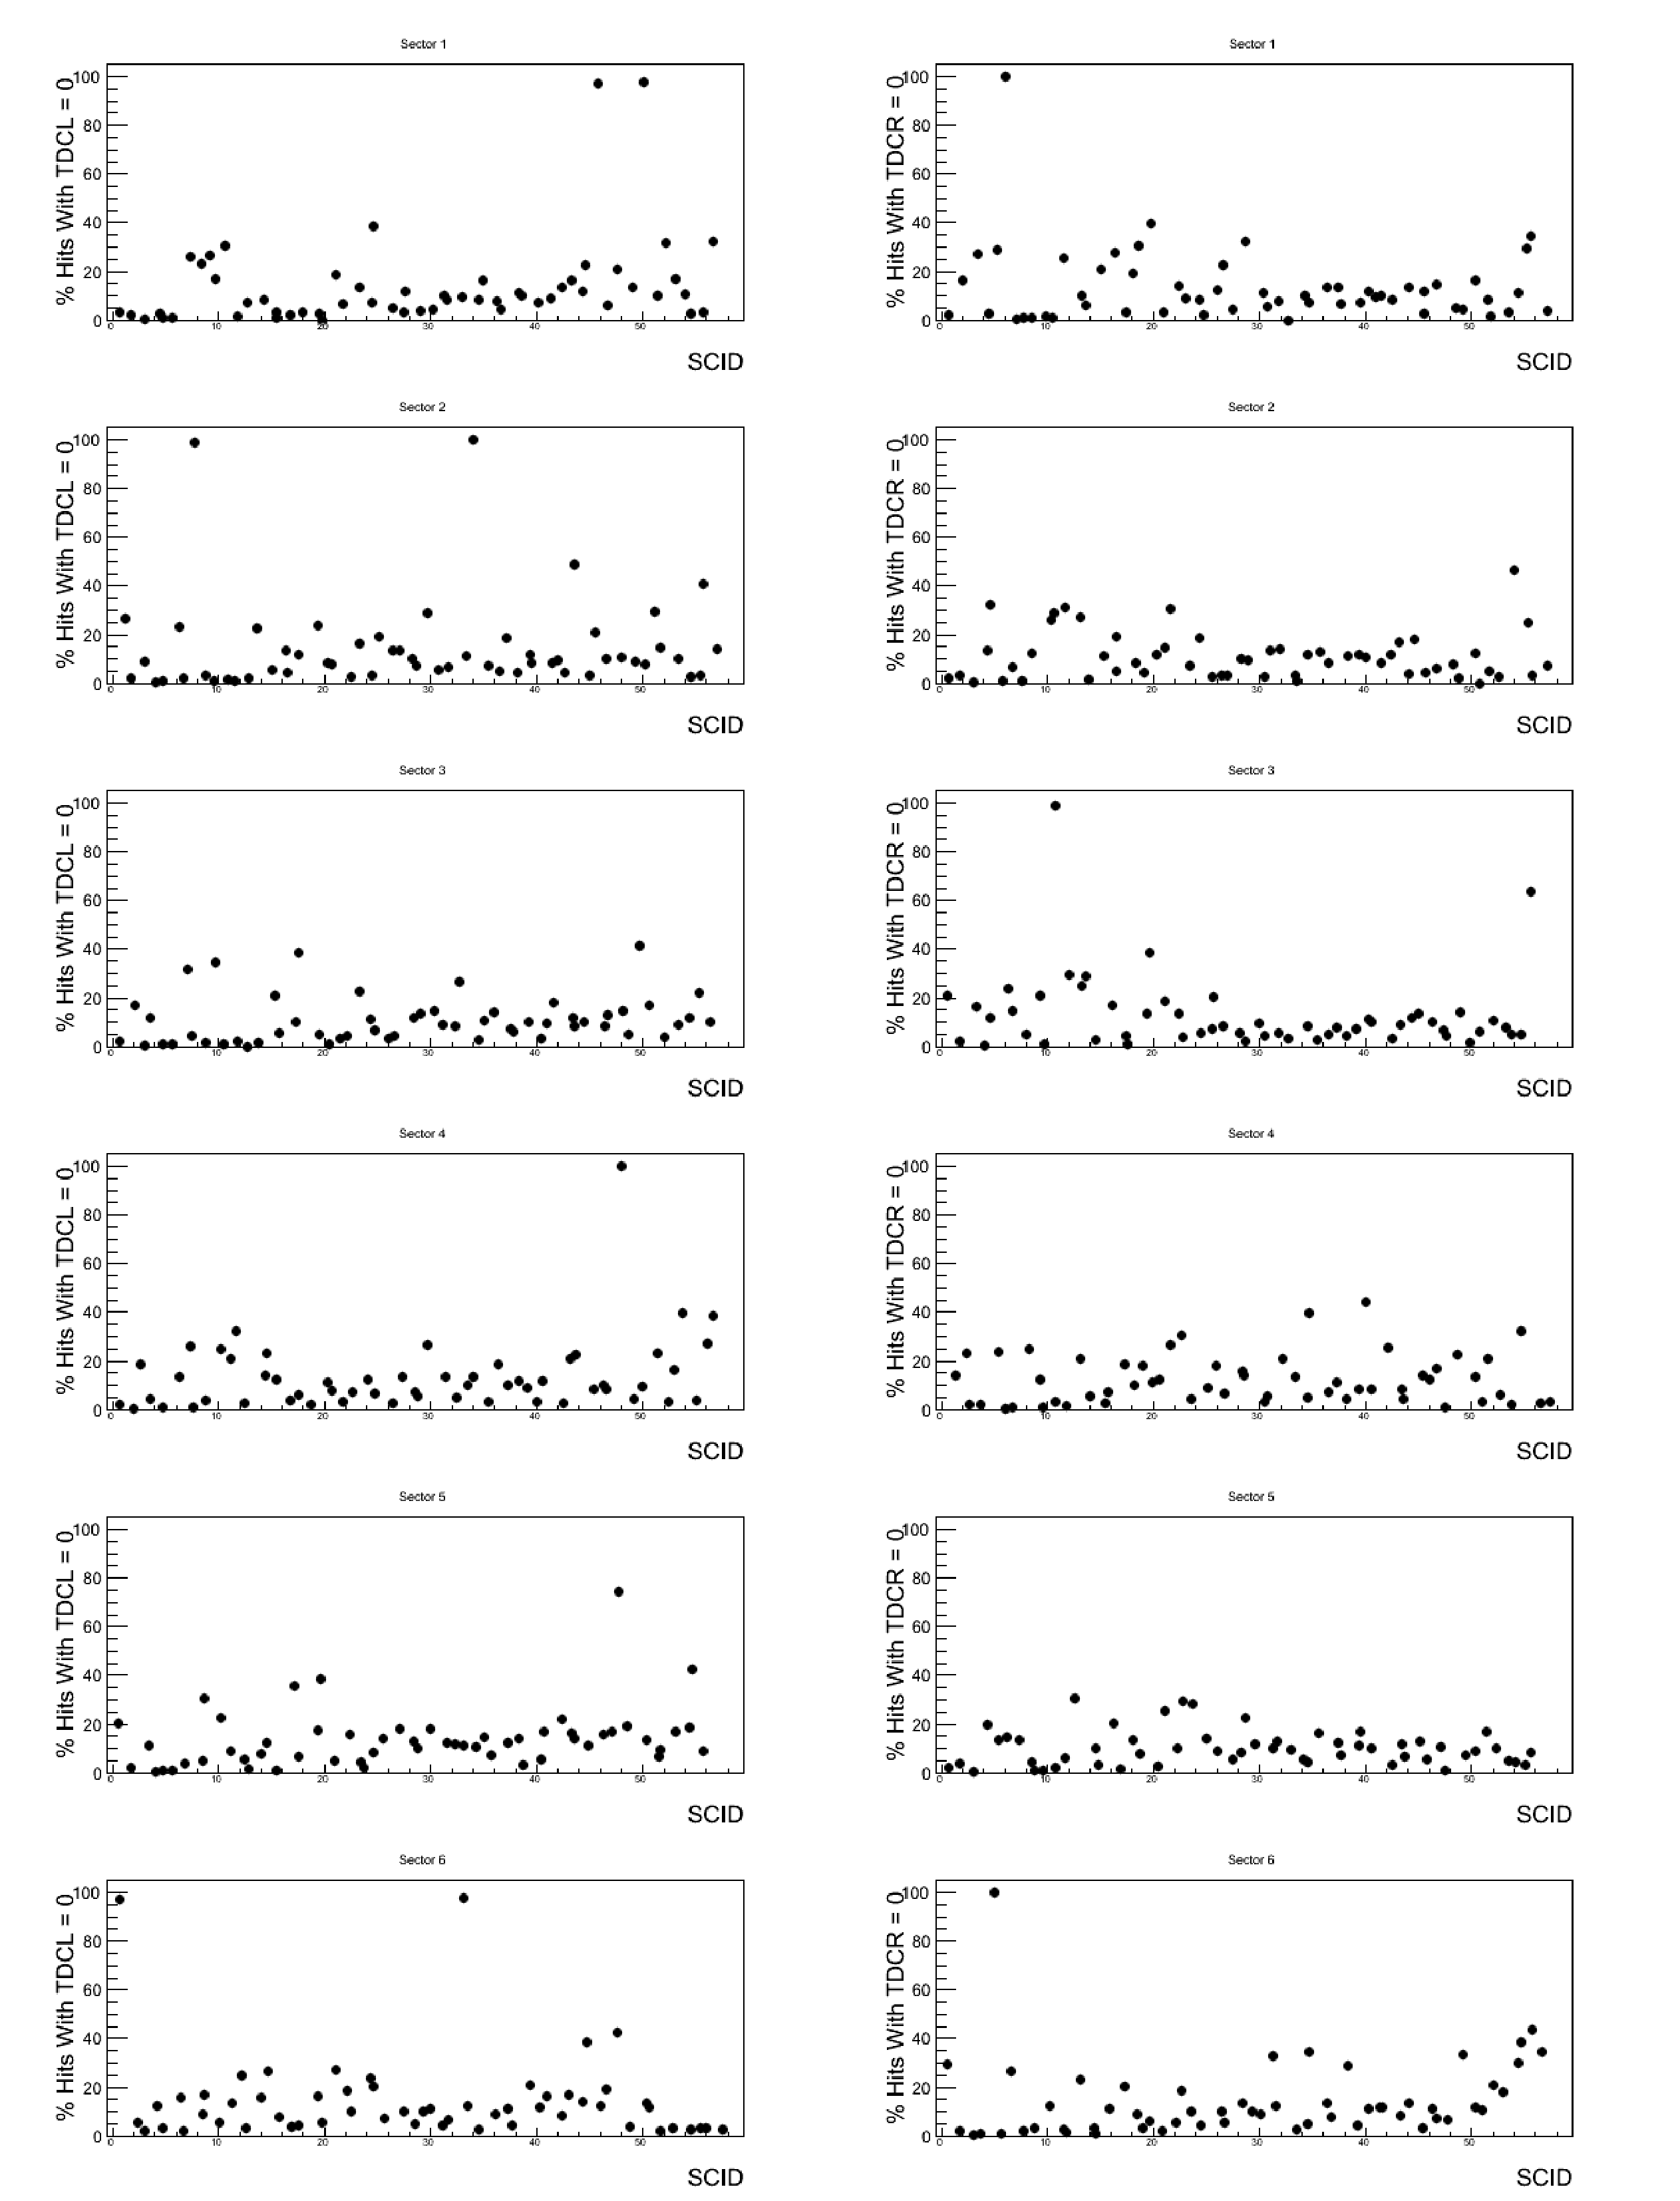
\includegraphics[width=0.8\textwidth]{figures/calib/tof/tofko/tdc.eps}
    \caption{Percentage of hits registering an TDC value of 0 for all scintillators. Left TDC (TDCL) are on the left and right TDC (TDCR) values are on the right}
    \label{plt:tdc0vSCID}
\end{figure}

\begin{figure}
    %\vspace{-16pt}
    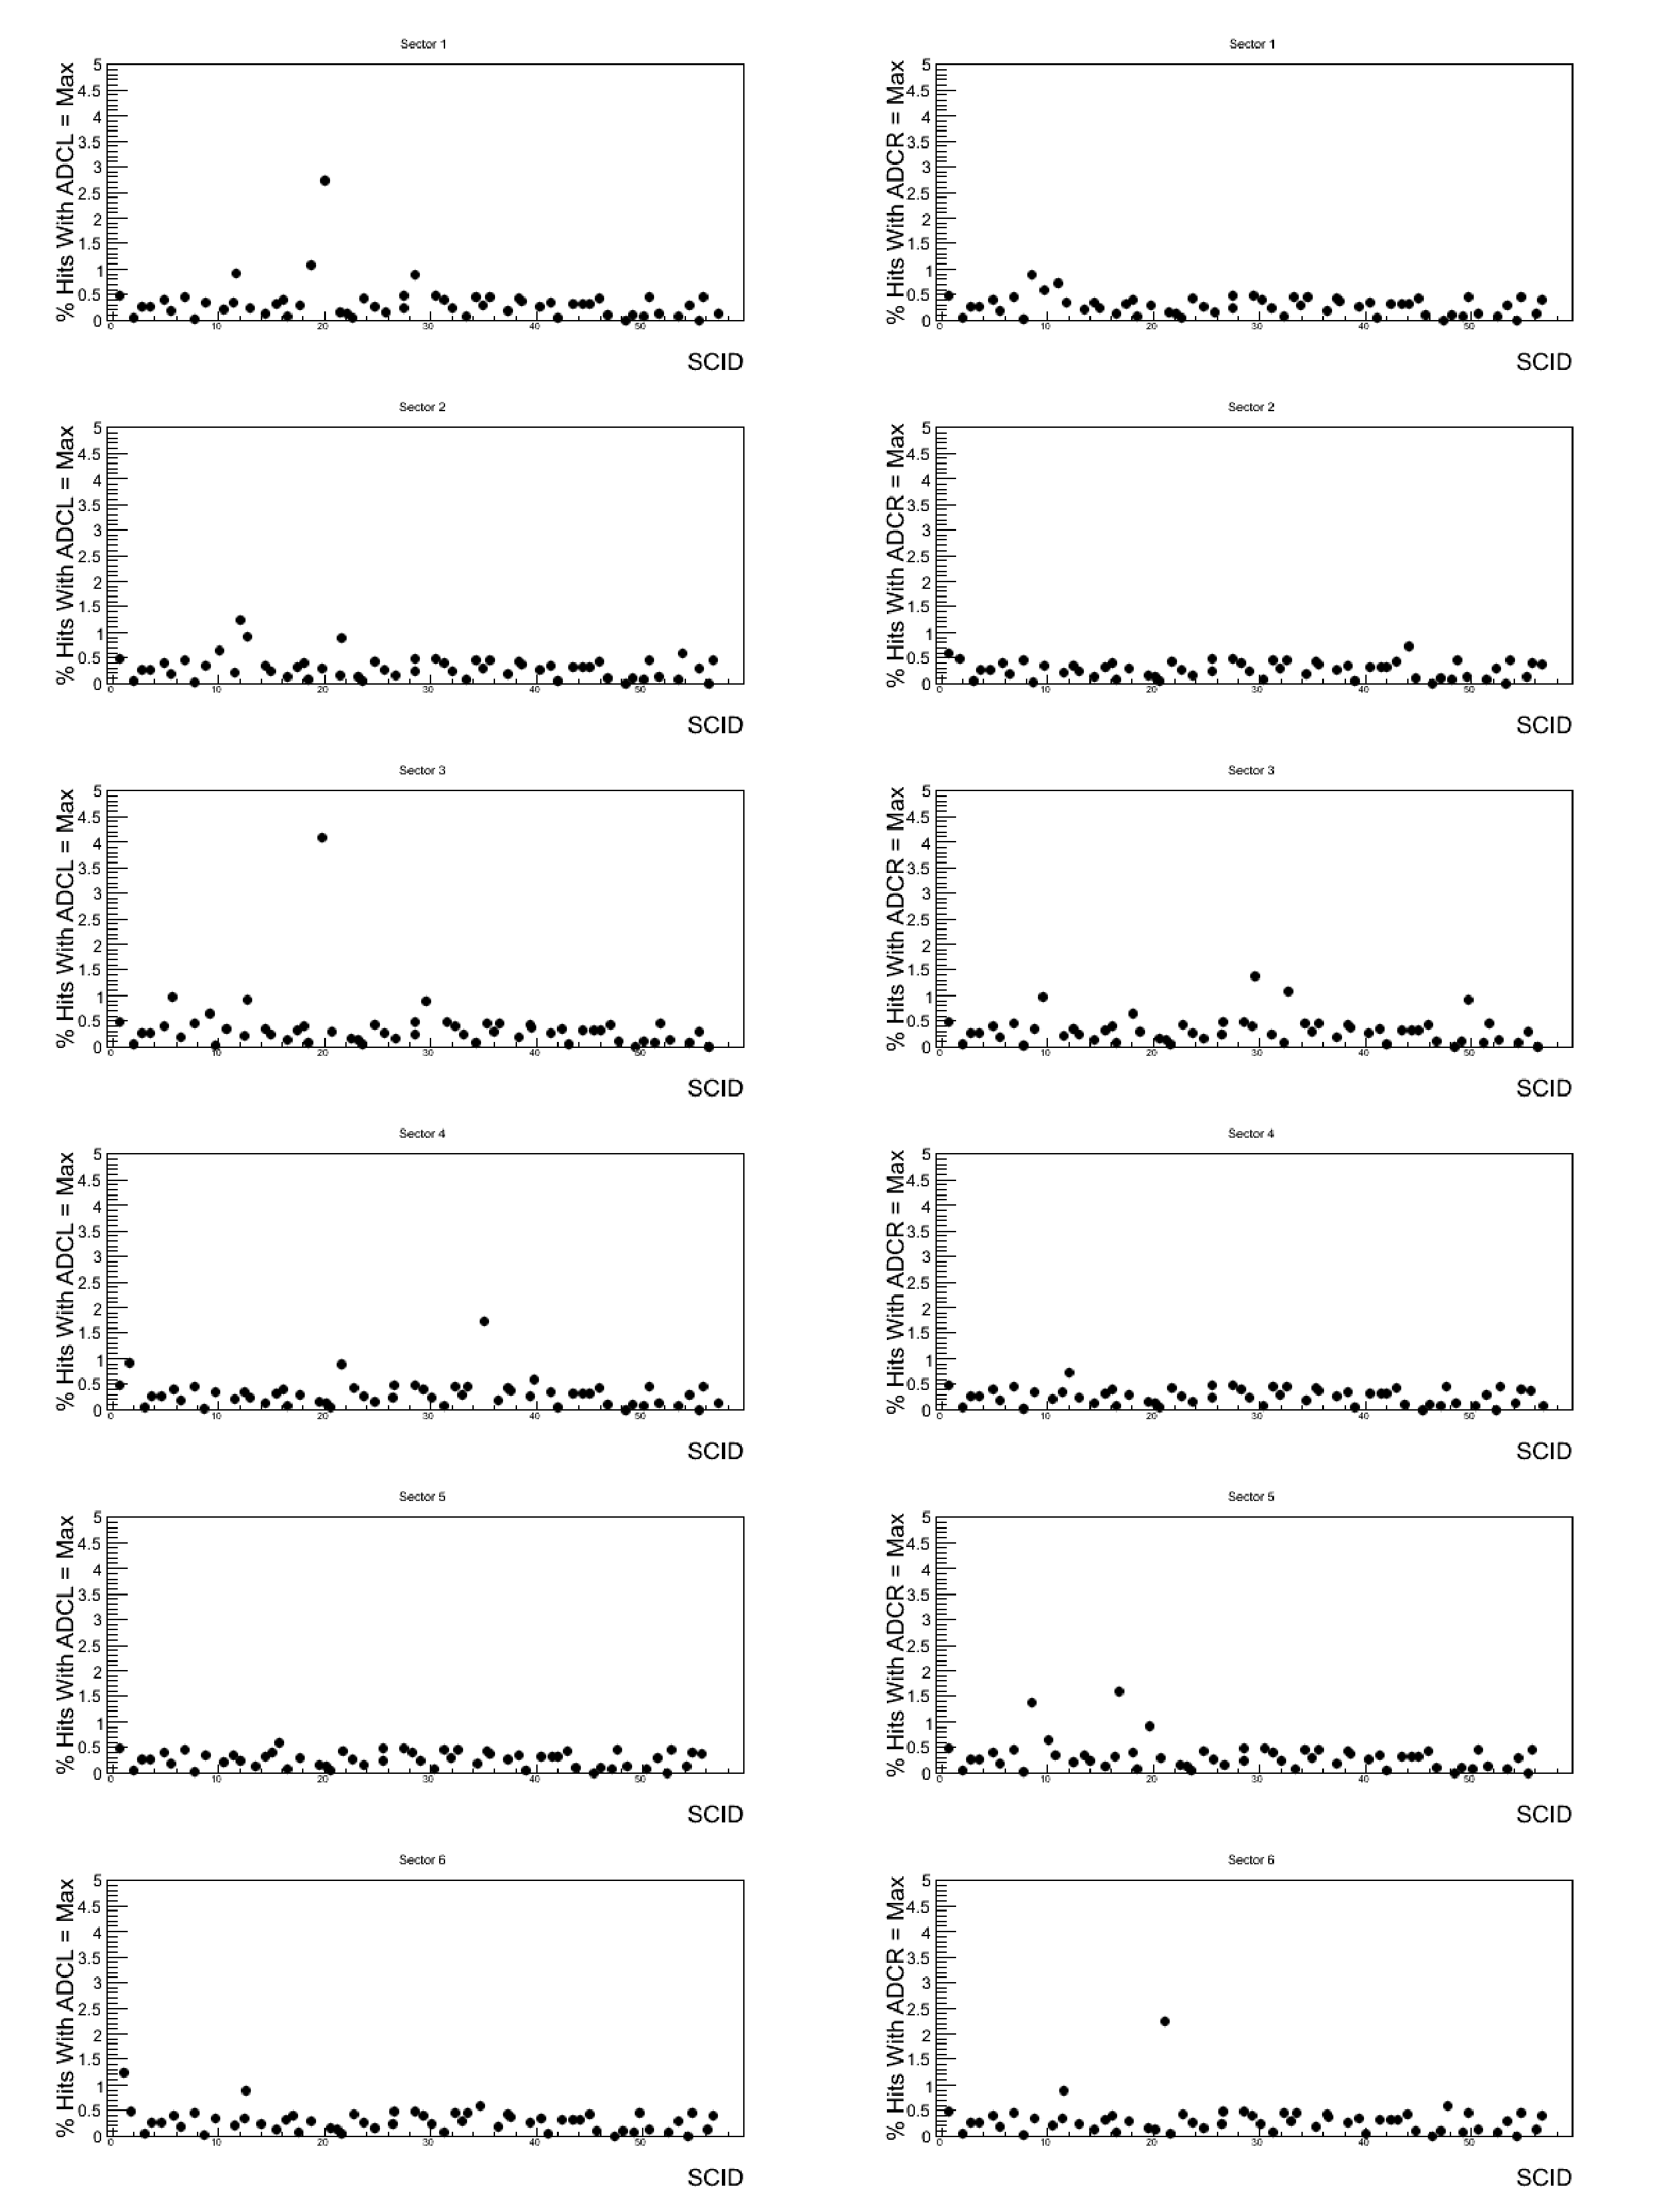
\includegraphics[width=0.8\textwidth]{figures/calib/tof/tofko/adcMax.eps}
    \caption{Percentage of hits registering a maximum ADC value for all scintillators. Left ADC (ADCL) are on the left and right ADC (ADCR) values are on the right}
    \label{plt:adcMvSCID}
\end{figure}

\begin{figure}
    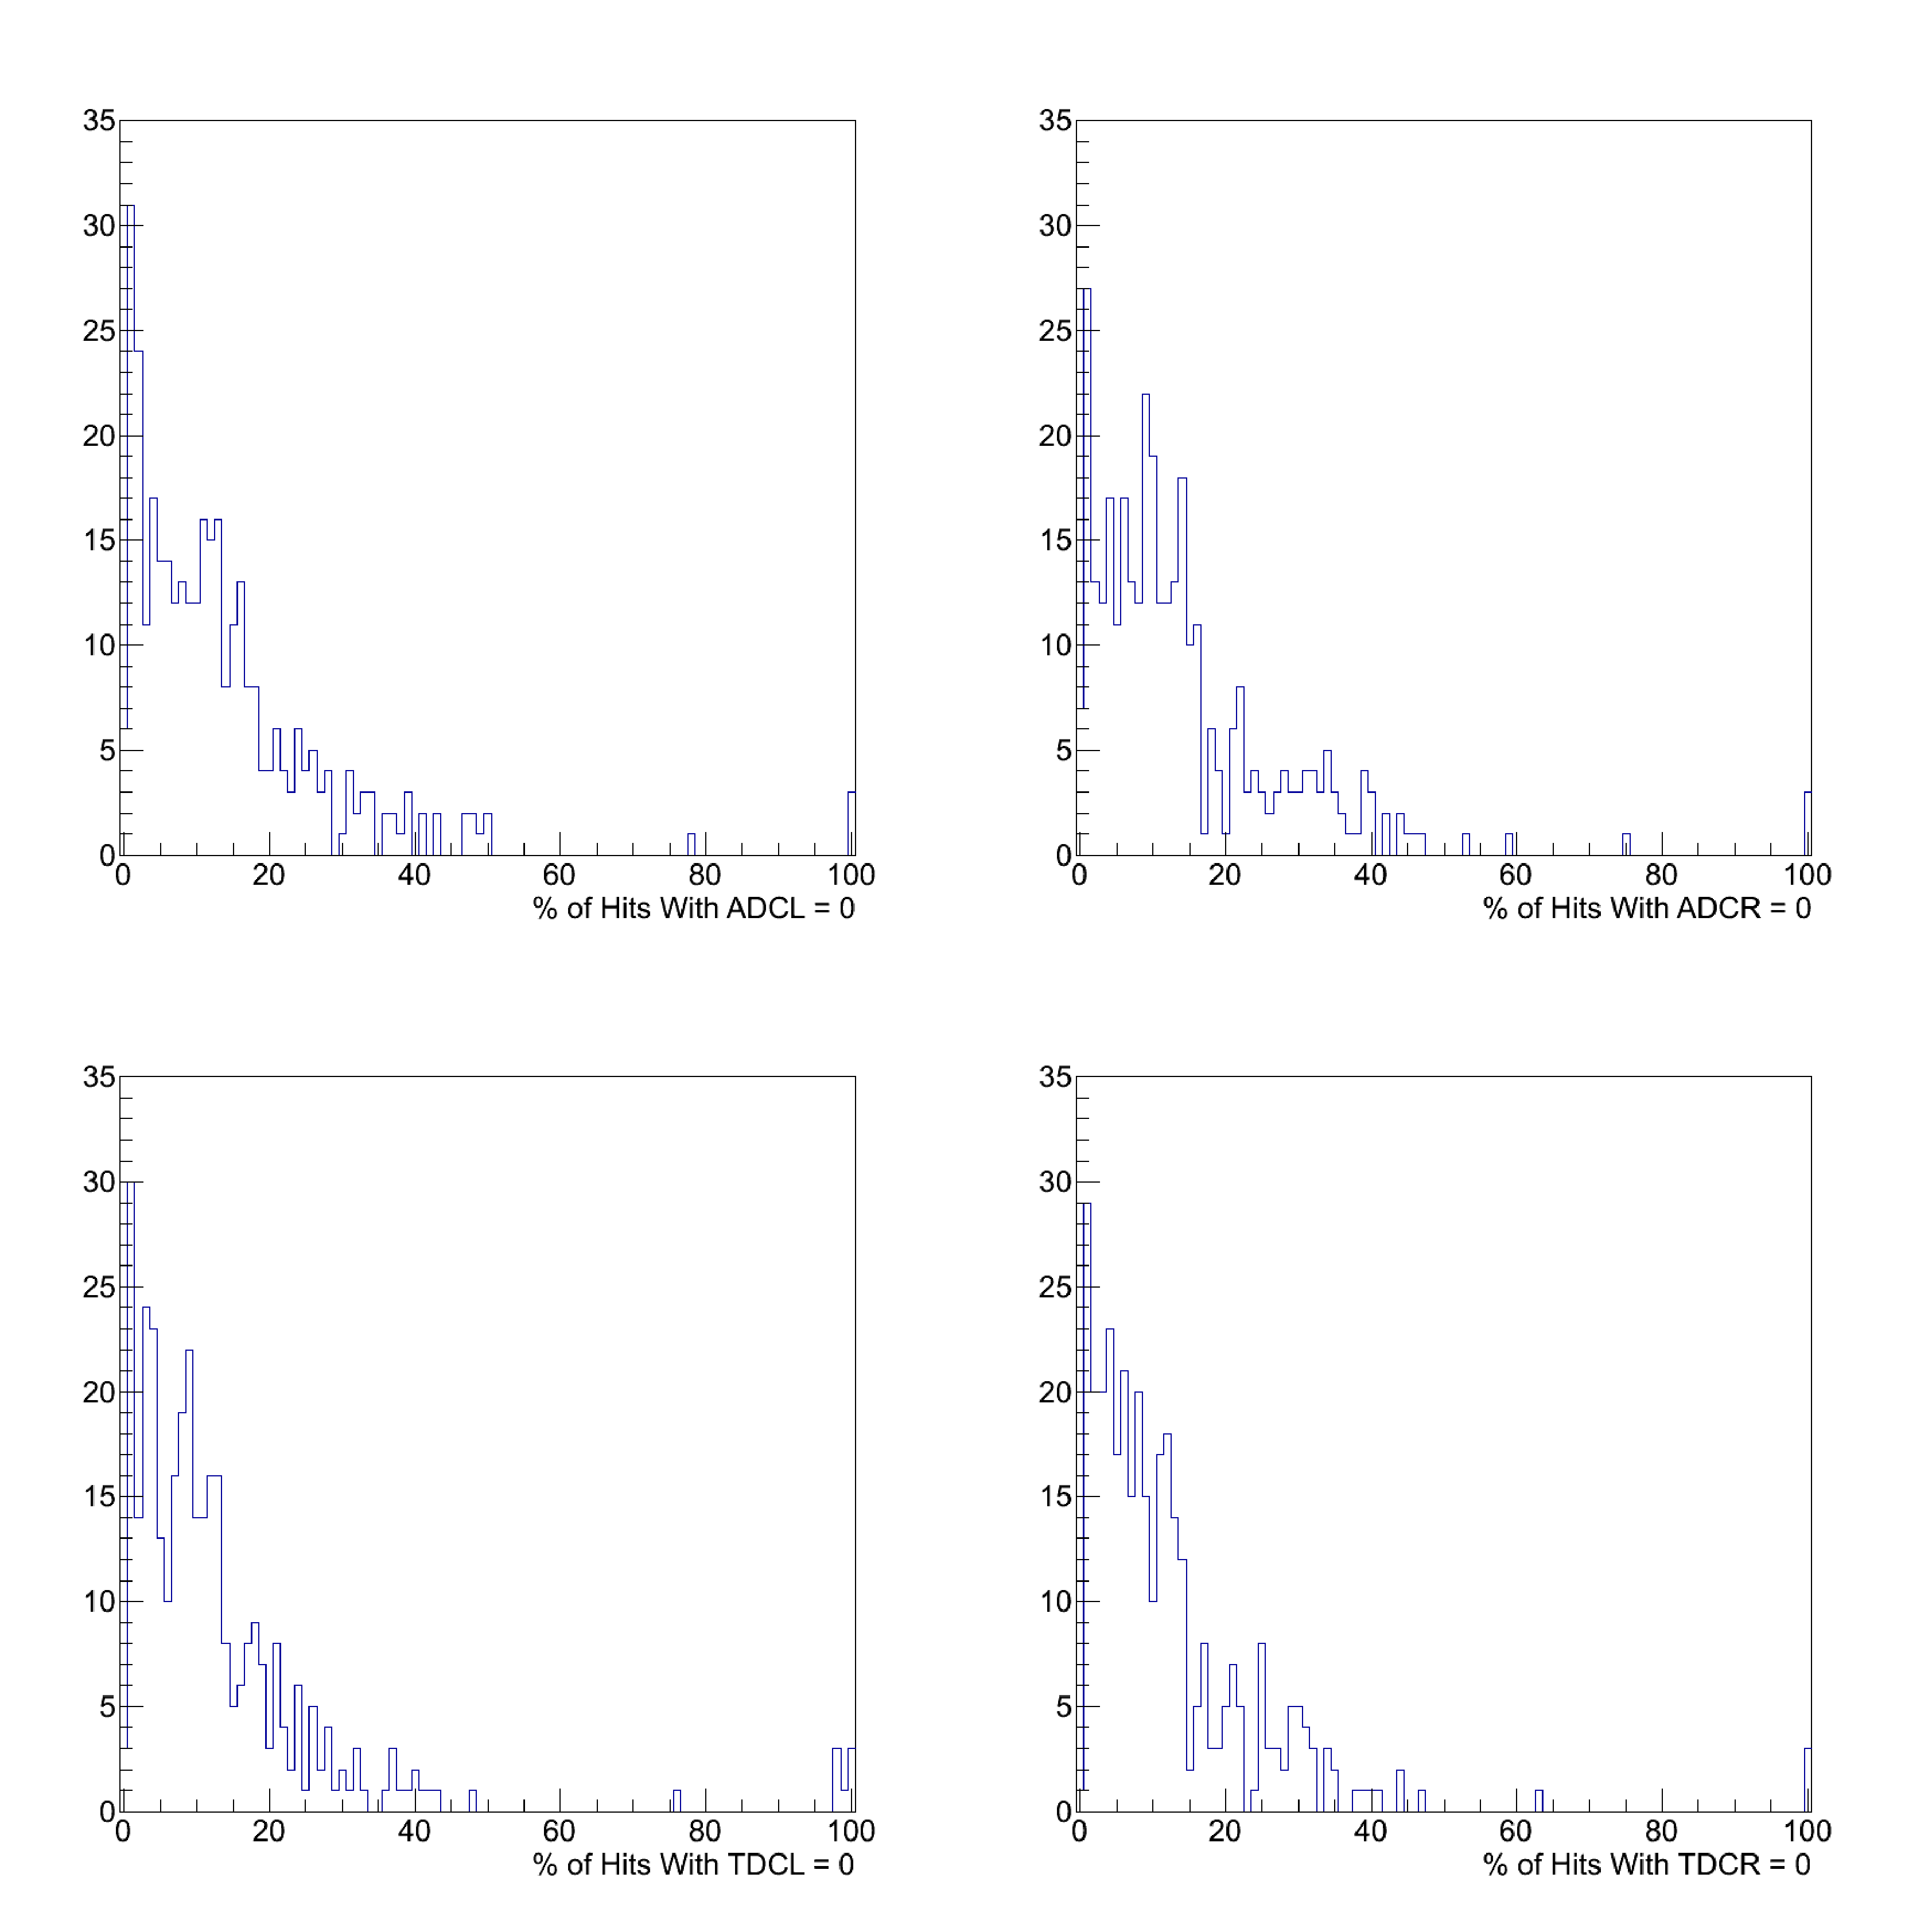
\includegraphics[width=0.8\textwidth]{figures/calib/tof/tofko/adctdc0perc.eps}
    \caption{Top: Y axis projections of \ref{plt:adc0vSCID}. Bottom: Y axis projections of \ref{plt:tdc0vSCID}}
    \label{plt:proj}
\end{figure}

\FloatBarrier

\subsection{\label{sec:calib.ec}Electrocalorimeter}

\subsubsection{\label{sec:calib.ec.eff}Electrocalorimeter Efficiency}

\FloatBarrier

\subsection{\label{sec:calib.pol}Beam Polarization}
The electron beam produced with a polarized laser incident on gallium arsenide allows for longitudinal polarization of the electrons~\cite{polarizedelectrons} and in turn, due to the bremsstrahlung process, circular polarization of the photon beam.  The accurate measurement of the polarization transferred from the photon beam to the produced hyperons ($C_x$ and $C_z$) requires knowledge of the beam polarization.  Such knowledge is ascertained by knowing the magnitude of incident electron-beam polarization, and the helicity orientation of the electron beam bunch responsible for the event (in the lab-frame). The Maximon-Olsen formula relating incident electron beam polarization, with the photon polarization is given by~\cite{MaximonOlsen},
\begin{equation}
P_\odot(E_\gamma) = \frac{x(4-x)}{4 - 4x + 3x^2}P_{elec}
\end{equation}
where $x = E_\gamma /E_{elec}$ is the ratio of photon energy, $E_\gamma$, to beam energy, $E_{elec}$. The g12 experiment ran with a constant electron energy of $E_{elec} = 5.715$ GeV.  (The actual electron beam energy was corrected on a run-by-run basis, see later section) The polarization of the electron beam was measured regularly using the a M{\o}ller polarimeter.  The polarimeter measures electron polarization by making use of the helicity dependent nature of M{\o}ller scattering~\cite{Mecking,Carman}. The M{\o}ller measurements, summarized in Fig.~\ref{moltable}, were performed regularly (every few days) during g12.  The run-integrated and flux -weighted value of the polarization of a particular range of photon energies can be easily obtained by using the maximum-Olsen formula.

\begin{figure}[h]
\begin{center}
 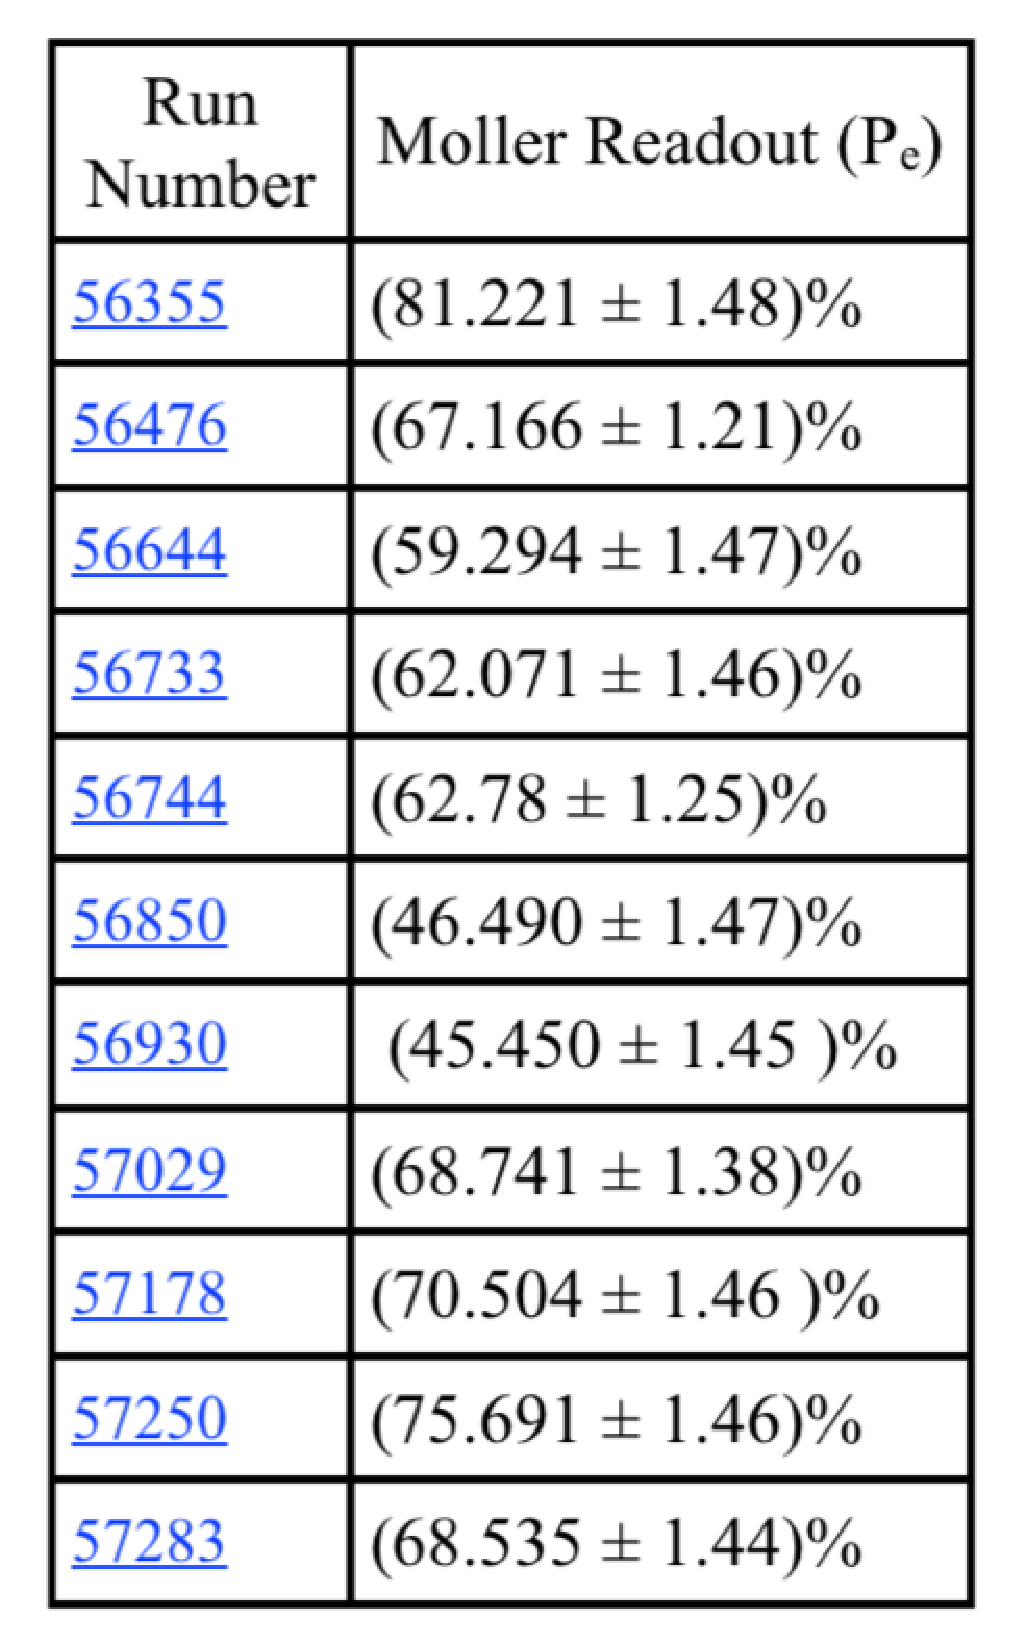
\includegraphics[width=0.9\textwidth]{figures/calib/pol/moltable.eps}
  \caption{The degree of longitudinal electron polarization ($P_e)$ for each M{\o}ller run. }
  \label{moltable}
  \end{center}
\end{figure}



An important experimental aspect of g12 is that the electron-beam helicity was flipped at a rate around 30 Hz. While the helicity information was recorded and stored in the HEVT bank for each event, the convention for bit encoding has been known to change from real-time to delayed-time recording. Further considerations, such as the half-wave plate orientation also had to be accounted for.

The only sure way to pin down the absolute beam helicity orientation for our data was to analyze a well known helicity-dependent reaction. Well-established results in Ref.~\cite{Io} in the beam-helicity asymmetry, $I^\odot(\phi^{hel}_\pi)$, for the reaction, $\gamma p \to p \pi^+ \pi^-$, were reproduced.  The mentioned reaction was shown to have a specific helicity-frame defined $\phi^{hel}_{\pi^+}$-dependent structure.  If the helicity convention was reversed then we would observe $I^\odot(\phi^{hel}_{\pi^+}) \to -I^\odot(\phi^{hel}_{\pi^+})$.

The sub-analysis we performed required exclusive $p \pi^+ \pi^-$ events in the final state. To ensure exclusivity we required zero missing energy and momentum within detector resolution. The helicity frame (shown in Fig.~\ref{ioplane}) was defined to be the rest frame of the hypothetical parent meson of the two pion system, with  $\hat{z}$ aligned along its center-of-mass defined momentum. $\phi^{hel}_{\pi^+}$ is the angle between the proton-production plane, and the plane containing both pions. The beam helicity asymmetry is given by,
\begin{equation}
I_\odot = \frac{N^+ - N^-}{N^+ + N^-},
\end{equation}
where $N^\pm$ indicates the number of events with positive (negative) photon helicity.  Figs.~\ref{myIo}-\ref{Io} show the $I_{\odot}(\phi^{hel}_{\pi^+})$ for g12 and in the analysis of \cite{Io}.
The lab-frame electron helicity readout was taken from the HEVT bank (HEVT$\to$hevt[0].TGRPRS). The results of our $I_{\odot}(\phi^{hel}_{\pi^+})$ analysis and the previously published results showed a positive (negative) HEVT readout indicates positive (negative) photon helicity. The reproduction of beam-helicity asymmetry for double charged pion production also served as a way to test the accuracy of the calculated photon polarization magnitude: both results' wave amplitudes were in good agreement.

\begin{figure}[h]
\begin{center}
 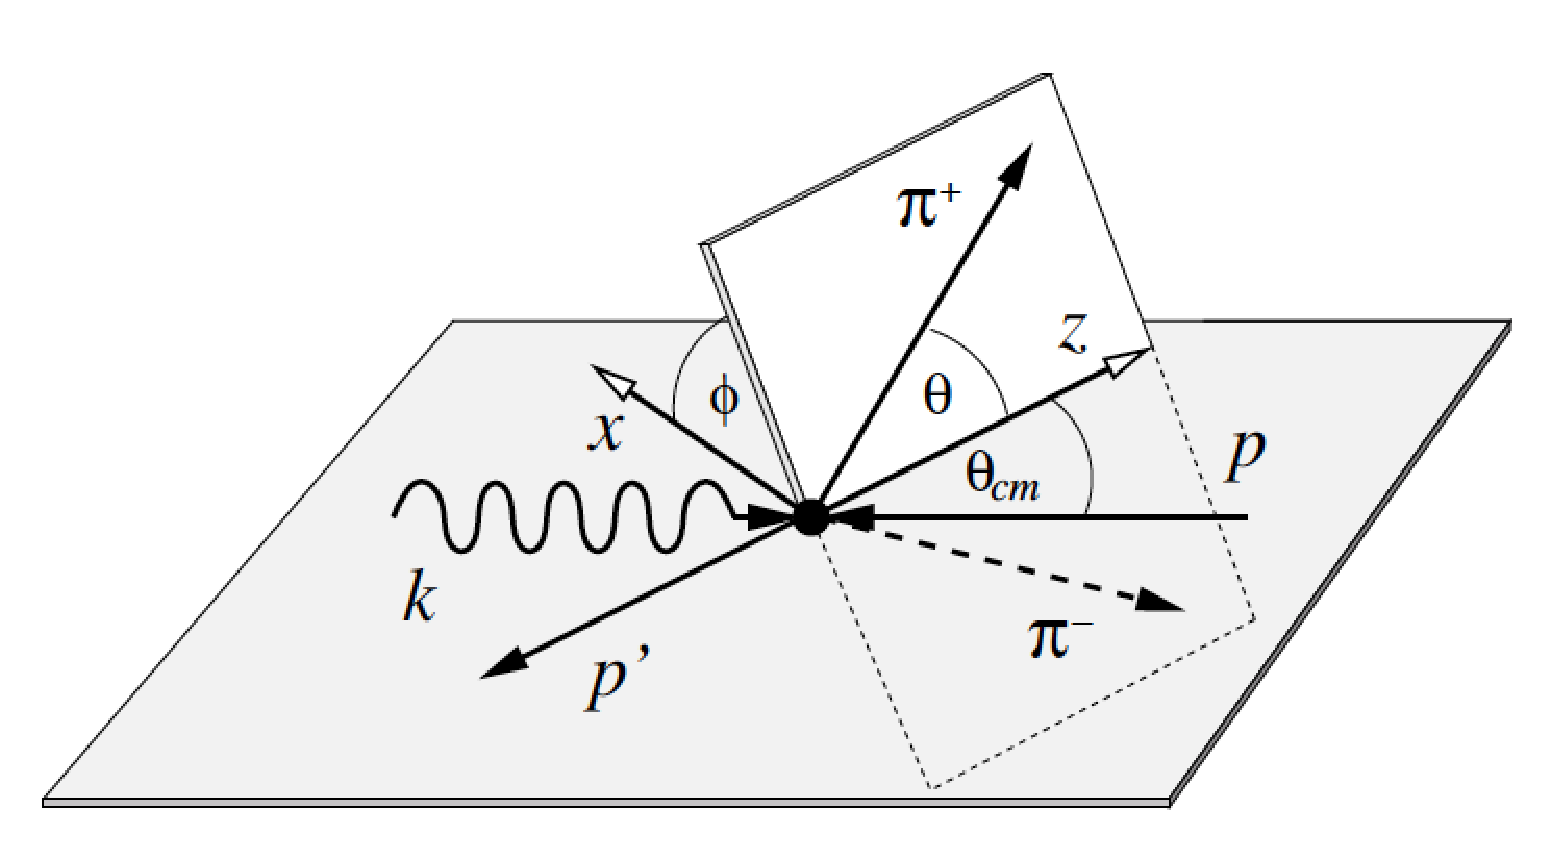
\includegraphics[width=0.9\textwidth]{figures/calib/pol/ioplane.eps}
  \caption{An illustration of the angle definitions used in the $\gamma p \to \pi^+ \pi^- p$ sub-analysis. $\theta_{cm}$ is defined in the center-of-mass frame. $\theta$ and $\phi$ are defined in the rest frame of the $\pi^+$ $\pi^-$ system as the polar and azimuthal angles. The $z$ direction is along the total momentum of the $\pi^+ \pi^-$ system.}
  \label{ioplane}
  \end{center}
\end{figure}


\begin{figure}[h]
\begin{center}
 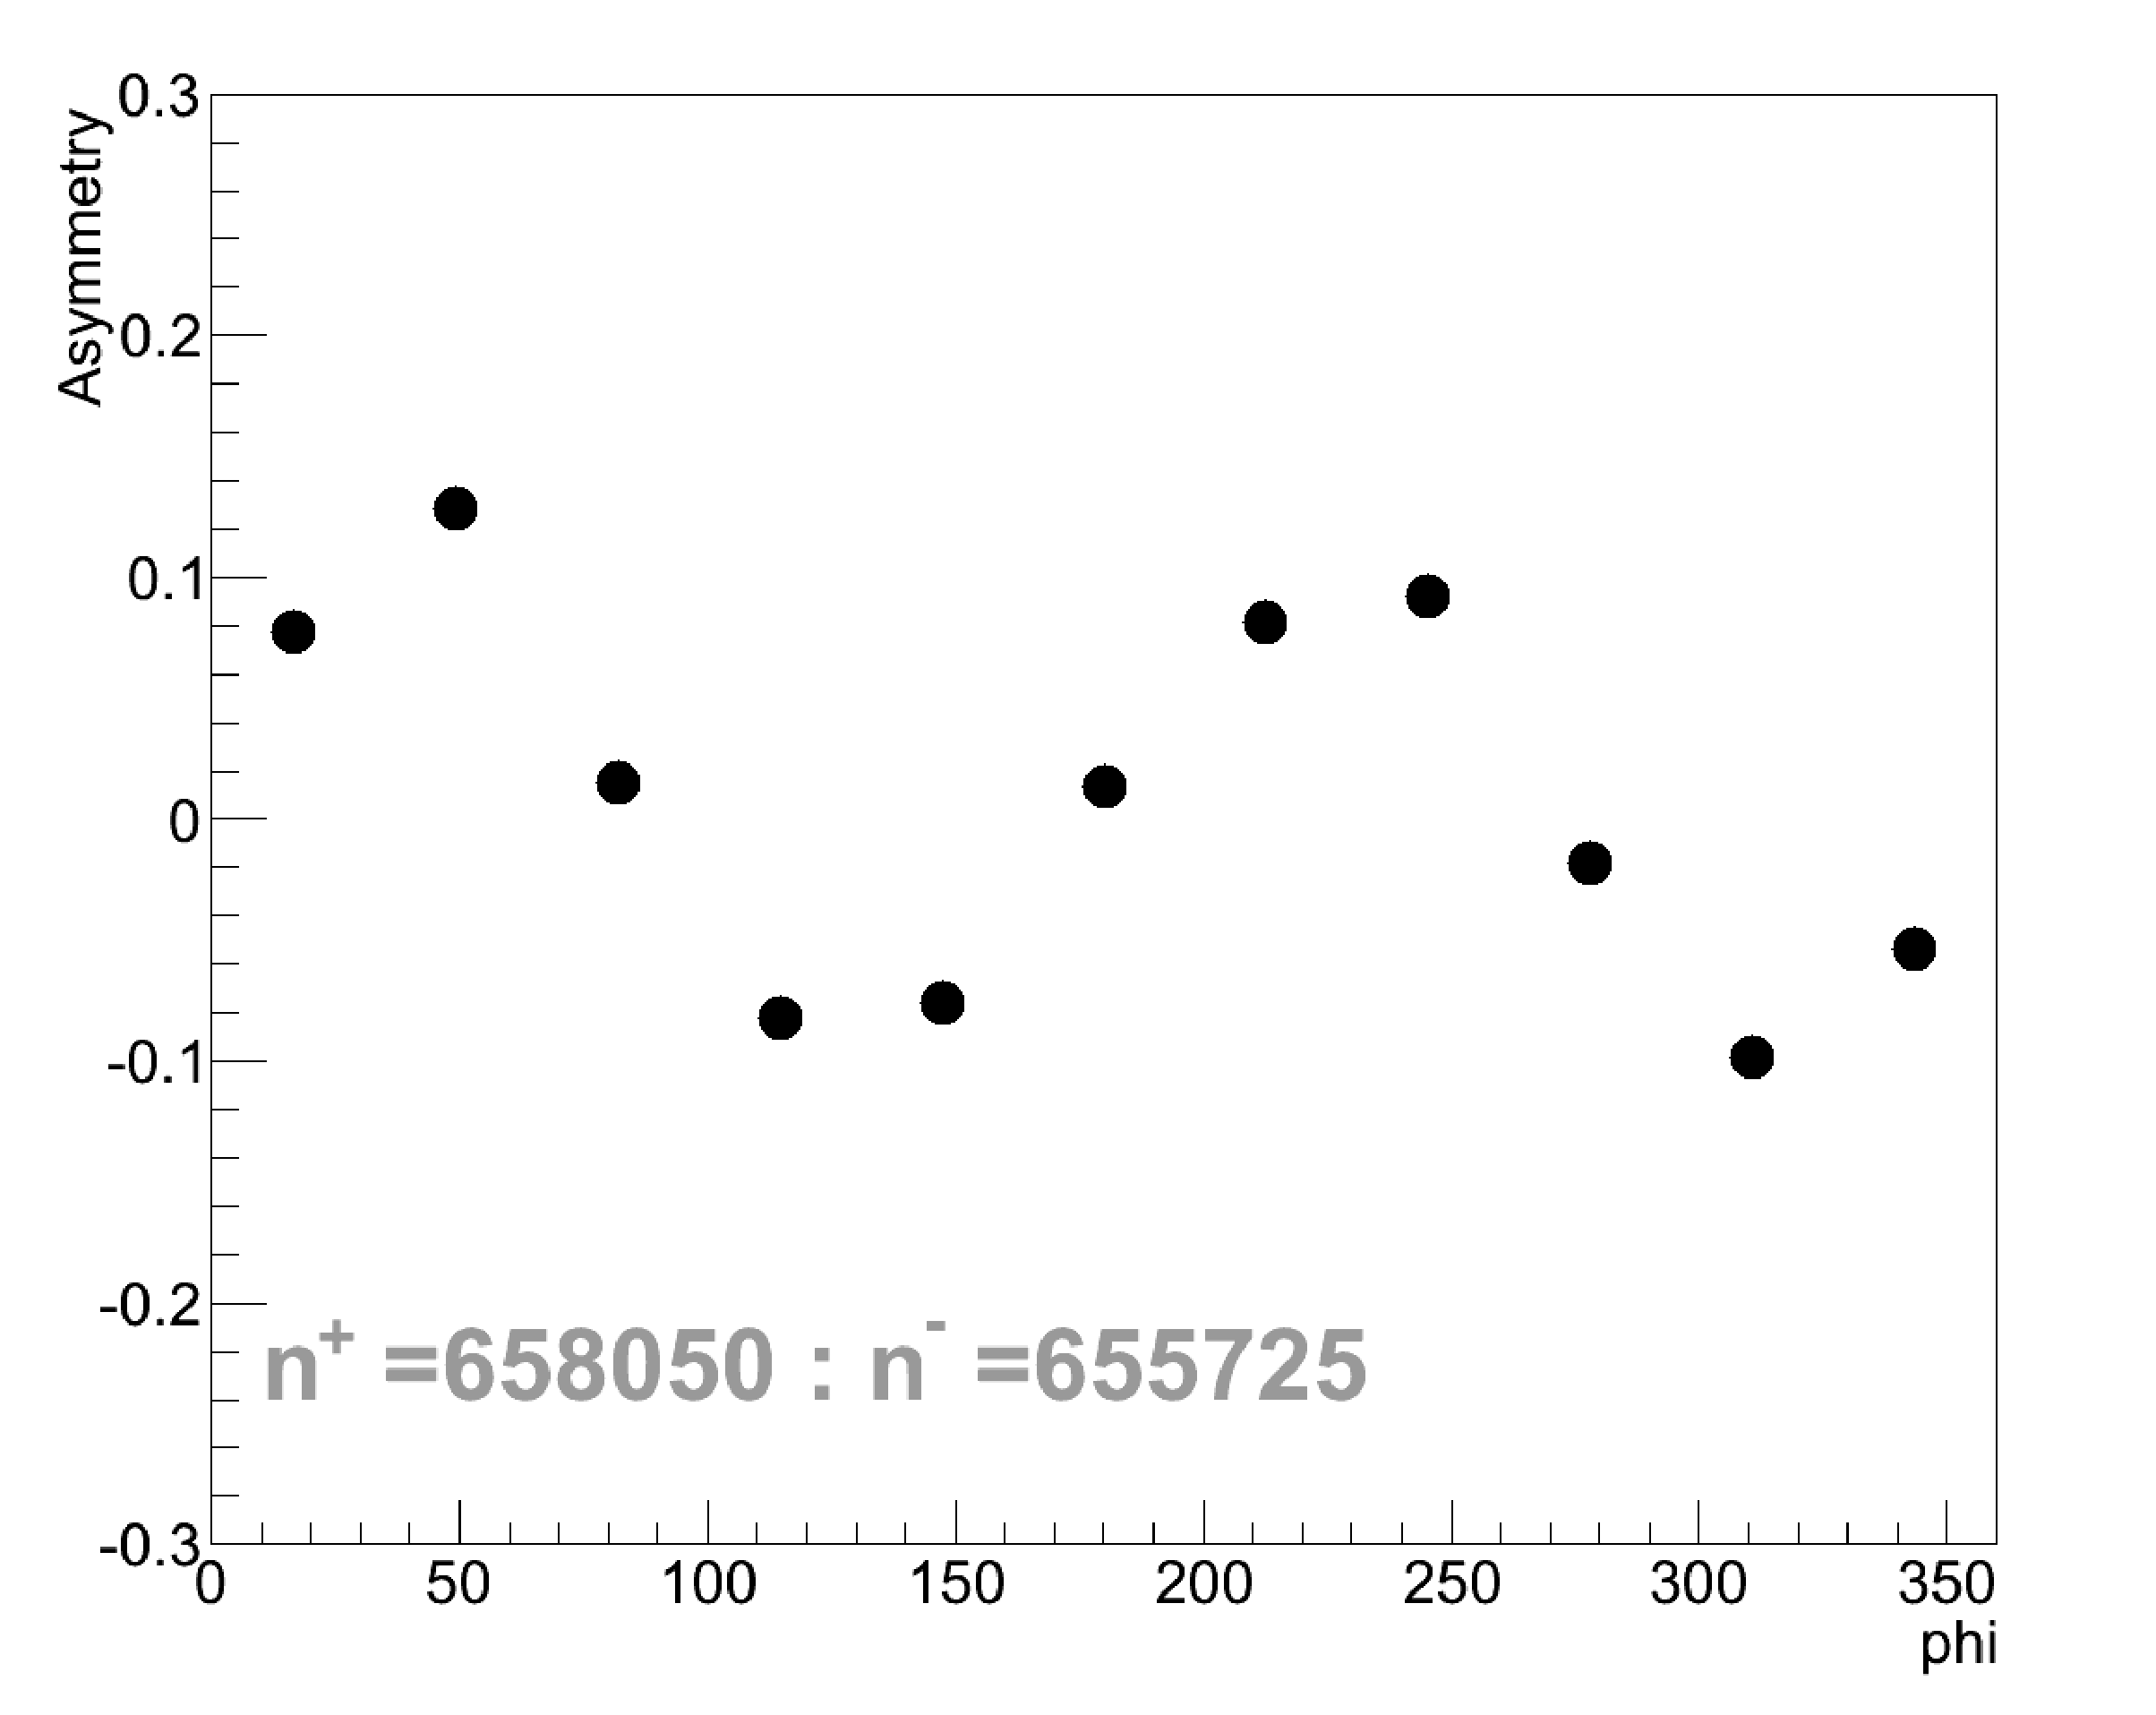
\includegraphics[width=0.9\textwidth]{figures/calib/pol/myIo.eps}
  \caption{$I_{\odot}(\phi^{hel}_{\pi^+})$ for g12 data within the energy range of $W = 1.9-2.3$ GeV.}
  \label{myIo}
  \end{center}
\end{figure}


\begin{figure}[h]
\begin{center}
 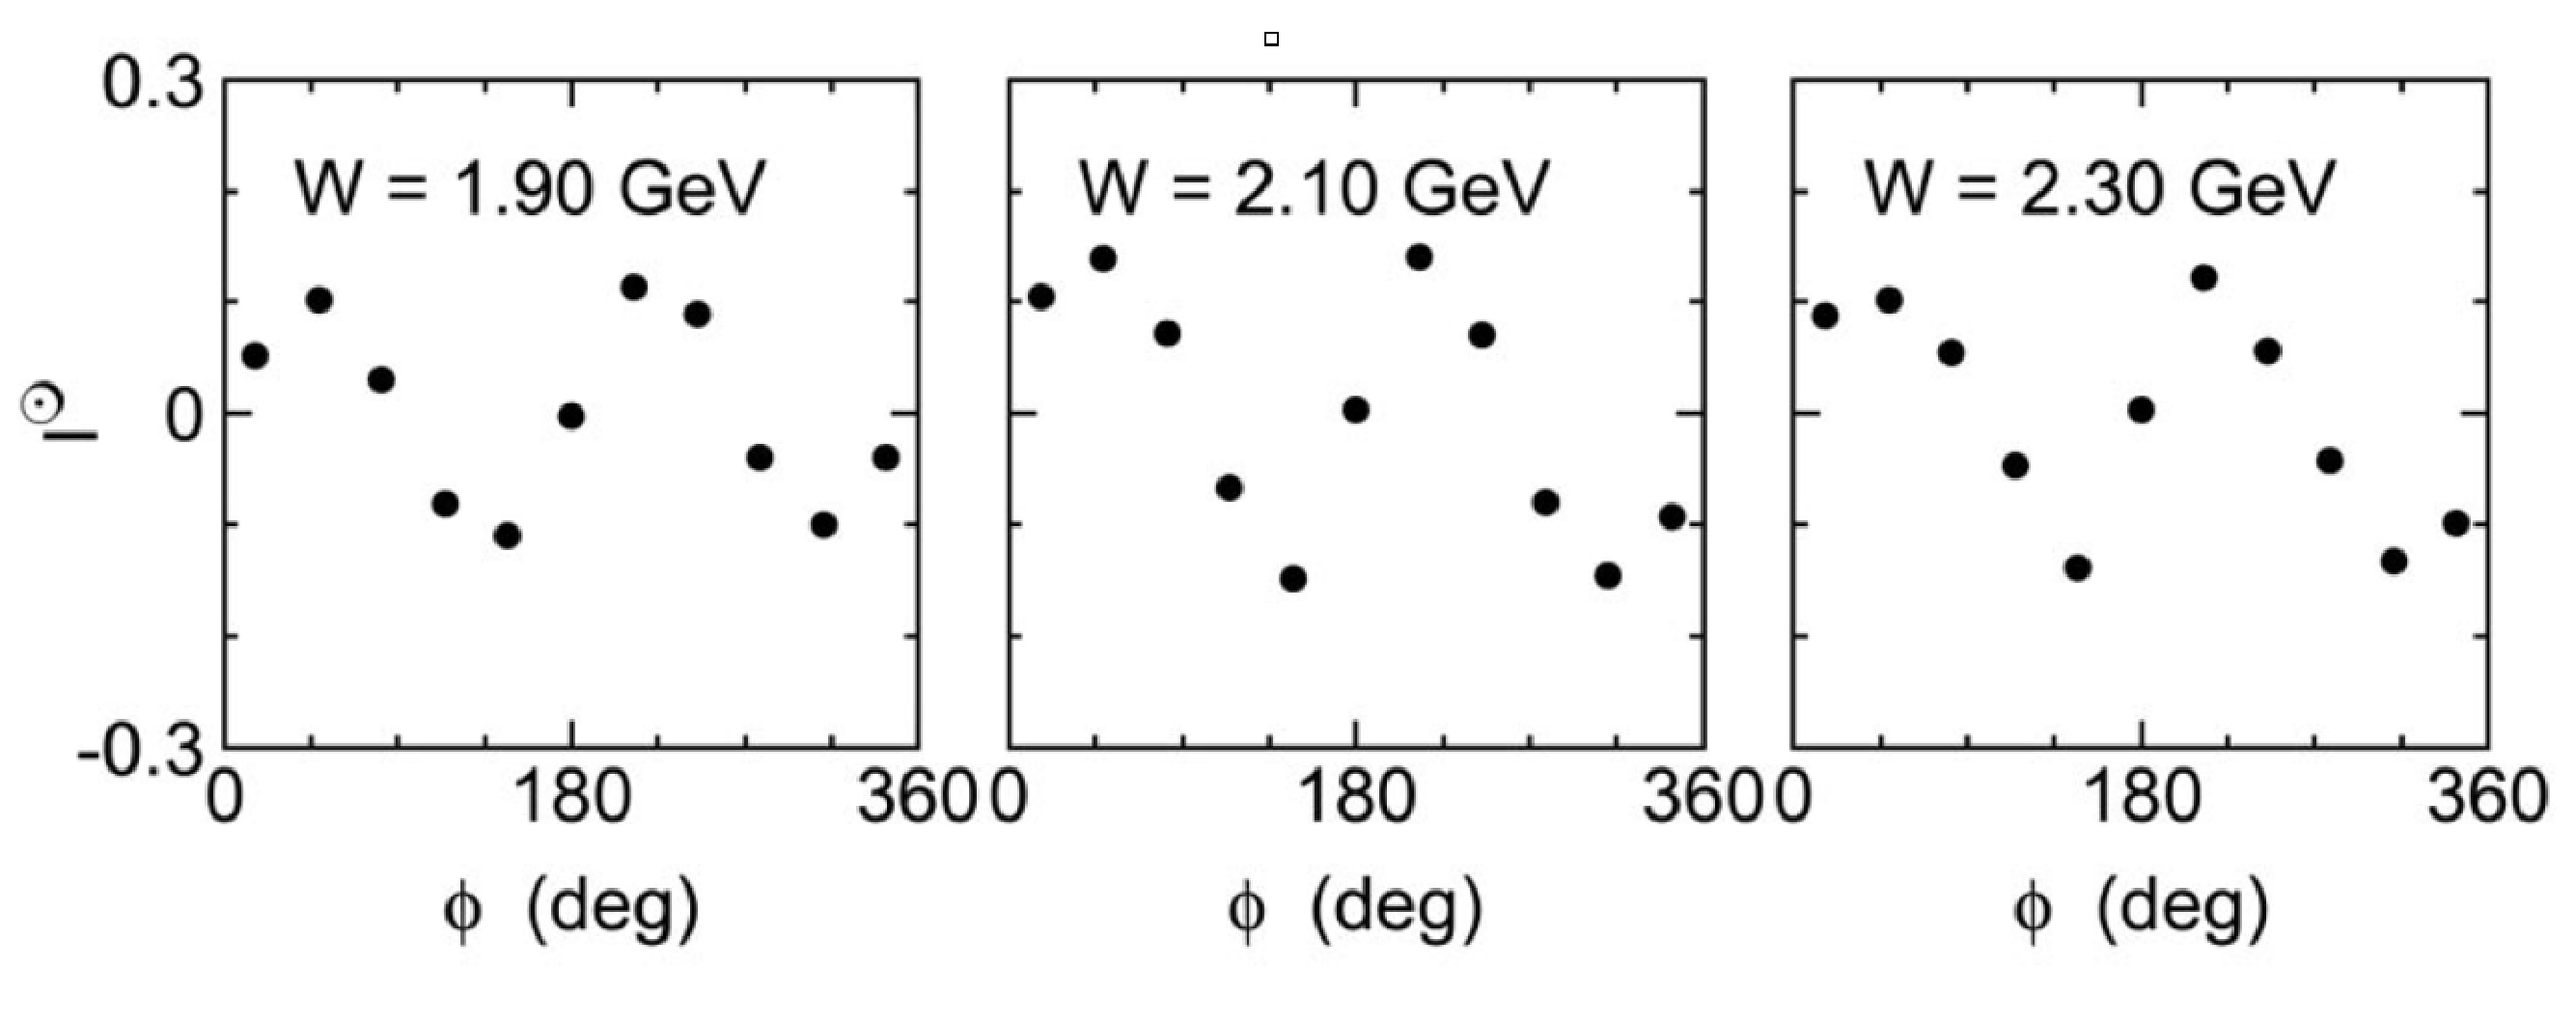
\includegraphics[width=0.9\textwidth]{figures/calib/pol/Io.eps}
  \caption{$I_{\odot}(\phi^{hel}_{\pi^+})$ as measured in the previous analysis.}{ $I_{\odot}(\phi^{hel}_{\pi^+})$ as measured in the analysis~\cite{Io}. The results of are shown in bins of $W$ from $1.9$ to 2.3 GeV.}
  \label{Io}
  \end{center}
\end{figure}




To conclude, the g12 beam polarization was measured with standard methods, and the validity of the photon helicity definition in the HEVT bank was double checked against existing experimental results and confirmed to be correct. All g12 measurements that utilizes the beam polarization refer to what has been summarized here.



